\RequirePackage[l2tabu,orthodox]{nag}

% TODO: decide if one-sided/two-sided
%\documentclass[headsepline,footsepline,footinclude=false,fontsize=11pt,paper=a4,listof=totoc,bibliography=totoc,BCOR=12mm,DIV=12]{scrbook} % two-sided
\documentclass[headsepline,footsepline,footinclude=false,oneside,fontsize=11pt,paper=a4,listof=totoc,bibliography=totoc]{scrbook} % one-sided

\PassOptionsToPackage{table,svgnames,dvipsnames}{xcolor}

\usepackage[utf8]{inputenc}
\usepackage[T1]{fontenc}
\usepackage[sc]{mathpazo}
\usepackage[american]{babel}
\usepackage[autostyle]{csquotes}
\usepackage[%
  backend=biber,
  url=false,
  style=alphabetic,
  maxnames=4,
  minnames=3,
  maxbibnames=99,
  firstinits,
  uniquename=init]{biblatex} % TODO: adapt bibliography style
\usepackage{graphicx}
\usepackage{scrhack} % necessary for listings package
\usepackage{listings}
\usepackage{lstautogobble}
\usepackage{tikz}
\usepackage{pgfplots}
\usepackage{pgfplotstable}
\usepackage{booktabs}
\usepackage[final]{microtype}
\usepackage{caption}
\usepackage[hidelinks]{hyperref} % hidelinks removes colored boxes around references and links
\addto\extrasenglish{%
  \def\chapterautorefname{Chapter}%
  \def\sectionautorefname{Section}%
}

%\usepackage{cleveref}
\usepackage[toc,nonumberlist,acronym]{glossaries} % TODO: remove if glossary not needed

\usepackage{color}
\usepackage[section]{placeins}
\usepackage{float}
\usepackage{xcolor}

\usepackage{pgf-umlsd}
\usetikzlibrary{arrows,shadows,snakes,backgrounds}

\usepackage{verbatim}
\usepackage{pbox}
\usepackage{framed}
\usepackage{adjustbox}
\usepackage{graphicx}
\usepackage{amsfonts}
\usepackage{multirow}
\usepackage{amsmath,amssymb,amsthm,enumitem}
\usepackage{rotating}
\usepackage{framed}
\usepackage{multicol}
\bibliography{bibliography/literature}

\setkomafont{disposition}{\normalfont\bfseries} % use serif font for headings
\linespread{1.05} % adjust line spread for mathpazo font

% Settings for glossaries TODO: remove the following block if glossary not needed
\renewcommand{\glsnamefont}[1]{\normalfont\bfseries #1} % use serif font for glossary entry titles
\makeglossaries{}

% Settings for pgfplots
\pgfplotsset{compat=1.9} % TODO: adjust to your installed version
\pgfplotsset{
  % For available color names, see http://www.latextemplates.com/svgnames-colors
  cycle list={CornflowerBlue\\Dandelion\\ForestGreen\\BrickRed\\},
}

\definecolor{pblue}{rgb}{0.13,0.13,1}
\definecolor{pgreen}{rgb}{0,0.5,0}
\definecolor{pred}{rgb}{0.9,0,0}
\definecolor{pgrey}{rgb}{0.46,0.45,0.48}

\colorlet{punct}{red!60!black}
\definecolor{background}{HTML}{EEEEEE}
\definecolor{delim}{RGB}{20,105,176}
\colorlet{numb}{magenta!60!black}


% \lstdefinestyle{customJava}{
% belowcaptionskip=1\baselineskip,
% breaklines=true,
% frame=L,
% xleftmargin=\parindent,
% language=Java,
% showstringspaces=false,
% showspaces=false,
% backgroundcolor=\color{background},
% breakatwhitespace=true,
% basicstyle=\footnotesize\ttfamily,
% commentstyle=\color{pgreen},
% keywordstyle=\color{pblue},
% stringstyle=\color{pred},
% moredelim=[il][\textcolor{pgrey}]{\$},
% moredelim=[is][\textcolor{pgrey}]{\%\%}{\%\%}
% }

\lstdefinestyle{customJava}{
basicstyle=\normalfont\ttfamily,
belowcaptionskip=1\baselineskip,
numbers=left,
numberstyle=\scriptsize,
stepnumber=1,
numbersep=8pt,
breaklines=true,
frame=lines,
xleftmargin=\parindent,
language=Java,
showstringspaces=false,
showspaces=false,
backgroundcolor=\color{background},
breakatwhitespace=true,
commentstyle=\color{pgreen},
keywordstyle=\color{pblue},
stringstyle=\color{pred},
moredelim=[il][\textcolor{pgrey}]{\$},
moredelim=[is][\textcolor{pgrey}]{\%\%}{\%\%}
}

\lstdefinelanguage{json}{
basicstyle=\normalfont\ttfamily,
numbers=left,
numberstyle=\scriptsize,
stepnumber=1,
numbersep=8pt,
showstringspaces=false,
breaklines=true,
frame=lines,
backgroundcolor=\color{background},
literate=
*{0}{{{\color{numb}0}}}{1}
{1}{{{\color{numb}1}}}{1}
{2}{{{\color{numb}2}}}{1}
{3}{{{\color{numb}3}}}{1}
{4}{{{\color{numb}4}}}{1}
{5}{{{\color{numb}5}}}{1}
{6}{{{\color{numb}6}}}{1}
{7}{{{\color{numb}7}}}{1}
{8}{{{\color{numb}8}}}{1}
{9}{{{\color{numb}9}}}{1}
{:}{{{\color{punct}{:}}}}{1}
{,}{{{\color{punct}{,}}}}{1}
{\{}{{{\color{delim}{\{}}}}{1}
{\}}{{{\color{delim}{\}}}}}{1}
{[}{{{\color{delim}{[}}}}{1}
{]}{{{\color{delim}{]}}}}{1},
}

% Settings for lstlistings
\lstset{%
  basicstyle=\ttfamily,
  columns=fullflexible,
  autogobble,
  style=customJava
}

\FloatBarrier

\colorlet{shadecolor}{grey!20}

%\setcounter{secnumdepth}{3}
% Basic information for cover & title page
\newcommand*{\getUniversity}{Technische Universität München}
\newcommand*{\getFaculty}{Fakultät für Informatik}
\newcommand*{\getTitle}{Representation and Visualization of load consumption in D2WORM work units.}
\newcommand*{\getTitleGer}{Repräsentation und Visualisierung von Lastverbrauch in D2WORM Arbeitseinheiten.}
\newcommand*{\getAuthor}{Rajendra Kharbuja}
\newcommand*{\getDoctype}{Master’s Thesis in Informatics}
\newcommand*{\getSupervisor}{Prof. Dr. rer. pol. Hans-Arno Jacobsen}
\newcommand*{\getAdvisor}{Martin Jergler}
\newcommand*{\getSubmissionDate}{}
\newcommand*{\getSubmissionLocation}{Munich}

% TODO: add custom commands etc.


\makeglossaries
\newglossaryentry{computer}
{
  name=computer,
  description={is a machine that\ldots}
}
 
\newacronym{SOAF}{SOAF}{Service Oriented Architecture Framework}
\newacronym{SOMA}{SOMA}{Service Oriented Modeling and Architecture}
\newacronym{SOAD}{SOAD}{Service Oriented Analysis and Design}
\newacronym{IFBS}{IFBS}{International Financial and Brokerage Services}
\newacronym{CRUD}{CRUD}{create, read, update, delete}
\newacronym{SWIFT}{SWIFT}{Society for Worldwide Interbank Financial Telecommunication}
\newacronym{SDLC}{SDLC}{Software Development Life Cycle}
\newacronym{SOCI}{SOCI}{Service Operational Coupling Index}
\newacronym{ISCI}{ISCI}{Inter Service Coupling Index}
\newacronym{SMCI}{SMCI}{Service Message Coupling Index}
\newacronym{SFCI}{SFCI}{Service Functional Cohesion Index}
\newacronym{SIDC}{SIDC}{Service Interface Data Cohesion}
\newacronym{SIUC}{SIUC}{Service Interface Usage Cohesion}
\newacronym{SSUC}{SIUC}{Service Sequential Usage Cohesion}
\newacronym{ODC}{ODC}{Operation Data Granularity}
\newacronym{SRI}{SRI}{Service Reuse Index}
\newacronym{RCS}{RCS}{Relative Coupling of Services}
\newacronym{RIS}{RIS}{Relative Importance of Services}
\newacronym{SLC}{SLC}{Self Containment}
\newacronym{DEP}{DEP}{Dependency}
\newacronym{SCG}{SCG}{Service Capability Granularity}
\newacronym{SDG}{SDG}{Service Data Granularity}
\newacronym{ODG}{ODG}{Operation Data Granularity}
\newacronym{OFG}{OFG}{Operation Functionality Granularity}
\newacronym{SOG}{SOG}{Service Operations Granularity}
\newacronym{RCS}{RCS}{Relative Coupling of Service}
\newacronym{RIS}{RIS}{Relative Importance of Service}
\newacronym{IDE}{IDE}{Integrated Development Environment}
\newacronym{UML}{UML}{Unified Modeling Language}
\newacronym{YaaS}{YaaS}{Hybris as a Service}
\newacronym{HCP}{HCP}{Hana Cloud Platform}
\newacronym{API}{API}{Application Programming Interface}
\newacronym{CQRS}{CQRS}{Command Query Responsibility Segregation}
\newacronym{REST}{REST}{Representational State Transfer}
\newacronym{SRP}{SRP}{Single Responsibility Principle}
\newacronym{PAAS}{PAAS}{Platform as a Service}
\newacronym{RPC}{RPC}{Remote Procedure Call}
\newacronym{SOA}{SOA}{Service Oriented Architecture}
\newacronym{AWS}{AWS}{Amazon Web Services}
\documentclass[varwidth]{article}
\begin{document}

\begin{titlepage}
  % HACK for two-sided documents: ignore binding correction for cover page.
  % Adapted from Markus Kohm's KOMA-Script titlepage=firstiscover handling.
  % See http://mirrors.ctan.org/macros/latex/contrib/koma-script/scrkernel-title.dtx,
  % \maketitle macro.
  \oddsidemargin=\evensidemargin\relax
  \textwidth=\dimexpr\paperwidth-2\evensidemargin-2in\relax
  \hsize=\textwidth\relax

  \centering

  \vspace{40mm}
  
\includegraphics[width=40mm]{logos/tum}

  \vspace{5mm}
  {\huge\MakeUppercase{\getFaculty{}}}\\

  \vspace{5mm}
  {\large\MakeUppercase{\getUniversity{}}}\\

  \vspace{20mm}
  {\Large \getDoctype{}}

  \vspace{15mm}
  {\large \getTitle{}} %{\huge\bfseries \getTitle{}}

  \vspace{15mm}
  {\LARGE \getAuthor{}}

  \vspace{20mm}
  
\includegraphics[width=20mm]{logos/faculty}
\end{titlepage}


\frontmatter{}

\begin{titlepage}
  \centering

  \vspace{40mm}
  
\includegraphics[width=40mm]{logos/tum}

  \vspace{5mm}
  {\huge\MakeUppercase{\getFaculty{}}}\\

  \vspace{5mm}
  {\large\MakeUppercase{\getUniversity{}}}\\

  \vspace{18mm}
  {\Large \getDoctype{}}

  \vspace{13mm}
  {\large \getTitle{}} %{\huge\bfseries \getTitle{}}

  \vspace{8mm}
  {\large \getTitleGer{}} %{\huge\bfseries \getTitleGer{}}

  \vspace{15mm}
  \begin{tabular}{l l}
    Author: & \getAuthor{} \\
    Supervisor: & \getSupervisor{} \\
    Advisor: & \getAdvisor{} \\
    Submission Date: & \getSubmissionDate{} \\
  \end{tabular}

  \vspace{12mm} %20mm
  
\includegraphics[width=20mm]{logos/faculty}
\end{titlepage}

\thispagestyle{empty}
\vspace*{0.8\textheight}
\noindent
 I confirm that this \MakeLowercase{\getDoctype{}} is my own work and I have documented all sources and material used.

\vspace{15mm}
\noindent
\getSubmissionLocation{}, \getSubmissionDate{} \hspace{5cm} \getAuthor{}

\cleardoublepage{}

\addcontentsline{toc}{chapter}{Acknowledgments}
\thispagestyle{empty}

\vspace*{2cm}

\begin{center}
{\usekomafont{section} Acknowledgments}
\end{center}

\vspace{1cm}

I would forvever be thankful to  my supervisor Prof. Dr. Florian Matthes, my advisors Manoj Mahabaleshwar and Andrea Stubbe for providing me such a great opportunity to work on this reearch. I am very grateful to my advisors for guiding and supporting me throughout the research.
\\
\\
I would like to express my sincere gratitude to Andrea Stubbe, Klaus Herrmann, Rene Rath, Igor Rohal, Krzysztof Pankowski, Michael Stephan, Sebastian Graca, Sushil Shilpakar, Tomasz Lempart and Viktor Kubinec at SAP Hybris for helping me understand the implementation process of microservices followed at SAP Hybris.
\\
\\
Finally, I would like to thank my colleagues Sushil Shilpakar and Nemanja Popovic for proofreading this thesis report.

\cleardoublepage{}

\chapter{\abstractname}
Microservice architecture provides various advantages compared to Monolith architecture and thus has gained a lot of attention. However, there are still many aspects of microservices architecture which are not clearly documented and communicated. This research attempts to provide a clear picture regarding various concepts of microservices architecture such as granularity, modeling process and finally create a comprehensive guidelines for implementing microservices.\\
Various keywords from definitions provided by different authors were taken and cateogorized into various conceptual areas. Theses concepts along with the keywords were researched throroughly to understand the concepts of microservices architecture. Additionally, the three important drivers: quality attributes, constraints and principles, are also focussed for creating guidelines.\\
A lot of interesting findings are made. Although, the concept of microservices emphasizes on creating small services, the notion of appropriate granularity is more important and depends upon four basic concepts which are : single responsibility, autonomy, infrastructure capability and business value. Additionally, the quality attributes such as coupling, cohesion etc should also be considered for identification of microservices. A list of basic metrices are created, which can make it easy to qualify microservices.\\
In order to identify microservices, either domain driven design or use case refactoring can be used. Both these approach can be effective but the concept of bounded context in domain driven design identifies autonomous services with single responsibility. Apart from literature, a detail study of the architectural approach used in industry called SAP Hybris is done. A number of interviews conducted with their key personnels give important insight into the process of modeling as well as operating microservices. Again, challenges for implementing microservices as well as the approach to tackle them are done based on the literature and interviews done at SAP Hybris.\\
Finally, all the findings were used to create a detail guidelines for implementing microservices. This is one of the major outcome of the research which dictates how to approach modeling microservices architecture as well as its operational complexities.
\microtypesetup{protrusion=false}
\tableofcontents{}
\microtypesetup{protrusion=true}

\mainmatter{}
\chapter{Context}\label{chapter:context}
\section{Monolith Architecture Style}\label{section:context/monolith}
A Mononlith Architecture Style is the one in which an application is deployed as a single artifact. The architecture inside the application can be modular and clean. In order to clarify, the figure \ref{fig:context/monolith-example} shows architecture of an Online-Store application. The application has clear separation of components such as Catalog, Order and Service as well as respective models such as Product, Order etc. Despite of that, all the units of the application are deployed in tomcat as a single war file.\cite{Richardson:2014aa}\cite{Richardson:2014ab}

\begin{figure}[H]
\begin{center}
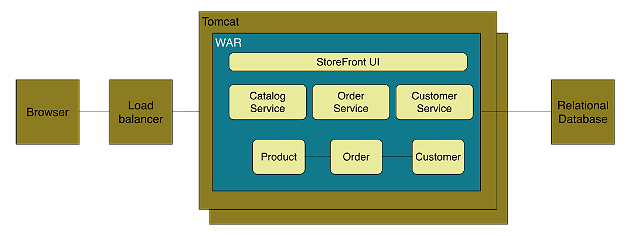
\includegraphics[width=0.8\textwidth]{figures/context-monolith-example}
\caption{Monolith Example from \cite{Richardson:2014aa}}
\label{fig:context/monolith-example}
\end{center}
\end{figure}

\subsection{Types of Monolith Architecture Style}\label{subsection:context/monolith-types}
According to \cite{Annett:2014aa}, a monolith can be of several types depending upon the viewpoint, as shown below:
\begin{enumerate}
\item Module Monolith: If all the code to realize an application share the same codebase and need to be compiled together to create a single artifact for the whole application then the architecture is Module Monolith Architecture. An example is show in figure \ref {fig:context/module-monolith-example}. The application on the left has all the code in the same codebase in the form of packages and classes without clear definition of modules and get compiled to a single artifact. However, the application on the right is developed by a number of modular codebase, each has separate codebase and can be compiled to different artifact. The modules uses the produced artifacts which is different than the earlier case where the code referenced each other directly.
\begin{figure}[H]
\begin{center}
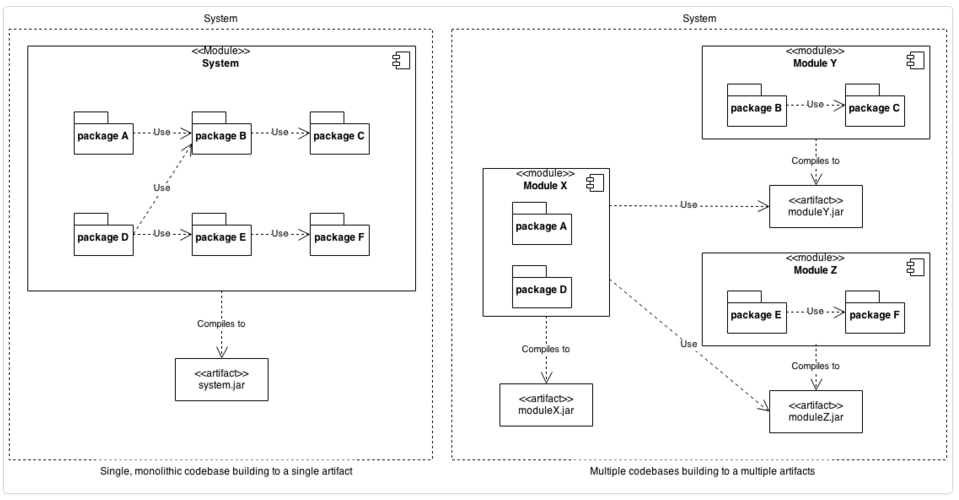
\includegraphics[width=0.8\textwidth]{figures/context-module-monolith}
\caption{Module Monolith Example from \cite{Annett:2014aa}}
\label{fig:context/module-monolith-example}
\end{center}
\end{figure}
\\
\item Allocation Monolith: An Allocation Monolith is created when all code is deployed to all the servers as a single version. This means that all the components running on the servers have the same versions at any time. The figure \ref{fig:context/allocation-monolith-example} gives an example of allocation monolith. The system on the left have same version of artifact for all the components on all the servers. It does not make any differenct whether or not the system has single codebase and artifact. However, the system on the right as shown in the figure is realized with multiple version of the artifacts in different servers at any time.
\begin{figure}[H]
\begin{center}
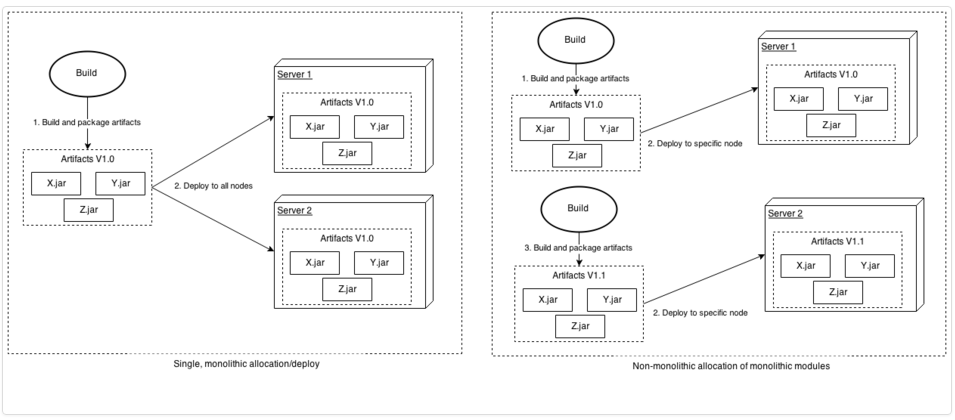
\includegraphics[width=0.8\textwidth]{figures/context-allocation-monolith}
\caption{Allocation Monolith Example from \cite{Annett:2014aa}}
\label{fig:context/allocation-monolith-example}
\end{center}
\end{figure}
\\
\item Runtime Monolith: In Runtime Monolith, the whole application is run under a single process. The left system in the figure \ref{fig:context/runtime-monolith-example} shows an example of runtime monolith where a single server process is responsible for whole application. Whereas the system on the left has allocated multiple server process to run distinct set of component artifacts of the application.
\begin{figure}[H]
\begin{center}
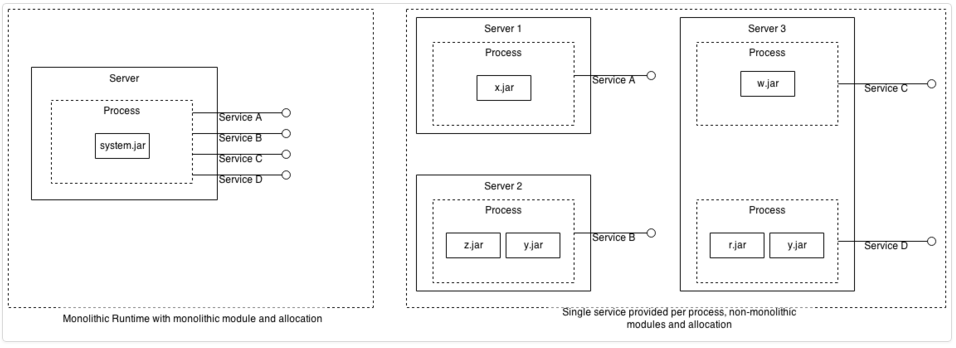
\includegraphics[width=0.8\textwidth]{figures/context-runtime-monolith}
\caption{Runtime Monolith Example from \cite{Annett:2014aa}}
\label{fig:context/runtime-monolith-example}
\end{center}
\end{figure}
\end{enumerate}

\\
\subsection{Advantages of Monolith Architecture Style}\label{subsection:context/monolith-advantages}
The Monolith architecture is appropriate for small application and has following benifits:\cite{Richardson:2014ab}\cite{Fowler:2014aa}\cite{Gupta:2015aa}\cite{Abram:2014aa}
\begin{itemize}[leftmargin=.5in]
\item It is easy to develop a monolith application since various development tools including \acrshort{IDE}s are created around the single application concept. Nevertheless, it is also easy to test the application by creating appropriate environment on the developer's machine.
\item The deployment can be simply achieved by moving the single artifact for the application to an appropriate directory in the server.
\item The scaling can be clearly and easily done by replicating the application horizontally across multiple servers behind a load balancer as shown in figure \ref{fig:context/monolith-example}
\item The different teams are working on the same codebase so sharing the functionality can be easier.
\end{itemize}
\\
\subsection{Disadvantages of Monolith Architecture Style}\label{subsection:context/monolith-disadvantages}
As the requirement grows with time, alongside as application becomes huge and the size of team increases, the monolith architecture faces many problems. Most of the advantages of monolith architecture for small application will not be valid anymore. The challenges of monolith architecture for such agile and huge context are as given below:\cite{Namiot:2014aa}\cite{Newman:2015aa}\cite{Abram:2014aa}\cite{Richardson:2014aa}\cite{Richardson:2014ab}\cite{Gupta:2015aa}
\begin{itemize}[leftmargin=.5in]
\item Limited Agility: As the whole application has single codebase, even changing a small feature to release it in production takes time. Firstly, the small change can also trigger changes to other dependent code because in huge monolith application it is very difficult to manage modularity especially when all the team members are working on the same codebase. Secondly, to deploy a small change in production, the whole application has to be deployed. Thus continuous delivery gets slower in case of monolith application. This will be more problematic when multiple changes have to be released on a daily basis. The slow pace and frequency of release will highly affect agility.
\\
\item Decrease in Productivity: It is difficult to understand the application especially for a new developer because of the size. Although it also depends upon the structure of the codebase, it will still be difficult to grasp the significance of the code when there is no hard modular boundary.Additionally, the developer can be intimidated due to need to see the whole application at once from outwards to inwards direction. Secondly, the development environment can be slow to load the whole application and at the same time the deployment will also be slow. So, in overal it will slow down the speed of understandability, execution and testing.
\\
\item Difficult Team Structure: The division of team as well as assigning tasks to the team can be tricky. Most common ways to partition teams in monolith are by technology and by geography. However, each one cannot be used in all the situations. In any case, the communication among the teams can be difficult and slow. Additionally, it is not easy to assign vertical ownership to a team from particular feature from development to relase. If something goes wrong in the deployment, there is always a confusion who should find the problem, either operations team or the last person to commit. The approprate team structure and ownership are very important for agility.
\\
\item Longterm Commitment to Technology stack: The technology to use is chosen before the development phase by analysing the requirements and the maturity of current technology at that time. All the teams in the architecture need to follow the same techonology stack. However, if the requirement changes then there can be situation when the features can be best soloved by different sets of technology. Additionally, not all the features in the application are same so cannot be treated accordingly in terms of technology as well. Nevertheless, the technology advances rapidly. So, the solution thought at the time of planning can be outdated and there can be a better solution available. In monolith application, it is very difficult to migrate to new technology stack and it can be rather painfull process.
\\
\item Limited Scalability: The scalability of monolith application can be done in either of two ways. The first way is to replicate the application along many servers and dividing the incoming request using a load balancer in front of the servers. Another approach is using the identical copies of the application in multiple servers as in previous case but partitioning the database access instead of user request. Both of these scaling approaches improves the capacity and availability of the application. However, the individual requirement regarding scaling for each component can be different but cannot be fulfilled with this approach. Also, the complexity of the monolith application remains the because we are replicating the whole application. Additionally, if there is a problem in a component the same problem can affect all the servers running the copies of the application and does not improve resilency.\cite{MacVittie:2014aa}\cite{Namiot:2014aa}
\end{itemize}

\section{Decomposition of Application}\label{section:context/decompostion-of-application}
The section \ref{subsection:context/monolith-disadvantages} specified various disadvantages related to monolith architecture style. The book \cite{Fisher:2015aa} provides a way to solve most of the discussed problems such as agility, scalability, productivity etc. It provides three dimensions of scalability as shown in figure \ref{fig:context/scale-cube} which can be applied alone or simultaneously depending upon the situation and desired goals.

\begin{figure}[H]
\begin{center}
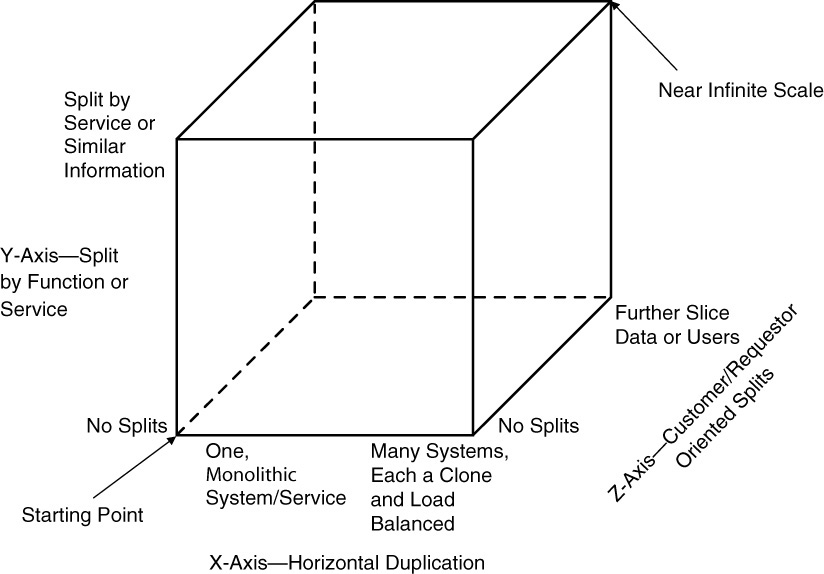
\includegraphics[width=0.8\textwidth]{figures/context-scale-cube}
\caption{Scale Cube from \cite{Fisher:2015aa}}}
\label{fig:context/scale-cube}
\end{center}
\end{figure}

\\
The scaling along each dimensions are described below. \cite{Fisher:2015aa}\cite{MacVittie:2014aa}\cite{Richardson:2014aa}
\begin{enumerate}
\item X-axis Scaling: It is done by cloning the application and data along multiple servers. A pool of requests are applied into a load balancer and the requests are deligated to any of the servers. Each of the server has the full capability of the application and full access to all the data required so in this respect it does not make any difference which server fulfills the request. Rather, it is about how many requests are fulfilled at any time. It is easy to scale along X-axis as the number of requests increases. The solution is as simple as to add additional clones. However, with this type of scaling, it is not scale with the increase in data. Moreover, it also does not scale when there are large variation in the frequency of any type of requests or there dominant requests types because all the requests are handled in an unbiased way and allocated to servers in the same way.
\\
\item Z-axis Scaling: The scaling is done by spliting the request based on certain critera or information regarding the requestor or customer affected by the request. It is different than X-axis scaling in the way that the servers are responsible for different kinds of requests. Normally, the servers have same copy of the application but some can have additional functionalies depending upon the requests expected. The Z-axis scaling helps in fault isolation and transaction scalability. Using this scaling, certain group of customers can be given added functionality or a new functionality can be tested to a small group and thus minimizing the risk.
\\
\item Y-axis Scaling: The scaling along this dimension means the spliting of the application responsibility. The separation can be done either by data, by the actions performed on the data or by combination of both. The respective ways can be referred to as resoure-oriented or service-oriented splits. While the x-axis or z-axis split were rather duplication of work along servers, the y-axis is more about specialization of work along servers. The major advantage of this scaling is that each request is scaled and handled differently according to its necessity. As the logic along with the data to be worked on are separated, developers can focus and work on small section at a time. This will increase productivity as well as agility. Additionally, a fault on a component is isolated and can be handled gracefully without affecting rest of the application. However, scaling along Y-axis can be costly compared to scaling along other dimensions.
\end{enumerate}



\section{Microservice Architecture Style}\label{section:context/microservices_architecture_style}
The section \ref{subsection:context/monolith-disadvantages} listed various disadvantages of following monolithic architecture style especially when the application grows in size rapidly. To counteract those issues, the section \ref{section:context/decompostion-of-application} proposed a way of using scale-cube to decompose the application into individual features, each feature being scaled individually. The same approach is utilized by Microservice Architecture Style, in which an application is decomposed into various individual components, each component runs in a separate process and can be deployed as well as scaled individually.
\\
There are several definitions given by several pioneers and early adapters of the style.
\\
\begin{shaded}Definition 1: \cite{Richardson:2014ac} \end{shaded}
"It is the way to functionally decompose an application into a set of collaborating services, each with a set of narrow, related functions, developed and deployed independently, with its own database."

\\
\begin{shaded}Definition 2: \cite{Wootton:2014aa}\end{shaded}
"It is a style of software architecture that involves delivering systems as a set of very small, granular, independent collaborating services."


\\
\begin{shaded}Definition 3: \cite{Cockcroft:2015aa}\end{shaded}
"Microservice is a loosely coupled Service-Oriented Architecture with bounded contexts."


\\
\begin{shaded}Definition 4: \cite{Fowler:2014aa}\cite{Radchenko:2015aa}\end{shaded}
"Microservices are Service-Oriented Architecture done right."


\\
\begin{shaded}Definition 5: \cite{Fowler:2014aa}\end{shaded}
" Microservice architecture style is an approach to developing a single application as a suite of small services, each running in its own process and communicating with lightweight mechanisms, often an HTTP resource API. These services are built around business capabilities and independently deployable by fully automated deployment machinery. There is a bare minimum of centralized management of these services, which may be written in different programming languages and use different data storage technologies."
\\
\\
\\
The authors have their own way of interpretation of microservices but at the same time agree upon some basic concepts regarding the architecture. However, each definition can be used to understand different aspect of the microservices. A distinct set of keywords can be identified which represents different aspects pointed by the authors and various concepts they agree. Moreover, the table lists important keywords. These keywords provide us some hint regarding various topics of discussion related to microservices, which are listed in columns. Finally, understanding these keywords can be one of the approaches to understand microservices architecture and answer various questions.

\begin{table}[h!]
  \centering
  \begin{adjustbox}{max width=\textwidth}
  \begin{tabular}{*{14}{|c}|}%%{|c|c|c|c|c|c|}
  \hline
  \# & keywords & size & Quality of good microservice & communication & process to create microservices\\
  \hline
  \hline
   1 & Collaborating Services                                       &   &   & \checkmark &  \\ \hline
   2 & Communicating with lightweight mechanism like http           &   &   & \checkmark &  \\ \hline
   3 & Loosely coupled, related functions                           &   & \checkmark  & \checkmark &   \\ \hline
   4 & Developed and deployed independently       &  &   &  & \checkmark \\ \hline
   5 & Own database                                 &  & \checkmark &  & \checkmark \\ \hline
   6 & Different database technologies         &  &  &  & \checkmark \\ \hline
   7 & Service Oriented Architecture  & & \checkmark &  & \checkmark \\ \hline
   8 & Bounded Context  & \checkmark & \checkmark &  & \checkmark \\ \hline
   9 & Build around Business Capabilities  & \checkmark & \checkmark &  &\checkmark \\ \hline
   10 & Different Programming Languages & &  & & \checkmark \\ \hline
   \hline
   \end{tabular}
\end{adjustbox}
  \caption{Keywords extracted from various definitions of Microservice}
  \label{tab:context/microservices_architecture_style/keywords_extracted_from_various_definitions_of_microservice}
\end{table}
%comment from Manoj
\begin{comment}
Start with the properties of microservices and not directly Granularity? May be if we had talked about the qualities of microservices, it would have made more sense.
\end{comment}
%comment from Andrea
\begin{comment}
- compare the 'dimension by interface' and 'dimension by realization', and provide which should be considered
- define efficiency and reuse efficiency
- create a table to show what are good and bad services vs your goal and case.
- use common understandable term for 'volume' of service, either 'size'
\end{comment}
%To be done
\begin{comment}
- factors influencing size of a service such as single responsibility principle, technology, bounded context, autonomy
\end{comment}


\chapter{Granularity}\label{chapter:granularity}
\section{Introduction}\label{section:granularity/introduction}
The granularity of a service is often ambiguous and has different interpretation. In simple term, it refers to the size of the service. However, the size itself can be vague. It can neither be defined as a single quantitative value nor it can be defined in terms of single dependent criterion. It is difficult to define granularity in terms of number because the concepts defining granularity are vague and subjective in nature. If we choose an activity supported by the service to determine its granularity then we cannot have one fixed value instead a hierarchical list of answers; where an activity can either refer to a simple state change, any action performed by an actor or a complete business process. \cite{Linthicum:2015aa}, \cite{Raf-Haesen:2015aa}
\\
Although, the interest upon the granularity of a component or service for the business users only depends upon their business value, there is no doubt that the granularity affects the architecture of a system. The honest granularity of a service should reflect upon both business perspective and should also consider the impact upon the overall architecture.
\\
If we consider other units of software application, we come from object oriented to component based and then to service oriented development. Such a transistion has been considered with the increase in size of the individual unit. The increase in size is contributed by the interpretation or the choice of the abstraction used. For example, in case of object oriented paradigm, the abstraction is chosen to represent close impression of real world objects, each unit representing fine grained abstraction with some attributes and functionalities. 
\\
Such abstraction is a good approach towards development simplicity and understanding, however it is not sufficient when high order business goals have to be implemented. It indicates the necessity of coarser-grained units than units of object oriented paradigm. Moreover, component based development introduced the concept of business components which target the business problems and are coarser grained. The services provide access to application where each application is composed of various component services. \cite{Linthicum:2015aa}


\section{Related Work}\label{section:granularity/relatedwork}

A number of researches have been done in the area of service and component granularity. The focus of the researches includes various areas such as definition, effect, its dependent criteria and various measurement metrics.
\\
According to \cite{Padmal-Vitharana:2004aa}, the granularity of a component is inversely related to various non functional qualities such as customization and maintainaibility.
\\
According to Hazen and Sims \cite{Peter-Herzum:2000aa}, component granularity is rather recursive as a component can be composed of various fine-grained components. They further classify recursion as of discrete or continuous nature but then prefer on discrete recursion. Thus, component granularity can be divide into three discrete layers: system, business and distributed where the composition happens from right to left order and granularity decreases in the opposite order.
It is also useful to relate granularity with reusability. Coarse-grained components have high reuse efficiency because they are well focused to a specific business functionality. Whereas fine-grained components have high reusability since they focus on small functionality and thus can be used by other coarse-grained components to accomplish higher level business capabilities. \cite{Hafedh-Mili:2001aa}, \cite{Zhongjie-Wang:2005aa}
\\
Additionally, Sims \cite{Sims:2005aa} gave some insights to measure granularity. The granularity can be measured either a) by the number of components called from an operation on a service interface, b) by the number of components calling the service interface or c) by the number of database tables updated.
\\
Service Oriented Architecture Framework (\acrshort{SOAF} \cite{Abdelkarim-Erradi:2006aa} also gives some way to measure the granularity in terms of quantitative value. The value can be derived from a) the number of components that are invoked by the service interface and b) the number of changes of states in resources like the database tables updates influenced by the service. Again, the granularity can affect reusability and the network communication to accomplish any task. Coarse grained components have more volume of data exchanged where as fine grained components have high frequency of round trips to complete the full business functionality. It is recommended to balance them which can depend upon various factors such as abstraction level, change expectation rate, service complexity, desired coupling and cohesion. Furthermore, the granularity can be at different levels within an application. High-level business process can be realized as a coarse-grained services and each coarse-grained component can be composed of various fine-grained services.
\\
The idea of multi-layered granularity is further supported by Security Trading case study \cite{Abdelkarim-Erradi:2006aa} and International Financial and Brokerage Services \acrshort{IFBS} case study \cite{Naveen-Kulkarni:2008aa}. The design of pilot application for Security Trading consists of various services across various levels such as process, application, shared data and infrastructures and containing services with granularity decreasing from left to the right in the order they are listed. The application for IFBS is refactored from large number of fine-grained service to multi-layered granular services such as process services, business services, composite services or orchestration services, utility services etc.
\\
A research performed by Steghuis \cite{Steghuis:2006aa} talks about various aspects of granularity such as functionality, flexibility, reusability, complexity, context-independence, Performance, Genericity and sourcing. Some differenciating aspects in comparision to previous researches are context-independence, genericity and sourcing. Context-independence means independence and self sufficiency in terms of data as well as logic. It promotes loose coupling and insists lack of knowledge of state of surrounding and inessential maintainance of own state. Genericity is the quality of making generic services which can be used in different situations such as messaging service. Finally, sourcing is the process of identifying cohesive group of tasks which can be outsourced by considering the coupling associated.

\section{Basic Principles to Service Granularity}\label{section:granularity/principles}
In addition to quantitative perspective on granularity, it can be helpful to approach the granularity qualitatively. The points below are some basic principls derived from various scientific and research papers, which attempt to define the qualitative properties of granularity. Hopefully, these principles will be helpful to come with the service of right granularity.

\begin{enumerate}
\item The correct granularity of a component or a service is dependent upon the time. The various supporting technologies that evolve during time can also be an important factor to define the level of vertical decomposition. For eg: with the improvement in virtualization, containerization as well as platform as a service technologies, it is fast and easy for deployment automation which supports multiple fine-grained services creation.\cite{Peter-Herzum:2000aa}

\item A good candidate for a service should be independent upon the implementation but should depend upon the understandability of domain experts.

\cite{Raf-Haesen:2015aa, Peter-Herzum:2000aa}
\item A service should be an autonomous reusable component and should support various cohesion such as functional (group similar functions), temporal(change in the service should not affect other services), run-time(allocate similar runtime environment for similar jobs; eg. provide same address space for jobs of similar computing intensity) and actor (a component should provide service to similar users).
\cite{Raf-Haesen:2015aa}, \cite{Peter-Herzum:2000aa}

\item A service should not support huge number of operations. If it happens, it will affect high number of customers on any change and there will be no unified view on the functionality. Furthermore, if the interface of the service is small, it will be easy to maintain and understand.\cite{Raf-Haesen:2015aa}, \cite{Pierre-Reldin:2007aa}

\item A service should provide transaction integrity and compensation. The activities supported by a service should be within the scope of one transaction. Additionally, the compensation should be provided when the transaction fails. If each operation provided by the service map to one transaction, then it will improve availability and fault-recovery. \cite{Raf-Haesen:2015aa}, \cite{Foody:2005aa} \cite{Bianco:2007aa}

\item The notion of right granularity is more important than that of fine or coarse. It depends upon the usage condition and moreover is about balancing various qualities such as reusability, network usage, completeness of context etc. \cite{Raf-Haesen:2015aa}, \cite{Lawrence-Wilkes:2004aa}

\item The level of abstraction of the services should reflect the real world business activities. Doing so will help to map business requirements and technical capabilities. \cite{Pierre-Reldin:2007aa}

\item If there are ordering dependencies between the operations, it will be easy to implement and test if the dependent operations are all combined into a single service. \cite{Bianco:2007aa}

\item There can be two better approaches for breaking down an abstraction. One way is to separate redundant data or data with different semanting meaning. The other approach is to divide services with limited control and scope. For example: A Customer Enrollment service which deals with registration of new customers and assignment of unique customer ID can be divided into two independent fine-grained services: Customer Registration and ID Generation, each service will have limited scope and separate context of Customer.\cite{Pierre-Reldin:2007aa}

\item If there are functionalities provided by a service which are more likely to change than other functionalities. It is better to separate the functionality into a fine-grained service so that any further change on the functionality will affect only limited number of consumers. \cite{Bianco:2007aa}
 
\end{enumerate}

\section{Dimensions of Granularity}\label{section:granularity/dimensions}
As already mentioned in \ref{section:granularity/introduction}, it is not easy to define granularity of a service quantitatively. However, it can be made easier to visualize granularity if we can project it along various dimensions, where each dimension is a qualifying attribute responsible for illustrating size of a service. Eventhough the  dimensions discussed in this section will not give the precise quantity to identify granularity, it will definitely give the hint to locate the service in granularity space. It will be possible to compare the granularity of two distinct services. Moreover, it will be interesting and beneficial to know how these dimensions relate to each other to define the size.

\subsection{Dimension by Interface}\label{subsection:granularity/dimensions/interface}
One way to define granularity is by the perception of the service interface as made by its consumer. The various properties of a service interface responsible to define its size are listed below.
\begin{enumerate}
\item Functionality: It qualifies the amount of functionality offered by the service. The functionality can be either default functionality, which means some basic group of logic or operation provided in every case. Or the functionality can be parameterized and depending upon some values, it can be optionally provided. Depending upon the functionality volume, the service can be either fine-grained or course-grained than other service. Considering functionality criterion, A service offering basic CRUD functionality is fine-grained than a service which is offers some accumulated data using orchestration. \cite{Raf-Haesen:2015aa}
\\
\item Data: It refers to the amount of data handled or exchanged by the service. The data granularity can be of two types. The first one is input data granularity, which is the amount of data consumed or needed by the service in order to accomplish its tasks. And the other one is ouput data granularity, which is the amount of data returned by the service to its consumer. Depending upon the size and quantity of business object/objects consumed or returned by the service interface, it can be coarse or fine grained. Additionally, if the business object consumed is composed of other objects rather than primitive types, then it is coarser-grained. For example: the endpoint "PUT customers/C1234" is coarse-grained than the endpoint "PUT customers/C1234/Addresses/default" because of the size of data object expected by the service interface. \cite{Raf-Haesen:2015aa}
\\
\item Business Value: According to \cite{Rolland:2015aa}, each service is associated with an intention or business goal and follows some strategy to achiee that goal. The extent or magnitude of the intention can be perceived as a metric to define granularity. A service can be either atomic or aggregate of other services which depends upon the level of composition directly influenced by the extent of target business goal. An atomic service will have lower granularity than an aggregate in terms of business value. For example, sellProduct is coase-grained than acceptPayment, which is again coarse-grained than validateAccountNumber. \cite{Raf-Haesen:2015aa}
\end{enumerate}

\subsection{Dimension by Interface Realization}\label{subsection:granularity/dimensions/interface_realization}
The section \ref{subsection:granularity/dimensions/interface} provides the aspect of granularity with respect to the perception of customer to interface. However, there can be different opinion regarding the same properties, when it is viewed regarding the imlementation. This section takes the same aspects of granularity and try to analyze them when the services are implemented.
\begin{enumerate}
\item Functionality: In section \ref{subsection:granularity/dimensions/interface}, it was mentioned that an orchestration service has higher granularity than its constituent services with regard to default functionality. If the realization effort is focused, it may only include compositional and/or compensation logic because the individual tasks are acomplshed by the constituent service interfaces. Thus, in terms of the effort in realizing the service it is fine-grained than from the view point of interface by consumer. \cite{Raf-Haesen:2015aa}
\\
\item Data: In some cases, services may utilize standard message format. For example: financial services may use \acrshort{SWIFT} for exchanging finanicial messages. These messages are extensible and are coarse grained in itself. However, all the data accepted by the service along with the message may not be required and used in order to fulfil the business goal of the service. In that sense, the service is coarse-grained from the viewpoint of consumer but is fine-grained in realization point of view. \cite{Raf-Haesen:2015aa}
\\
\item Business Value: It can make a huge impact when analyzing business value of service if the realization of the service is not considered well. For example: if we consider data management interface which supports storage, retrieval and transaction of data, it can be considered as fine-grained because it will not directly impact the business goals. However, since other services are very dependent in its performance, it becomes necessary to analyse the complexity associated with the implementation, reliablity and change the infrastructure if needed. These comes with additional costs, which should well be analyzed. From the realization point of view, the data service is coarse-grained than its view by consumer. \cite{Raf-Haesen:2015aa}
\end{enumerate}

\begin{framed}
\textbf{\textit{Principle: A high Functionality granularity does not necessarily mean high business value granularity}}
\\
It may seem to have direct proportional relationship between functionality and business value granularity. The business value of a service reflects business goals however the functionality refers to the amount of work done by the service. A service to show customer history can be considered to have high functionality granularity because of the involved time period and database query. However, it is of very low business value to the enterprise. \cite{Raf-Haesen:2015aa}
\end{framed}


\subsection{R\textsuperscript{3} Dimension}\label{subsection:granularity/dimensions/r3}
Keen \cite{Keen:2015aa} and later  Weill and Broadbent \cite{Weill:1998aa} introduced a separate group of criteria to measure granularity of service. The granularity was evaluated in terms of two dimensions as shown in the Figure \ref{fig:Reach-Range Model}

\begin{figure}[H]
\begin{center}
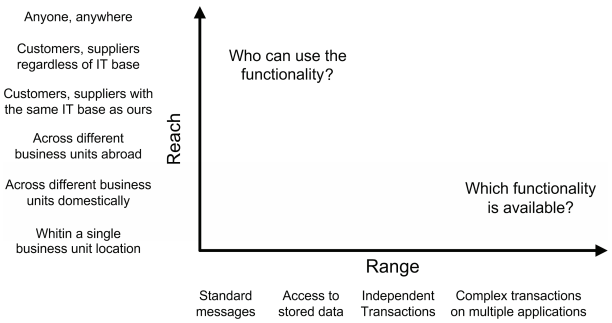
\includegraphics[width=0.8\textwidth]{figures/Granularity-R3-one}
\caption{Reach and Range model from \cite{Keen:2015aa, Weill:1998aa}}
\label{fig:Reach-Range Model}
\end{center}
\end{figure}

Reach: It provides various levels to answer the question “Who can use the functionality? ”.  It provides the extent of consumers, who can access the functionality provide  by the service. It can be a customer, the customers within an organization, supplier etc. as given by the Figure \ref{fig:Reach-Range Model}.
\\
Range: It gives answer to “Which functionality is available? ”. It shows the extent to which the information can be accessed from or shared with the service. The levels of information accessed are analyzed depending upon the kind of business activities accessible from the service. It can be a simple data access, a transaction, message transfer etc as shown in the Figure \ref{fig:Reach-Range Model} The 'Range' measures the amount of data exchanged in terms of the levels of business activities important for the organization. One example for such levels of activities with varying level of 'Range' is shown in Figure \ref{fig:Range Example}.
\begin{figure}[H]
\begin{center}
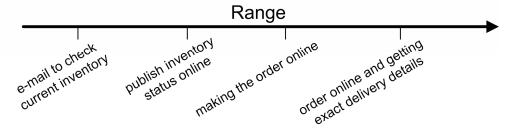
\includegraphics[width=0.8\textwidth]{figures/Granularity-R3-two}
\caption{Example to show varying Range from \cite{Keen:2015aa, Weill:1998aa}}
\label{fig:Range Example}
\end{center}
\end{figure}
In the figure \ref{fig:Range Example}, the level of granularity increases as the functionality moves from 'accessing e-mail message' to 'publishing status online' and then to 'creating order'. It is due to the change in the amount of data access involved in each kind of functionality. Thus, the 'Range' directly depends upon the range of data access.
\\
As the service grows,  alongside 'Reach' and 'Range' also peaks up, which means the extent of consumers as well as the kind of functionality increase. This will add complexity in the service. The solution proposed by \cite{Cockburn:2001aa} is to divide the architecture into services. However, only 'Reach' and 'Range' will not be enough to define the service. It will be equally important to determine scope of the individual services. The functionality of the service then should be define in two distinct dimensions 'which kind of functionality' and 'how much functionality'. This leads to another dimension of service as described below.
\cite{Keen:2015aa, Weill:1998aa, Pierre-Reldin:2007aa}
\\
Realm: It tries to create a boundary around the scope of the functionality provided by the service and thus clarifies the ambiguity created by 'Range'. If we take the same example as given by Figure \ref{fig: Range Example}, the range alone defining the kind of functionaly such as creating online order does not explicitly clarifies about what kind of order is under consideration. The order can be customer order or sales order. The specification of 'Realm' defining what kind of order plays role here. So, we can have two different services each with same 'Reach' and 'Range' however different 'Realm' for customer order and Sales order.  \cite{Keen:2015aa, Weill:1998aa, Pierre-Reldin:2007aa}

The consideration of all aspects of a service including 'Reach', 'Range' and 'Realm' give us a model to define granularity of a service and is called R\textsuperscript{3} model. The volume in the R\textsuperscript{3} space for a service gives its granularity. A coarse-grained service has higher R\textsuperscript{3} volume then fine-grained service. The figures \ref{fig:R3 volume-granularity analogy greater}  and \ref{fig:R3 volume-granularity analogy equal} show such volume-granularity analogy given by R\textsuperscript{3} model. \cite{Keen:2015aa, Weill:1998aa, Pierre-Reldin:2007aa}

\begin{figure}[H]
\begin{center}
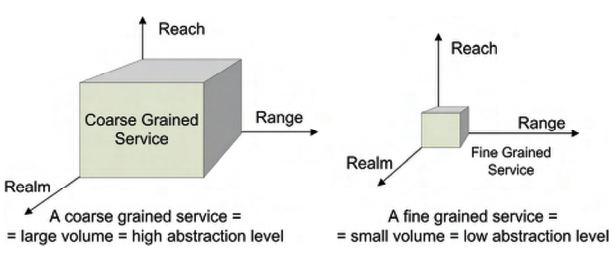
\includegraphics[width=0.8\textwidth]{figures/Granularity-R3-three}
\caption{R\textsuperscript{3} Volume-Granularity Analogy to show direct dependence of granularity and volume \cite{Pierre-Reldin:2007aa}}
\label{fig:R3 volume-granularity analogy greater }
\end{center}
\end{figure}

\begin{figure}[H]
\begin{center}
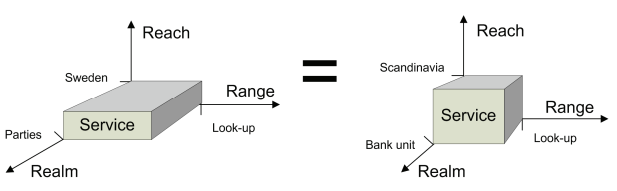
\includegraphics[width=0.8\textwidth]{figures/Granularity-R3-four}
\caption{R\textsuperscript{3} Volume-Granularity Analogy to show same granularity with different dimension along axes \cite{Pierre-Reldin:2007aa}}
\label{fig:R3 volume-granularity analogy equal}
\end{center}
\end{figure}


\subsection{Retrospective}\label{subsection:granularity/dimensions/retrospective}
The sections \ref{subsection:granularity/dimensions/interface} and \ref{subsection:granularity/dimensions/interface_realization} classified granularity of a service along three different directions: data, functionality and business value. Moreover, the interpretation from the viewpoint of interface by consumer and the viewpoint of producer for realization were also made.
Again, the section \ref{subsection:granularity/dimensions/r3} divides the aspect of granularity along Reach, Range and Realm space, the granularity given by the volume in the R\textsuperscript{3} space.
Despite of good explanation regarding each aspect, the classification along data, functionality and business value do not provide discrete metrics to define granularity in terms of quantitatively. However, the given explanations and criteria are well rounded to compare two different services regarding granularity. These can be effectively used to classify if a service is fine-grained than other service.
The R\textsuperscript{3} model in section \ref{subsection:granularity/dimensions/r3} additionally provides various levels of granularity along each axis. This makes it easy to at least measure the granularity and provides flexibility to compare the granularity between various services.
\\
A case study \cite{Pierre-Reldin:2007aa} using data, functionality and business criteria to evaluate the impact of granularity on the complexity in the architecture is held. The study was done at KBC Bank & Insurance Group of central Europe. Along the study, the impact of each kind of granularity is verified. The important results fromt the study are listed below.

\begin{enumerate}
\item A coarse-grained service in terms of 'Input Data' provides better transactional support, little communication overhead and also helps in scalability. However, there is a chance of data getting out-of-date quickly.
\item A coarse-grained service in terms of 'Output Data' also provides good communication efficiency and supports reusability.
\item A fine-grained service along 'Default Functionality' has high reusability and stability but low reuse efficiency.
\item A coarse-grained service due to more optional functionalities has high reuse efficiency, high reusability and also high stability but the implementation or realization is complicated.
\item A coarse-grained service along 'Business Value' has high consumer satisfaction value and emphasize the architecturally crucial points fulfilling business goals.
\end{enumerate}

Similarly, a study was carried out in Handelsbanken in sweden, which has been working with Service-Oriented architecture. The purpose of the study was to analyze the impact of R\textsuperscript{3} model on the architecture. It is observed that there are different categories of functionalities essential for an organization. Some functionality can have high Reach and Range with single functionality and other may have complex functionality with low Reach and Range. The categorization and realization of such functionalities should be accessed individually. It is not necessary to have same level of granularity across all services or there is no one right volume for all services. However, if there are many services with low volume, then we will need many services to accomplish a high level functionality. Additionally, it will increase interdependency among services and network complexity. Finally, the choice of granularity is completely dependent upon the IT-infrastructure of the company. The IT infrastructure decides which level of granularity it can support and how many of them. \cite{Pierre-Reldin:2007aa}


\begin{framed}
\textbf{\textit{Principle: IT-infrastructure of an organization affects granularity.}} \label{principle:granularity/IT_infrastructure}
\\
The right value of granularity for an organization is highly influenced by its IT infrastructure. The organization should be capable of handling the complexities such as communication, runtime, infrastructure etc if they choose low granularity. \cite{Pierre-Reldin:2007aa}
\end{framed}

Additionally, it is observed that a single service can be divided into number of granular services by dividing across either Reach, Range or Realm. The basic idea is to make the volume as low as possible as long as it can be supported by IT-infrastructure. Similarly, each dimension is not completely independent from other. For example: If the reach of a service has to be increased from domestic to global in an organization then the realm of the functionality has to be decreased in order to make the volume as low as possible, keep the development and runtime complexities in check. \cite{Pierre-Reldin:2007aa}

\begin{framed}
\textbf{\textit{Principle: Keep the volume low if possible.}}
\\
If supported by IT-infrastructure, it is recommended to keep the volume of service as low as possible, which can be achieved by managing the values of Reach, Range and Realm. It will help to decrease development and maintenance overload. \cite{Pierre-Reldin:2007aa}
\end{framed}


\begin{comment}
An additional contribution to defining the granularity has been made when the differentiating features of distributed system are taken into consideration. The granularity of a service depends upon the coupling and cohesion. In order to find the right granularity for a service, we need to balance between coupling and cohesion.
The coupling can be determined from the dependency graph between a service and its consumers. The goal is to minimize the coupling of individual service and to the application as a whole.
The cohesion is evaluated by the likeliness of the operations supported by the service. It considers that higher the similarities among the operations, higher the cohesion is.  \cite{Xiao-jun:2015aa}, \cite{Mikhail-Perepletchikov:2015aa}, \cite{Bingu-Shim:2008aa}

Service Hierarchy
\end{comment}

 
%comment from Manoj
\begin{comment}
try to reference ISO/IEC 9126 for the quality attributes: refer to the slides sent by Manoj on Nov 02
Also include the formula of the metrics and discuss about them and simplify them: refer to the slides sent by Manoj on Nov 02
The quality attributes which can make more sense according to the priority to microservices: refer to the slides sent by Manoj on Nov 02
Relationship between the quality attributes and their tradeoffs, what happens when we try to increase cohesion.. how it affect other attributes?
create wiki page in the sebis page to document the literature review.
\end{comment}

\%comment from Andrea
\begin{comment}
mention about coupling created by calling same database directly by multiple microservice
use the formula to calculate quality metrics for the services at hybris to give an idea about good and bad service, the process of finding out good service at first and then using the quality metrics finding out the range of quality metrics, which can then be used to identify bad services
\end{comment}



\chapter{Quality of Service}\label{chapter:quality_of_service}

\section{Introduction}\label{section:quality_of_service/introduction}
In addition to allign with the business requirements, an important goal of software engineering is to provide high quality. The quality assessment in the context of service oriented product becomes more crucial as the complexity of the system is getting higher by time. \cite{Zhang:2009aa, Goeb:2011aa, Nematzadeh:2014aa} Quality models have been devised over time to evaluate quality of a software. A quality model is defined by quality attributes and quality metrics. Quality attributes are the expected properties of software artifacts defined by the chosen quality model. And, quality metrics give the techniques to measure the quality attributes. \cite{Mancioppi:2015aa} The software quality attributes can again be categorized into two types: internal and external attributes. \cite{Mancioppi:2015aa, Briand:1996aa} The internal quality attributes are the design time attributes which should be fulfilled during the design of the software. Some of the external quality attributes are loose coupling, cohesion, granularity, autonomy etc.\cite{Rostampour:2011aa, Sindhgatta:2015aa, Elhag:2014aa} On the other hand, the external quality attributes are the traits of the software artifacts produced at the end of Software Development Life Cycle \acrshort [{SDLC}]. Some of them are reusability, maintainability etc. \cite{Elhag:2014aa, Mancioppi:2015aa, Feuerlicht:2007aa, Feuerlicht:2013aa} For that reason, the external quality attributes can only be measure after the end of development. However, it has been evident that internal quality attributes have huge impact upon the value of external quality attributes and thus can be used to predict them. \cite{Henry:1990aa, Briand:2015aa, Alshayeb:2003aa, Bingu-Shim:2008aa}The evaluation of both internal and external quality attributes are valuable in order to produce high quality software.\cite{Mancioppi:2015aa, Perepletchikov:2007aa, Mikhail-Perepletchikov:2015aa}

\section{Quality Attributes}\label{section:quality_of_service/quality_attributes}
As already mentioned in section \ref{section:quality_of_service/introduction}, the internal and external qualities determine the overall value of the service composed. There are different researches and studies which have been performed to find the features affecting the service qualities. Based on the published research papers, a comprehensive table \ref{tab:quality_of_service/quality_attributes} has been created. The table provides a minimum list of quality attributes which have been considerd in various research papers. 

  \begin{table}[h!]
  \centering
  \begin{adjustbox}{max width=\textwidth}
  \begin{tabular}{*{14}{|c}|}%%{|c|c|c|c|c|c|c|c|}
  \hline
  \# & Attribute & \cite{Sindhgatta:2015aa} & \cite{Xiao-jun:2015aa} & \cite{Saad-Alahmari:2011aa} & \cite{Bingu-Shim:2008aa} & \cite{Ma:2009aa} & \cite{Feuerlicht:2007aa}\\
  \hline
  \hline
   1 & Coupling & \checkmark & \checkmark & \checkmark & \checkmark & \checkmark & \checkmark\\ 
   2 & Cohesion & \checkmark & X & \checkmark & \checkmark & \checkmark & \checkmark\\
   3 & Autonomy & \checkmark & X & X & X & X & X\\
   4 & Granularity & \checkmark & \checkmark & \checkmark & \checkmark & \checkmark & \checkmark\\
   5 & Reusability & \checkmark & X & X & \checkmark & X & \checkmark\\
   6 & Abstraction & \checkmark & X & X & X & X & X\\
   7 & Complexity & X & X & X & \checkmark & X & X\\
  \hline
\end{tabular}
\end{adjustbox}
  \caption{Quality Attributes}
  \label{tab:quality_of_service/quality_attributes}
\end{table}

The table \ref{tab:quality_of_service/quality_attributes} gives a picture of the studies done so far around service quality attributes. It can be deduced that most of the papers focus on coupling and granularity of the service and only few of them focus on other attributes such as complexity and autonomy.

Coupling refers to the dependency and interaction among services. The interaction becomes inevitable when a service requires a functionality provided by another service in order to accomplish its own goals. Similarly, Cohesion of any system is the extent of appropriate arrangement of elements to perform the functionalities. It affects the degree of understandability and sensibility of its interface for its consumers. Whereas, the complexity attribute provides the way to evaluate the difficulty in understanding and reasoning the context of the service or component.\cite{Elhag:2014aa}
\\
The reusability attribute for a service measures the degree to which it can be used by multiple consumer services and can undergo multiple composition to accoplish various high order functionalities. \cite{Feuerlicht:2007aa}
\\
Autonomy is a broad term which refers to the ability of a service for self-containment, self-controlling, self-governance. Autonomy defines the boundary and context of the service. \cite{Ma:2007aa} Finally, granularity is described in chapter \ref{chapter:granularity} in detail. The basic signifance of granularity is the diversity and size of the functionalities offered by the service. \cite{Elhag:2014aa}

\section{Quality Metrics}\label{section:quality_of_service/quality_metrics}
There have been many studies made to define metrics for quality components.A major portion of the research have been done for object oriented and component based development. These metrics are refined to be used in service oriented systems.\cite{Xiao-jun:2015aa, Sindhgatta:2015aa} Firslty, various papers related to quality metrics of service oriented systems are collected. The papers which conducted their findings or proposition based on quality amount of scientific studies and have produced convincing result are only selected.  Additionally, the evaluation presented in the research papers were only done using the case studies of their own and not real life scenarios. Furthermore, they have used diversity of equations to define the quality metrics. On the basis of case studies made in the papers only, a fair comparision and choice of only one way to evaluate the quality metrics cannot be made. This is further added by the fact that the few papers cover most of the quality metrics, most of them focus on only few quality metrics such as coupling but not all of them focus on all the quality metrics. Nevertheless, they do not discuss about the relationship between all quality metrics. \cite{Elhag:2014aa} This creates difficulty to map all the quality metrics into a common calculation family. 
\\
With such situation, this section will focus on facilitating the understanding of the metrics. Despite the case that there is no idea of threshold value of metrics discussed to define the optimal quality level, the discussed method can still be used to evaualte the quality along various metrics and compare the various design artifacts. This will definitely help to choose the optimum design based on the criteria. Also, there is complexity in understanding and confusion to follow a single proposed metrics procudure. But, the existing procedures can be broken down further to the simple understandable terms. By doing so, the basic terms which are the driving factors for the quality attributes and at the same time followed by most of the procedures as defined in the papers, can be identified.
\\
The remaining part of this section will attempt to collaborate the metrics definitions proposed in various papers, analyze them to identify their conceptual base of measurement in simplest form.

\subsection{Context and Notations}{\label{section:quality_of_service/quality_metrics/context_and_notations}

Before looking into the definitions of metrics, it will help understanding, to know related terms, assumptions and their respective notations. 

\begin{itemize}[leftmargin=.5in]
\item the business domain is realized with various processes defined as $ P = \{p_1, p_2...p_s \} $
\item a set of services realizing the application is defined as $ S = \{s_1, s_2...s_s \} $; $s_s$ is the total number of services in the application
\item for any service $ s \epsilon S$, the set of operations provided by s is given by $O(s) = \{o_1, o_2,...o_o\}$ and $ |O(s)| $ = O
\item if an operation $ o \epsilon O(s) $ has a set of input and output messages given by M(o). Then the set of messages of all operations of the service is given by $ M(s) = \cup_{o \epsilon O(s)} M(o)$
\item the consumers of the service $ s \epsilon S $ is given by $ S_{consumer}(s) = \{ S_{c1}, S_{2},...S{{n_c}\}$; $n_c$ gives the number of consumer services
\item the producers for the service or the number of services to which the given service $ s \epsilon S $ is dependent upon is given by $ S_{producer}(s) = \{ S_{c1}, S_{2},...S{{n_p}\}$; $n_p$ gives the number of producer services
\end{itemize}

\\
%coupling metrics
\subsection{Coupling Metrics}{\label{section:quality_of_service/quality_metrics/coupling}

\cite{Sindhgatta:2015aa} defines following metrics to determine coupling
$$ \acrshort{SOCI}(s) = number\_of\_operations\_invoked $$ $$ = | \{ o_{i} \epsilon s_{i}: \exists_{o \epsilon s} calls(o, o_{i}) \wedge s \neq s_{i} \} | $$

$$ \acrshort{ISCI}(s) = number\_of\_services\_invoked $$ $$ = | \{ s_{i} : \exists_{o \epsilon s}, \exists_{o_{i} \epsilon s_{i}} calls(o, o_{i}) \wedge s \neq s_{i} \} | $$

$$ \acrshort{SMCI}(s) = size\_of\_message\_required\_from\_other\_services $$ $$ = | \cup M (o_{i}) : ( o_{i} \epsilon s_{i}) \vee ( \exists_{o \epsilon s}, \exists_{o_{i} \epsilon s_{i} } calls(o, o_{i}) \wedge s \neq s_{i} ) | $$

where, \\
\begin{itemize}[leftmargin=.5in]
\item SOCI is Service Operation Coupling Index
\item ISCI is Inter Service Coupling Index
\item SMCI is Service Message Coupling Index
\item $ call(o, o_i) $ represents the call made from service 'o' to service '$o_i$'
\end{itemize}
\\
\cite{Xiao-jun:2015aa} defines 
$$Coupling(S_i) =  p \sum_{j=1}^{n_s} (-log(P_L(j)))$$
$$= \frac{1}{n} \sum_{j=1}^{n_s} (-log(P_L(j)))$$

where, \\
\begin{itemize}[leftmargin=.5in]
\item $n_s$ is the total number of services connected
\item 'n' is the total number of services in the entire application
\item $p = \frac{1}{n}$ gives the probability of a service participating in any connection
\end{itemize}
\\
\cite{Kazemi:2011aa} defines
$$Coupling = \frac{dependency\_on\_business\_entities\_of\_other\_services}{number\_of\_operations\_and\_ dependencies}$$ $$=\frac{\sum_{i \epsilon D_s} \sum_{k \epsilon O(s)}CCO(i,k)}{|O(s)|.K}$$
where, \\
\begin{itemize}[leftmargin=.5in]
\item $D_s = \{ D_1, D_2,...D_k \}$ is set of dependencies the service has on other services
\item $ K = |D_s| $
\item CCO is Conceptual Coupling betweeen service operations and obtained from BE X EBP (CRUD) matrix table constructed with business entities and business operations, where BE is business entity and EBP any logical process defined in an operation.
\end{itemize}

\cite{Bingu-Shim:2008aa} defines
$$coupling(s) =  \frac{number\_of\_services\_connected}{number\_of\_services} $$ $$ =\frac{n_c + n_p}{n_s}$$
where, \\
\begin{itemize}[leftmargin=.5in]
\item $n_c$ is number of consumer services
\item $n_p$ number of dependent services
\item $n_s$ total number of services
\end{itemize}
\cite{Saad-Alahmari:2011aa} defines
$$coupling = \frac{number\_of\_invocation}{number\_of\_services}$$ $$=\frac{\sum_{i=1}^{|O(s)|} (S_{i,sync} + S_{i,async})}{|S|}$$
\\
where,
\\
\begin{itemize}[leftmargin=.5in]
\item $S_{i,sync}$ is the synchronous invocation in the operation $O_i$
\item $S_{i,async}$ is the asynchronous invocation in the operation $O_i$
\end{itemize}


\begin{table}[h]
  \centering
  \begin{adjustbox}{max width=\textwidth}
  \normalsize
  \begin{tabular}{*{14}{|c}|}%%{|c|c|l|}
  \hline
  \# & Papers & Metrics Definition \\
  \hline
  \hline
   1 & \cite{Sindhgatta:2015aa} & 
                    \begin{tabular}{cl}
                    \multirow{6}{*}
                    &\acrshort{SOCI} : number of operation of other services \\
                    &invoked by the given service\\
                    &\acrshort{ISCI} : number of services invoked \\
                    &by a given service\\
                    &\acrshort{SMCI} : total number of messages from \\
                    &information model required by the operations\\
                    \end{tabular}\\
                    \hline
   2 & \cite{Xiao-jun:2015aa} &
                    \begin{tabular}{cl}
                    \multirow{6}{*}
                    &Coupling is evaluated as information entropy \\
                    &of a complex service\\
                    &component where entropy is calculated using various \\
                    &data such as total number of atomic components connected, \\
                    &total number of links to atomic \\ 
                    &components and total number of atomic components\\
                    \end{tabular}\\
                    \hline
   3 & \cite{Kazemi:2011aa} & 
                    \begin{tabular}{cl}
                    \multirow{7}{*}
                    &The coupling is measured by using the dependency \\
                    &of a service operations with operations of other \\
                    &services. Additionally, the dependency is considered \\
                    &to have different weight value for each kind of operation \\
                    &such as Create, Read, Update, Delete (CRUD) and based on \\
                    &the type of business entity involved. The weight is \\
                    &referred from the CRUD matrix constructed in the process.\\
                    \end{tabular}\\
                    \hline
   4 & \cite{Bingu-Shim:2008aa} & 
                    given by the average number of directly connected services\\
  \hline
   5 & \cite{Saad-Alahmari:2011aa} & 
                    \begin{tabular}{cl}
                    \multirow{2}{*}
                    &defines coupling as the average number of synchronous and \\
                    &asynchronous invocations in all the operations of the service\\
                    \end{tabular}\\
                    \hline
\end{tabular}
\end{adjustbox}
  \caption{Coupling Metrics}
  \label{tab:quality_of_service/quality_attributes/coupling_metrics}
\end{table}
\\
The table \ref{tab:quality_of_service/quality_attributes/coupling_metrics} shows simpler form of metrics proposed for coupling. Although, the table shows different way of evaluating coupling, they somehow agree to the basic metrics to calculate coupling. It can be deduced that the metrics to evaluate coupling uses basic metrics such as number of operations, number of provider services and number of messages.
\\

%cohesion metrics
\subsection{Cohesion Metrics}{\label{section:quality_of_service/quality_metrics/cohesion}

\cite{Sindhgatta:2015aa} defines following metric for cohesion.
$$ \acrshort{SFCI}(s) = \frac{number\_of\_operations\_using\_same\_message}{number\_of\_operations} $$ $$ = \frac{max (\mu(m) )}{|O(s)|} $$
\\
where,
\begin{itemize}[leftmargin=.5in]
\item SFCI is Service Functional Cohesion Index
\item the number of operations using a message 'm'  is $\mu(m)$ such that $ m \epsilon M(s) $ and |O(s)| > 0
%principle
\\The service is considered highly cohesive if all the operations use one common message. This implies that a higly cohesive  service operates on a small set of key business entities as guided by the messages and are  relavant to the service and all the operations operate on the same set of key business entities. \cite{Sindhgatta:2015aa}
\end{itemize}

\cite{Bingu-Shim:2008aa} defines
$$ cohesion =  \frac{n_s}{|M(s)|}$$

\cite{Perepletchikov:2007aa} defines

$$ \acrshort{SIDC} = \frac{number\_of\_operations\_sharing\_same\_parameter}{total\_number\_of\_parameters\_in\_service} $$ $$ = \frac{ n_{op} }{n_{pt}} $$

$$ \acrshort{SIUC} = \frac{sum\_of\_number\_of\_operations\_used\_by\_each\_consumer}{product\_of\_total\_no\_of\_consumers\_and\_operations} $$ $$= \frac{n_{oc}}{n_c * |O(s)|}$$

$$ SSUC = \frac{sum\_of\_number\_of\_sequentials\_operations\_accessed\_by\_each\_consumer}{product\_of\_total\_no\_of\_consumers\_and\_operations} $$ $$=\frac{n_{so}}{n_c * |O(s)|}$$

\\where,
\begin{itemize}[leftmargin=.5in]
\item SIDC is Service Interface Data Cohesion
\item SIUC is Service Interface Usage Cohesion
\item SSUC is Service Sequential Usage Cohesion
\item $n_{op}$ is the number of operations in the service which share the same parameter types
\item $n_{pt}$ is the total number of distinct parameter types in the service
\item $n_{oc}$ is the total number of operations in the service used by consumers
\item $n_{so}$ is the total number of sequentially accessed operations by the clients of the service
\end{itemize}
\cite{Saad-Alahmari:2011aa} defines
$$ cohesion = \frac{max(\mu(\acrshort{OFG}, \acrshort{ODG}))}{|O(s)|} $$

\\
where,
\\
\begin{itemize}[leftmargin=.5in]
\item \acrshort{OFG} and \acrshort{ODG} are Operation Gunctionality Granularity and Operation Data Granularity respectively as calculated in section \ref{section:quality_of_service/quality_metrics/granularity}
\item $\mu(\acrshort{OFG}, \acrshort{ODG})$ gives the number of operations with specific value of \acrshort{OFG} and \acrshort{ODG}
\end{itemize}

\begin{table}[h]
  \centering
  \begin{adjustbox}{max width=\textwidth}
  \begin{tabular}{*{14}{|c}|}%%{|c|c|l|}
  \hline
  \# & Papers & Metrics Definition \\
  \hline
  \hline
   1 & \cite{Sindhgatta:2015aa} & 
                    \begin{tabular}{cl}
                    \multirow{3}{*}
                    &defines \acrshort{SFCI} which measures the fraction of operations \\
                    &using similar messages out of total  number of operations in the \\
                    &service operations of the service\\
                    \end{tabular}\\
                    \hline
   2 & \cite{Perepletchikov:2007aa} &
                    \begin{tabular}{cl}
                    \multirow{8}{*}
                    &\acrshort{SIDC} : defines cohesiveness as the fraction of operations \\
                    &based on commonality of the messages they operate on\\
                    &\acrshort{SIUC} : defines the degree of consumption pattern of \\
                    &the service operations which is based on the similarity of consumers\\
                    &of the operations\\ 
                    &\acrshort{SSUC} : defines the cohesion based on the sequential\\
                    &consumption behavior of more than one operations of a service by\\
                    &other services\\
                    \end{tabular}\\
                    \hline
   3 & \cite{Bingu-Shim:2008aa} & 
                    \begin{tabular}{cl}
                    \multirow{2}{*}
                    &cohesion is given by the inverse of average number of consumed \\
                    &messages by a service\\
                    \end{tabular}\\
                    \hline
   4 & \cite{Saad-Alahmari:2011aa} & 
                    \begin{tabular}{cl}
                    \multirow{4}{*}
                    &cohesion is defined as the consensus among the operations of \\
                    &the service regarding the functionality and data granularity \\
                    &which represents the type of parameters and the operations \\
                    &importance as calculated in the section
                    \ref{section:quality_of_service/quality_metrics/granularity}\\
                    \end{tabular}\\
                    \hline
\end{tabular}
\end{adjustbox}
  \caption{Cohesion Metrics}
  \label{tab:quality_of_service/quality_attributes/cohesion_metrics}
\end{table}
\\
The table \ref{tab:quality_of_service/quality_attributes/cohesion_metrics} gives simplified view for the cohesion metrics. The papers presented agree on some basic metrics such as similarity of the operation usage behavior, commanility in the messages consumed by operations and similarity in the size of operations.
\\


%granularity metrics
\subsection{Granularity Metrics}{\label{section:quality_of_service/quality_metrics/granularity}

\cite{Sindhgatta:2015aa} defines
$$ \acrshort{SCG} = number\_of\_operations = |O(s)| $$ 
$$ \acrshort{SDG} = size\_of\_messages =|M(s)| $$
where,
\begin{itemize}[leftmargin=.5in]
\item SCG is Service Capability Granularity
\item SDG is Service Data Granularity
\end{itemize}

\cite{Bingu-Shim:2008aa} defines
$$ granularity = \frac{number\_of\_operations}{size\_of\_messages} = \frac{|O(s)|^2}{|M(s)|^2}$$

\cite{Saad-Alahmari:2011aa} defines

$$ ODG = fraction\_of\_total\_weight\_of\_input\_and\_output\_parameters $$ $$ = \bigg( \frac{ \sum_{i=1}^{n_io} W_{pi}}{ \sum_{i=1}^{n_is} W_{pi}} + \frac{\sum_{j=1}^{n_jo} W_{pj}}{ \sum_{j=1}^{n_js} W_{pj}} \bigg)$$

$$ OFG = complexity\_weightage\_of\_operation = \frac{W_i(o)}{ \sum_{i=1}^{|O(S)|}W_i(o)}$


$$ granularity = sum\_of\_product\_of\_data\_and\_functionality\_granularity $$ $$= \sum_{i=1}^{|O(S)|} ODG(i) * OFG(i) $$
\\
where,
\\
\begin{itemize}[leftmargin=.5in]
\item ODG is Operation Data Granularity
\item OFG is Operation Functionality Granularity
\item $W_{pi}$ is the weight of input parameter
\item $W_{pj}$ is the weight of output parameter
\item $n_io$ is the number of input parameters in an operation
\item $n_jo$ is the number of output parameters in an operation
\item $n_is$ is the total number of input parameters in the service
\item $n_js$ is the total number of output parameters in the service
\item $W_i(o)$ is the weight of an operation of the service
\item $ |O(S)| $ is the number operations in the service
\end{itemize}

\begin{table}[h!]
  \centering
  \begin{adjustbox}{max width=\textwidth}
  \begin{tabular}{*{14}{|c}|}%%{|c|c|l|}
  \hline
  \# & Papers & Metrics Definition \\
  \hline
  \hline
   1 & \cite{Sindhgatta:2015aa} & 
                    \begin{tabular}{cl}
                    \multirow{3}{*}
                    &the service capability granularity is given by the number of\\
                    &operations in a service and the data granularity by the\\ 
                    &number of messages consumed by the operations of the service\\
                    \end{tabular}\\
                    \hline
   2 & \cite{Saad-Alahmari:2011aa} &
                    \begin{tabular}{cl}
                    \multirow{8}{*}
                    &\acrshort{ODG} : evaluated in terms of number of input and\\
                    &output parameters and their type such as simple,\\ 
                    &user-defined and complex\\
                    &\acrshort{OFG} : defined as the level of logic provided by\\
                    &the operations of the services\\
                    &\acrshort{SOG} : defined by the sum of product of data \\
                    &granularity and functionality granularity for all operations\\
                    &in the service\\
                    \end{tabular}\\
                    \hline
   3 & \cite{Bingu-Shim:2008aa} & 
                    \begin{tabular}{cl}
                    \multirow{3}{*}
                    &evaluated as the ratio of squared number of operations of\\
                    &the service to the squared number of messages consumed by\\ 
                    &the service\\
                    \end{tabular}\\
                    \hline
\end{tabular}
\end{adjustbox}
  \caption{Granularity Metrics}
  \label{tab:quality_of_service/quality_attributes/granularity_metrics}
\end{table}
\\
The table \ref{tab:quality_of_service/quality_attributes/granularity_metrics} presents various view of granularity metrics based on different research papers. The chapter \ref{chapter:granularity} discuss in detail regarding the topic. Based on the table \ref{tab:quality_of_service/quality_attributes/granularity_metrics}, the granularity is evaluated using some basic metrics such as the number and type of the parameters, number of operations and number of messages consumed.
\\

%Complexity metrics
\subsection{Complexity Metrics}{\label{section:quality_of_service/quality_metrics/complexity}

\cite{Zhang:2009aa} defines
$$ \acrshort{RIS} = \frac{IS(s_i)}{|S|}$$
\acrshort{RCS}
\\

$$  complexity = \frac{coupling\_of\_service}{number\_of\_services} = \frac{CS(s_i)}{|S|}$$

\\
where,
\\
\begin{itemize}[leftmargin=.5in]
\item $CS(s_i)$ gives coupling value of a service
\item |S| is the number of services to realize the application
\item $IS(s_i)$ gives importance weight of a service in an application
\end{itemize}

The complexity is rather given by relative coupling than by coupling on its own. A low value of RCS indicates that the coupling is lower than the count of services where as RCS with value 1 indicates that the coupling is equal to the number of services. This represents high amount of complexity.
\\
Similarly, a high value of RIS indicates that a lot of services are dependent upon the service and the service of critical value for them. This increases complexity as any changes or problem in the service affects a large number of services to a high extent.
\\
\cite{Saad-Alahmari:2011aa} defines
$$ Complexity(s) = \frac{Service\_Granularity}{number\_of\_services} $$ $$ =\frac{\sum_{i=1}^{|O(s)|}(SG(i))^2}{|S|}$$
\\
where,
\\
\begin{itemize}[leftmargin=.5in]
\item |S| is the number of services to realize the application
\item SG(i) gives the granularity of ith service 
\\calculated as described in section \ref{section:quality_of_service/quality_metrics/granularity}
\end{itemize}

refer to the document for effect of RCS and RIS on complixity

\begin{table}[h!]
  \centering
  \begin{adjustbox}{max width=\textwidth}
  \begin{tabular}{*{14}{|c}|}%%{|c|c|l|}
  \hline
  \# & Papers & Metrics Definition \\
  \hline
  \hline
   1 & \cite{Zhang:2009aa} & 
                    \begin{tabular}{cl}
                    \multirow{6}{*}
                    &\acrshort{RCS} : complexity given by the degree of coupling\\ 
                    &for a service and evaluated as the fraction of its coupling\\
                    &to the total number of services\\
                    &\acrshort{RIS} : measured as the fraction of total \\
                    &dependency weight of consumers upon the service to the total\\
                    &number of services\\
                    \end{tabular}\\
                    \hline
   2 & \cite{Saad-Alahmari:2011aa} & 
                    \begin{tabular}{cl}
                    \multirow{2}{*}
                    &the complexity is calculated using the granunarity of service\\
                    &operations\\
                    \end{tabular}\\
  \hline
\end{tabular}
\end{adjustbox}
  \caption{Complexity Metrics}
  \label{tab:quality_of_service/quality_attributes/complexity_metrics}
\end{table}
\\
The table \ref{tab:quality_of_service/quality_attributes/complexity_metrics} provides the way to interprete complexity metrics. The complexity is highly dependent upong coupling and functionality granularity of the service.
\\
%Autonomy metrics
\subsection{Autonomy Metrics}{\label{section:quality_of_service/quality_metrics/autonomy}
\cite{Rostampour:2011aa} defines

$$ Self-Containment (SLC) = sum\_of\_CRUD\_coefficients\_for\_each\_Business\_entity $$ $$ =\frac{1}{h_2 - l_2 + 1} \sum_{i= l_2}^{h_2} \sum_{sr \epsilon SR} (BE_{i,sr} X V_{sr})$$


$$ Dependency (DEP) = dependency\_of\_service\_on\_other\_service\_business\_entities $$ $$ =\frac{\sum_{j=L1_i}^{h1_i} \sum_{k=1}^{BE} V_{sr_{jk}} - \sum_{j=L1_i}^{h1_i} \sum_{k=L2_i}^{j2_i} V_{sr_{jk}} }{nc}$$

$$
\mbox{autonomy}=\left\{
\begin{array}{rl}
\acrshort{SLC} - \acrshort{DEP} & \mbox{if SLC > DEP} \\
0 & \mbox{otherwise}
\end{array} \right.
$$

\\
where,
\\
\begin{itemize}[leftmargin=.5in]
\item nc is the number of relations with other services
\item $BE_{i,sr} = 1$ if the service performs action sr on the ith BE and sr represents any CRUD operation and $V_{sr}$ is the coefficient depending upon the type of action
\item $ V_{sr_{jk} $ is the corresponding value of the action in jkth element of CRUD matrix, it gives the weight of corresponding business capability affecting a business entity
\item $ l1_i, h1_i, l2_i, h2_i$ are bounding indices in CRUD matrix of ith service
\end{itemize}
 
\begin{table}[h!]
  \centering
  \begin{adjustbox}{max width=\textwidth}
  \begin{tabular}{*{14}{|c}|}%%{|c|c|l|}
  \hline
  \# & Papers & Metrics Definition \\
  \hline
  \hline
   1 & \cite{Rostampour:2011aa} & 
                   \begin{tabular}{cl}
                    \multirow{6}{*}
                    &\acrshort{SLC} : defined as the degree of control of a \\
                    &service upon its operations to act on its Business entities only\\
                    &\acrshort{DEP} : given by the degree of coupling of the given \\
                    &service with other services\\
                    &autonomy is given by the difference of \acrshort{SLC} and \acrshort{DEP}\\
                    &if SLC > DEP else it is taken as 0\\
                    \end{tabular}\\
                    \hline
\end{tabular}
\end{adjustbox}
  \caption{Autonomy Metrics}
  \label{tab:quality_of_service/quality_attributes/autonomy_metrics}
\end{table}
\\
The table \ref{tab:quality_of_service/quality_attributes/autonomy_metrics} shows a way to interprete autonomy. It is calculated by the difference \acrshort{SLC}-\acrshort{DEP} when \acrshort{SLC} is greater than \acrshort{DEP}. In other cases it is taken as zero. So, autonomy increases as the operations of the services have full control upon its business entities but decreases if the service is dependent upon other services.
\\
%Reusability metrics
\subsection{Reusability Metrics}{\label{section:quality_of_service/quality_metrics/reusability}
\cite{Sindhgatta:2015aa} defines

$$ Reusability = number\_of\_existing\_consumers $$ $$ =|S_{consumers}| $$
%P + Q $$ where,
%$$ P = | \{ s_{i} : \exists_{o \epsilon s} , \exists_{o_{i} \epsilon s_{i}} calls(o_{i}, o) \wedge s \neq %s_{i}} \}|$$ and
%$$ Q = |\{ p \epsilon P : s \epsilon p \}|$$

\\ \cite{Bingu-Shim:2008aa} defines 
$$Reusability= \frac{Cohesion - granularity + Consumability - coupling}{2}$$
\begin{table}[h!]
  \centering
  \begin{adjustbox}{max width=\textwidth}
  \begin{tabular}{*{14}{|c}|}%%{|c|c|l|}
  \hline
  \# & Papers & Metrics Definition \\
  \hline
  \hline
   1 & \cite{Sindhgatta:2015aa} & 
                    \begin{tabular}{cl}
                    \multirow{2}{*}
                    &\acrshort{SRI} defines reusability as the number of existing\\ 
                    &consumers of the service\\
                    \end{tabular}\\
                    \hline
   2 & \cite{Bingu-Shim:2008aa} & 
                    \begin{tabular}{cl}
                    \multirow{4}{*}
                    &evaluated from coupling, cohesion, granularity and \\
                    &consumability of a service where consumability is the chance \\
                    &of the service being discovered and depends upon the fraction\\
                    &of operations in the service\\
                    \end{tabular}\\
                    \hline
                    \end{tabular}
\end{adjustbox}
  \caption{Reusability Metrics}
  \label{tab:quality_of_service/quality_attributes/reusability_metrics}
\end{table}
\\
The table \ref{tab:quality_of_service/quality_attributes/reusability_metrics} shows the reusability metrics evaluation. Reusability depends upon coupling, cohesion and granularity. It decreases as coupling and granularity increases.
\\


%Basic Metrics
\section{Basic Quality Metrics}{\label{section:quality_of_service/basic_quality_metrics}
The section \ref{section:quality_of_service/quality_metrics} presents various metrics to evaluate quality attributes based upon different papers. Additionally, the section analyzed the metrics and tried to derive them in simplest form possible. Eventually, the tables demonstrating the simplest definition of the metrics shows that the different quality attributes are measured on the basis of some basic metrics. Based on the section \ref{section:quality_of_service/quality_metrics} and based on the papers, this section will attempt to derive basic metrics.
\\

\begin{table}[h!]
  \centering
  \begin{adjustbox}{max width=\textwidth}
  \begin{tabular}{*{14}{|c}|}%%{|c|l|c||c||c||c||c||c|}
  \hline
  \# & Metrics & \begin{sideways}Coupling\end{sideways}
  &  \begin{sideways}Cohesion\end{sideways}
  & \begin{sideways}Granularity\end{sideways}
  & \begin{sideways}Complexity\end{sideways} 
  & \begin{sideways}Autonomy\end{sideways}
  & \begin{sideways}Reusability\end{sideways} \\
  \hline
  \hline
    1 & number of service operations invoked by the service 
     & +
     & 
     & 
     & +
     & -
     & -\\
                    \hline
    2 & number of operation using similar messages
     & 
     & +
     & 
     & 
     & 
     & +\\
\hline
    3 & number of operation used by same consumer
     & 
     & +
     & 
     & 
     & 
     & +\\
     \hline
    4 & number of operation using similar parameters
     & 
     & +
     & 
     & 
     & 
     & +\\
     \hline
    5 & number of operation with similar scope or capability
     & 
     & +
     & 
     & 
     & 
     & +\\
     \hline
    6 & scope of operation
     & 
     & 
     & +
     & +
     & 
     & -\\
     \hline
     7 & number of operations
     & 
     & 
     & +
     & +
     & 
     & -\\
     \hline
     8 & number of parameters in operation
     & 
     & 
     & +
     & +
     & 
     & -\\
     \hline
    9 & type of parameters in operation
     & 
     & 
     & +
     & +
     & 
     & -\\
     \hline
     10 & number and size of messages used by operations
     & +
     & 
     & +
     & +
     & -
     & -\\
     \hline
     11 & type of messages used by operations
     & 
     & +
     & 
     & 
     & 
     & +\\
     \hline
     12 & number of consumer services
     & +
     & 
     & 
     & +
     & -
     & +\\
     \hline
     13 & number of producer services
     & +
     & 
     & 
     & +
     & -
     & -\\
     \hline
     14 & type of operation and business entity invoked by the service
     & +
     & 
     & 
     & +
     & -
     & -\\
     \hline
     15 & number of consumers accessing same operation
     & 
     & +
     & 
     & 
     & 
     & +\\
     \hline
     16 & number of consumer with similar operation usage sequence
     & 
     & +
     & 
     & 
     & 
     & +\\
     \hline
     17 & dependency degree or imporance of service operation to other service
     & 
     & 
     & 
     & +
     & 
     & \\
     \hline
     18 & degree of control of operation to its business entities
     & 
     & 
     & 
     & 
     & +
     & \\
     \hline
     \hline
\end{tabular}
\end{adjustbox}
  \caption{Basic Quality Metrics}
  \label{tab:quality_of_service/quality_attributes/basic_quality_metrics}
  \\
  Moreover, the effect of the basic metrics upon various quality attributes are also evaluated.
  Here, the meaning of the various symbols to demonstrate the affect are as given below:
  \\
\begin{itemize}[leftmargin=.5in]
\item + the basic metric affect the quality attribute proportionlly
\item - the basic metric inversely affect the quality attribute
\item   there is no evidence found regarding the relationship from the papers
\end{itemize}
\end{table}


%principles based on quality quality attributes
\section{Principles defined by Quality Attributes}{\label{section:quality_of_service/quality_attributes_principle}
The section \ref{section:quality_of_service/introduction} has already mentioned that there are two distinct kind of quality attributes: external and internal. The external quality attributes cannot be evaluated during design however can be predicted using the internal quality attributes. This kind of relationship can be used to design service with good quality. Moreover, it is important to identify how each internal attributes affect the external attributes. The understanding of such relationship will be helpful to identify the combined effect of the quality attributes and eventually to identify the service with the appropriate level of quality as per the requirement.
The remaining part of the section lists relationship existing in various quality attributes as well as the desired value of the quality attributes.
\begin{enumerate}
\item When a service has large number of operations, it means it has large number of consumers. It will highly affect maintainability because a small change in the operations of the service will be propagated to large number of consumers. But again, if the service is too fine granular, there will be high network coupling. \cite{Feuerlicht:2007aa, Xiao-jun:2015aa}\cite{Bianco:2007aa}

\item Low coupling improves understandability, reusability and scalability where as high coupling decreases maintainability. \cite{Kazemi:2011aa}\cite{Erl:2005aa}\cite{Josuttis:2007aa}

\item A good strategy for grouping operations to realize a service is to combine the ones those are used together.  This indicates that most of the operations are used by same client.  It highly improves maintainability by limiting the number of affected consumer in the event of any change in the service. \cite{Xiao-jun:2015aa}

\item A high cohesive quality attribute defines a good service. The service is easy to understand, test, change and is more stable. These properties highly support maintainability. {enumerate}\cite{np:2001aa}

\item A service with operations those are cohesive and have low coupling which make the service reusable. \cite{Washizakia:2003aa}\cite{Feuerlicht:2007aa}\cite{Ma:2009aa}

\item Services must be selected in a way so that they focus on a single business functionality. This highly follows the concept of low coupling. \cite{Perepletchikov:2007aa}\cite{Sindhgatta:2015aa}

\item Maintainability is divided into four distinct concepts:  analyzability, changeability, stability and testability.\cite{np:2001aa} A highly cohesive and low-coupled design should be easy to analyze and test. Moreover,  such a system will be stable and easy to change.\cite{Perepletchikov:2007aa}


\item The complexity of a service is determined by granularity. A coarse-grained service has higher complexity. However, as the size of the service decreases, the complexity of the over system governance also increases.
\cite{Saad-Alahmari:2011aa}

\item The complexity depends upon coupling. The complexity of a service is defined in terms of the number of dependencies of a service, number of operations as well as number and size of messages used by the service operations.\cite{Saad-Alahmari:2011aa}\cite{Sindhgatta:2015aa}\cite{Lee:2001aa}

\item The selection of an appropriate service has to deal with multi-objective optimization problem.  The quality attributes are not independent in all aspects. Depending upon goals of the architecture, tradeoffs have to be made for mutually exclusive attributes. For example, when choosing between coarse-grained and fine-grained service, various factors such as governance, high network roundtrip etc. also should be considered. 
\cite{Jamshidi:2008aa}

\item Business entity convergence of a service, which is the degree of control over specific business entities, is an important quality for the selection of service. For example: It is be better to create a single service to create and update an order. In that way change and control over the business entity is localized to a single service.\cite{Ma:2009aa}

\item Increasing the granularity decreases cohesion but also decreases the amount of message flow across the network. This is because, as the boundary of the service increases, more communication is handled within the service boundary. However, this can be true again only if highly related operations are merged to build the service. This suggests for the optimum granularity by handling cohesion and coupling in an appropriate level.\cite{Ma:2009aa}\cite{Bianco:2007aa}

\item As the scope of the functionality provided by the service increases, the reusability decreases.
\cite{Feuerlicht:2007aa}

\item If the service has high interface granularity, the operations operates on coarse-grained messages. This can affect the service performance. On the other hand, if the service has too fine-grained interface, then there will be a lot of messages required for the same task, which then can again affect the overall performance. \cite{Bianco:2007aa}


\end{enumerate}


%relationship between quality attributes and tradeoffs
\section{Relationship among Quality Attributes}{\label{section:quality_of_service/quality_attributes_relationship}
In order to determine the appropriate level of quality for a service, it is also important to know the relationship between the quality attributes. This knowledge will helpfull to decide tradeoffs among them in the situation when it is not possible to achieve best of all. Based on the section \ref{section:quality_of_service/quality_attributes} and section \ref{section:quality_of_service/quality_attributes_principle}, the identified relationship among the quality attributes are shown in the table \ref{tab:quality_of_service/quality_attributes/quality_attributes_relationship}.

\begin{table}[h!]
  \centering
  \begin{adjustbox}{max width=\textwidth}
  \begin{tabular}{*{14}{|c}|}%%{|c|c|c|c|c|}
  \hline
  \# & Quality Attributes & Coupling & Cohesion & Granularity \\
  \hline
  \hline
   1 & Coupling         &   & - & + \\ \hline
   2 & Cohesion         & - &   &   \\ \hline
   3 & Granularity      & + &   &   \\ \hline
   4 & Complexity       & + &   & + \\ \hline
   5 & Reusability      & - & + & - \\ \hline
   6 & Autonomy         & - &   &   \\ \hline
   7 & Maintainability  & - & + & - \\ \hline
   \hline
   \end{tabular}
\end{adjustbox}
  \caption{Relationship among quality attributes}
  \label{tab:quality_of_service/quality_attributes/quality_attributes_relationship}
\end{table}

Here, the meaning of the various symbols showing nature of relationship are as given below:
  \\
\begin{itemize}[leftmargin=.5in]
\item + the quality attribute on the column affects the quality attribute on the corresponding row positively
\item - the quality attribute on the column affects the quality attribute on the corresponding row inversely
\item   there is no enough evidence found regarding the relationship from the papers or these are same attributes
\end{itemize}
%where are we on the map ISO/IEC 9126
%quality attrubutes priority for microservices


\chapter{Service Candidate}\label{chapter:service_candidate}

\section{Introduction}\label{section:service_candidate/introduction}
In the previous chapters, granularity and quality of a microservice was focussed. The qualitative as well as quantitative aspects of granularity were described. Additionally, various quality metrics were discussed to measure different quality attributes of a microservce. Moreover, a set of principle guidelines and basic metrics to qualify the microservices were also listed.\\
In addition to that, it is also equally important to agree on the process to identify the service candidates. In this chapter and following chapters, the ways to recognize microservices will be discussed.
There are three basic approaches to identify service candidates: Top-down, bottom-up and meet-in-the-middle. \\
The top-down approach defines the process on the basis of the business model. At first, various models are designed to capture the overall system and architecture. Using the overall design, services are identified upfront in the analysis phase.\\
The next approach is bottom-up, which base its process on the existing architecture and existing application. The existing application is studied to identify the cohesion and consistency of the features provided by various components of the system. This information is used to aggregate the features and identify services in order to overcome the problems in the existing system.\\
Finally, the meet-in-the-middle approach is a hybrid approach of both top-down and bottom-up approaches. In this approach, the complete analysis of system as a whole is not performed upfront as the case of top-down approach. Where as, a set of priority areas are identified and used to analyse their business model resulting in a set of services. The services thus achieved are further analysed critically using bottom-up approach to identify problems. The problems are handled in next iterations where the same process as before is followed. The approach is continued for other areas of the system in the order of their priority.\cite{Pierre-Reldin:2007aa}\cite{Arsanjani:2004aa}

\section{Related Work}\label{section:service_candidate/related_work}
There are various efforts made regarding the identification of service candidates. Among them, most follows top-down approach. Service Oriented Development Architecture (SODA) uses service driven modeling approach to design and implement services.\cite{Nigam:2005aa} Service Oriented Analysis and Design (SOAD) on the other hand uses existing modeling process and notation to desing services. \cite{Arsanjani:2005aa} Service Oriented Unified Process(SOUP) is highly influenced by Rational Unified Process and extreme programming techniques.\cite{Mittal:2005aa}\\
A bottom-up approach Feature Oriented Domain Analysis is also proposed to analysis the existing system features for identifying services.\cite{Kang:1990aa}\\
Among the few meet-in-the-middle approaches is Feature Analysis for Service-Oriented Reengineering which uses business modeling and FODA. \cite{Chen:2005aa} Similarly, Service Oriented Modeling Architecture (SOMA) emphasise on using goal-oriented meet-in-the-middle approach.\cite{Arsanjani:2004aa}\\
Again, there are a majority of papers using use case modeling to identify services. The papers \cite{Millard:2007aa} \cite{Howard:2009aa} defines Service Responsibility and Interaction Design Method (SRI-DM) to utilize use case to identify the service with cohesive set of functionalities. Similarly, the paper \cite{Fareghzadeh:2008aa} identifies various levels of services based on the abstraction level of the use cases.



\chapter{Selection By Use Case}\label{chapter:selection_by_use_case}
\section{Use case}\label{section:selection_by_use_case/use_case}
A use case is an efficient as well as a fancy way of capturing requirements. Another technique of eliciting requirement is by features specification. However, the feature specification technique limits itself to answer only "what the system is intended to do". On the other hand, use case goes further and specifies "what the system does for any specific kind of user". In this way, it gives a way to specify and most importantly validate the expectation and concerns of stakeholders at the very early phase of software development. Undoubtedly for the same reason, it is not just a tool for requirement specification but an important software engineering technique which guides the software engineering cycle. Using use cases, the software can be developed to focus on the concerns that are valueable to the stakeholders and test accordingly.\cite{Ng:2004aa}
\\
It can be valueable to see the ways it has been defined.
\begin{shaded}Definition 1: \cite{Jacobson:1987aa} \end{shaded}
"A use case is a sequence of actions performed by the system to yield an observable result of value to a particular user." 
\\
\begin{shaded}Definition 2: \cite{Rumbaugh:1999aa}\end{shaded}
"A use case is a description of a set of sequences of actions, including variants, that a system performs that yield an observable result of value to an actor."

\section{Use case Refactoring}\label{section:selection_by_use_case/use_case_refactoring}
According to \cite{Jacobson:1987aa} it is not always intuitive to modularize use cases directly. As per the definitions provided in \ref{section:selection_by_use_case/use_case}, a use case consists of a number of ordered functions together to accomplish a certain goal. \cite{Jacobson:1987aa} defines these cohesive functionalites distributed across usecases as clusters. And the process of identifying the clusters scattered around the use cases is the process of identifying services. \cite{Ng:2004aa} and \cite{Jacobson:2003aa} describes use case possibly consisting of various cross-cutting concerns. The papers use the term 'use case module' to define the cohesive set of tasks. The figure \ref{fig:selection_by_use_case/use_case_one} demonstrate the cross cutting functionalities needed by a use case in order to accomplish its goal. For example, the use case 'does A' has to perform separate functionalities on different domain entities X and Y. Similarly, the use case 'does B' needs to perform distinct functions on entities X, Y and Z.
\begin{figure}[H]
\begin{center}
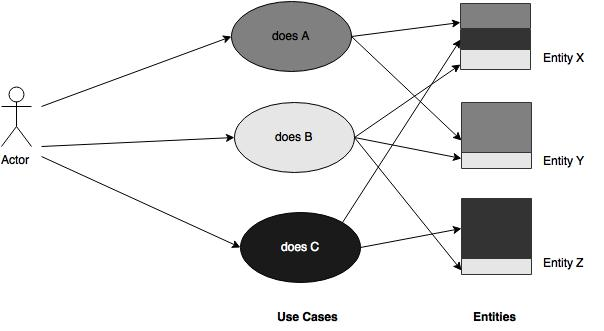
\includegraphics[width=0.8\textwidth]{figures/use-case-one}
\caption{Use cases with cross-cutting concerns \cite{Ng:2004aa}}
\label{fig:selection_by_use_case/use_case_one}
\end{center}
\end{figure}
This situation prompts for the analysis of the use cases for cross cutting tasks and refactoring them in order to map the cohesive functionalities and use cases. Refactoring helps to achieve the right level of abstraction and granularity by improving functionality cohesion as well as elimination of redundancy and finally promoting the reusablity. \cite{Doh:2007aa}
\\
Furthermore, the refactoring is assisted by various relationships in use case model to represent dependencies between use cases, which are include, generalization and extend. \cite{Ng:2004aa}
\\
\section{Process for Use Case Refactoring}\label{section:selection_by_use_case/process_for_use_case_refactoring}
In order to refactor the use cases and finally map use cases to the service, the papers \cite{Kim:2006aa}, \cite{Yun:2006aa} and \cite{Doh:2007aa} provide a comprehensive method. It is a type of meet-in-the-middle approach where use case models are first created and then refactored to create new set of use cases to accomplish high cohesion in functionality and loose coupling. This will ultimately create use cases supporting modularity and autonomy. \cite{Fareghzadeh:2008aa} There are three distinct steps for service identification using service refactoring.
\begin{enumerate}
\item \textbf{TaskTree Generation}\\
In this step, the initial use case model created during domain analysis is used to create task trees for each distinct use case. The task trees provide sequence of individual tasks required to accomplish in order to achieve the goal of the use case.
\\
\item \textbf{Use Case Refactoring}\\
In this step, the task tree generated in the previous step is analysed. As already mentioned in the section \ref{section:selection_by_use_case/use_case_refactoring}, that the initial use case consists of various cross cutting functionalities which runs through large number of business entities. In order to minimize that, refactoring is performed. The detail rules are provided in section \ref{section:selection_by_use_case/rules_for_use_case_refactoring}.
\\
\item \textbf{Service Identification}\\
The use cases achieved after refactoring have correct level of abstractions and granularity representing cohesive business functionality. The unit use cases thus achieved appreciate reuse of common functionality.  \cite{Doh:2007aa} Furthermore, the approach considers the concerns of stakeholders in terms of cohesive business functionalities to be represented by use cases.\cite{Fareghzadeh:2008aa} Additionally, the process also clarifies the dependencies between various use cases. Thus, the final use cases obtained can be directly maped to individual services.
\end{enumerate}
\\
\section{Rules for Use Case Refactoring}\label{section:selection_by_use_case/rules_for_use_case_refactoring}
The context is first defined before distinct rules are presented.
\\
\begin{shaded}Context 1 \end{shaded}
If U represents use case model of the application, $t_i$ represents any task of U and T being the set of tasks of U. Then, $\forall t_i \in T $, $t_i$ exists in the post-refactoring model U'. The refactoring of a use case model preserves the set of tasks.
\\
\begin{shaded}Context 2 \end{shaded}
A refactoring rule R is defined as a 3-tuple (Parameters, Preconditions, Postconditions). Parameters are the entities involved in the refactoring, precondition defines the condition which must be satisfied by the usecase u in order for R to be applied in u. Postcondition defines the state of U after R is applied.
\\
The various refactoring rules are as listed below.
\\
\subsection{Decomposition Refactoring}\label{section:selection_by_use_case/guidelines_for_use_case_refactoring/decomposition_refactoring}
When the usecase is complex and composed of various functionally independent tasks, the tasks can be ejected out of the task tree of the usecase and represented as a new use case. The table \ref{tab:selection_by_use_case/guidelines_for_use_case_refactoring/decomposition_rule} shows the decomposition rule in detail.
\begin{table}[H]
  \centering
  \begin{adjustbox}{max width=\textwidth}
  \begin{tabular}{*{14}{|c}|}%%{|c|l|}
  \hline
  Parameters & 
                    \begin{tabular}{ll}
                    \multirow{3}{*}
                    &u: a use case to be decomposed\\
                    &t: represents task tree of u \\
                    &t': a subtask tree of t\\
                    \end{tabular}\\
                    \hline
   Preconditions  & t' is functionally independent of u \\
                    \hline
   Postconditions &
                    \begin{tabular}{ll}
                    \multirow{2}{*}
                    &1. new use case u' containing task tree t' is generated \\
                    &2. a dependency is created between u and u'\\
                    \end{tabular}\\
                    \hline
\end{tabular}
\end{adjustbox}
  \caption{Decomposition Rule}
  \label{tab:selection_by_use_case/guidelines_for_use_case_refactoring/decomposition_rule}
\end{table}
\\

\subsection{Equivalence Refactoring}\label{section:selection_by_use_case/guidelines_for_use_case_refactoring/equivalence_refactoring}
If the two use cases share their tasks in the task tree, we can conclude that they are equivalent and redundant in the use case model. The table \ref{tab:selection_by_use_case/guidelines_for_use_case_refactoring/equivalence_rule} shows the rule for the refactoring.
\begin{table}[H]
  \centering
  \begin{adjustbox}{max width=\textwidth}
  \begin{tabular}{*{14}{|c}|}%%{|c|l|}
  \hline
  Parameters &  $u_1$ , $u_2$: two distinct use cases\\
                    \hline
   Preconditions  & the task trees of $u_1$ and $u_2$ have same behavior \\
                    \hline
   Postconditions &
                    \begin{tabular}{ll}
                    \multirow{3}{*}
                    &1. $u_2$ is replaced by $u_1$ \\
                    &2. all the relationship of $u_2$ are fulfilled by $u_1$\\
                    &3. $u_2$ has no relationship with any other use cases\\
                    \end{tabular}\\
                    \hline
\end{tabular}
\end{adjustbox}
  \caption{Equivalence Rule}
  \label{tab:selection_by_use_case/guidelines_for_use_case_refactoring/equivalence_rule}
\end{table}
\\

\subsection{Composition Refactoring}\label{section:selection_by_use_case/guidelines_for_use_case_refactoring/composition_refactoring}
When there are two or more small-grained use cases such that they have related tasks, the use cases can be represented by a composite unit use case.

\begin{table}[H]
  \centering
  \begin{adjustbox}{max width=\textwidth}
  \begin{tabular}{*{14}{|c}|}%%{|c|l|}
  \hline
  Parameters & 
                 \begin{tabular}{ll}
                    \multirow{3}{*}
                    & $u_1$, $u_2$: the fine grained use cases\\
                    & $t_1$, $t_2$: the task trees of $u_1$ and $u_2$ respectively\\
                    \end{tabular}\\
                    \hline
   Precondition     & $t_1$ and $t_2$ are functionally related.\\
                    \hline
   Postconditions &
                    \begin{tabular}{ll}
                    \multirow{3}{*}
                    & 1. $u_1$ and $u_2$ are merged to a new unit use case u \\
                    & 2. u has new task tree given by $t_1 \cup t_2 $\\
                    & 3. the dependencies of $u_1$ and $u_2$ are handled by u\\ 
                    & 4. $u_1$ and $u_2$ are deleted along with their task trees $t_1$ and $t_2$\\
                    \end{tabular}\\
                    \hline
\end{tabular}
\end{adjustbox}
  \caption{Composition Rule}
  \label{tab:selection_by_use_case/guidelines_for_use_case_refactoring/composition_rule}
\end{table}
\\

\subsection{Generalization Refactoring}\label{section:selection_by_use_case/guidelines_for_use_case_refactoring/generalization_refactoring}
When multiple use cases share some volume of dependent set of tasks in their task trees, it can be implied that the common tasks set can be represented by a new use case. The table \ref{tab:selection_by_use_case/guidelines_for_use_case_refactoring/generalization_rule} provides the specific of the rule.
\begin{table}[H]
  \centering
  \begin{adjustbox}{max width=\textwidth}
  \begin{tabular}{*{14}{|c}|}%%{|c|l|}
  \hline
  Parameters & 
                 \begin{tabular}{ll}
                    \multirow{2}{*}
                    & $u_1$ , $u_2$: two distinct use cases\\
                    & $t_1$ , $t_2$: task trees of $u_1$ and $u_2$ respectively\\
                    \end{tabular}\\
                    \hline
   Precondition     & $t_1$ and $t_2$ share a common set of task $t= \{ x_1, x_2...x_n \} $\\
                    \hline
   Postconditions &
                    \begin{tabular}{ll}
                    \multirow{5}{*}
                    & 1. a new use case u is created using task tree $t= \{x_1, x_2...x_n \} $ \\
                    & 2. relationship between u with $u_1$  and between u with $u_2$ is created\\
                    & 3. the task tree $t= \{ x_1, x_2...x_n \} $ is removed from task tree of both $u_1$ and $u_2$\\
                    & 4. the common relationship of both $u_1$ and $u_2$ are handled by u and \\ 
                    & removed from them\\
                    \end{tabular}\\
                    \hline
\end{tabular}
\end{adjustbox}
  \caption{Generalization Rule}
  \label{tab:selection_by_use_case/guidelines_for_use_case_refactoring/generalization_rule}
\end{table}
\\


\subsection{Merge Refactoring}\label{section:selection_by_use_case/guidelines_for_use_case_refactoring/merge_refactoring}
When a use case is just specific for another use case and the use case is only the consumer for it, the two use cases can be merged into one.
\begin{table}[H]
  \centering
  \begin{adjustbox}{max width=\textwidth}
  \begin{tabular}{*{14}{|c}|}%%{|c|l|}
  \hline
  Parameters & 
                 \begin{tabular}{ll}
                    \multirow{3}{*}
                    & u, u': the use cases\\
                    & r defines the dependency of u with u'\\
                    & t, t': the task trees of u and u' respectively\\
                    \end{tabular}\\
                    \hline
   Precondition     & there is no dependency of other usecases with u' except u\\
                    \hline
   Postconditions &
                    \begin{tabular}{ll}
                    \multirow{3}{*}
                    & 1. u' is merged to u \\
                    & 2. u has new task tree given by $t \cup t' $\\
                    & 3. r is removed\\
                    \end{tabular}\\
                    \hline
\end{tabular}
\end{adjustbox}
  \caption{Merge Rule}
  \label{tab:selection_by_use_case/guidelines_for_use_case_refactoring/merge_rule}
\end{table}
\\

\subsection{Deletion Refactoring}\label{section:selection_by_use_case/guidelines_for_use_case_refactoring/deletion_refactoring}
When a use case is defined but no relationship can be agreed with other use cases or actors then it can be referred that the use case represent redundant set of tasks which has already been defined by other use cases.
\begin{table}[H]
  \centering
  \begin{adjustbox}{max width=\textwidth}
  \begin{tabular}{*{14}{|c}|}%%{|c|l|}
  \hline
  Parameters      & u: a distinct use case\\
                    \hline
   Precondition     & the use case u has no relationship with any other usecases and actors\\
                    \hline
   Postconditions   & the use case u is deleted\\
                    \hline
\end{tabular}
\end{adjustbox}
  \caption{Deletion Rule}
  \label{tab:selection_by_use_case/guidelines_for_use_case_refactoring/deletion_rule}
\end{table}
\\

\section{Example Scenario}\label{section:selection_by_use_case/refactoring_example}
In this section, a case study will be taken as an example. The case study will be modeled using use case. Finally, the use case will be refactored using the rules given by \ref{section:selection_by_use_case/guidelines_for_use_case_refactoring}.
\\
\begin{shaded} Case Study \end{shaded}
The case study is about an international hotel named 'XYZ' which has branches in various locations. In each location, it offers rooms with varying facilities as well as prices. In order to make it easy for customers to find room irrespective of the location of customer, it is planning to offer an online room booking application. Using this application, any registered customer can search for a room according to his/her requirement in any location and when he/she is satisfied, can be able to book the room online as well. At present, the payment will be accepted in person, only after the customer gets into the respective branch. Finally, if the customer wants to cancel the room, he/she can do online anytime. It is an initial case study so only priority cases and conditions are considered here.
\\
\\
The remaining part of this section presents the steps to indentify the services using use case refactoring using the process defined in section \ref{section:selection_by_use_case/process_for_use_case_refactoring} and rules presented in the section \ref{section:selection_by_use_case/rules_for_use_case_refactoring}
\\
\\
\textbf{\underline{Step 1:}}
\\
\\
The initial analysis of the case study will produce use case model as given by figure \ref{fig:selection_by_use_case/use_case_two}.

\begin{figure}[H]
\begin{center}
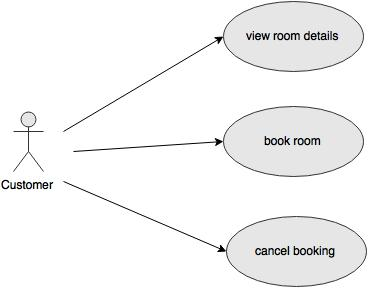
\includegraphics[width=0.8\textwidth]{figures/use-case-two}
\caption{Initial Use Case Model for Online Room Booking Application}
\label{fig:selection_by_use_case/use_case_two}
\end{center}
\end{figure}
\\
\\
\textbf{\underline{Step 2:}}
\\
\\
For each initial use case, task trees are generated which are needed to accomplish the desired functionality of respective use cases.
\\
\begin{table}[H]
  \centering
  \begin{adjustbox}{max width=\textwidth}
  \begin{tabular}{*{14}{|c}|}%%{|c|l|}
  \hline
  \textbf{Use Case} & \textbf{Task Tree} \\
  \hline
  book room & 
                 \begin{tabular}{ll}
                    \multirow{9}{*}
                    & customer enters access credentials\\
                    & system validates the credentials\\
                    & customer enters location and time details for booking\\
                    & system fetch the details of empty rooms according to the data provided\\
                    & system displays the details in muliple pages\\
                    & customer choose the room and submits for booking\\
                    & system generates a booking number\\
                    & System updates the room\\
                    & system sends notification to the customer regarding booking\\
                    \end{tabular}\\
                    \hline
   cancel booking   &
                    \begin{tabular}{ll}
                    \multirow{7}{*}
                    & customer enters access credentials\\
                    & system validates the credentials\\
                    & customer enters the booking number\\
                    & system validates the booking number\\
                    & customer cancels the booking\\
                    & system updates the room\\
                    & system sends notification to the customer regarding cancelation\\
                    \end{tabular}\\
                    \hline
   view room details &
                    \begin{tabular}{ll}
                    \multirow{5}{*}
                    & customer enters access credentials\\
                    & system validate the credentials\\
                    & customer enter location and time\\
                    & system fetch the details of empty rooms according to the data provided\\
                    & system display the details in multiple pages\\
                    \end{tabular}\\
                    \hline
\end{tabular}
\end{adjustbox}
  \caption{Task Trees for Initial Use Cases}
  \label{tab:selection_by_use_case/guidelines_for_use_case_refactoring/initial_task_tree}
\end{table}
\\
\textbf{\underline{Step 3:}}
\\
The initial task trees created for each use case at Step 2 is analysed. There are quite a few set of tasks which are functionally independent of the use case goal and also few tasks which are common in more use use cases. The following table \ref{tab:selection_by_use_case/guidelines_for_use_case_refactoring/common_and_independent_tasks} lists those tasks from the tasks trees \ref{tab:selection_by_use_case/guidelines_for_use_case_refactoring/initial_task_tree} which are either functionally independent from their corresponding use cases or common in more use cases.
\\
\begin{table}[H]
  \centering
  \begin{adjustbox}{max width=\textwidth}
  \begin{tabular}{*{14}{|c}|}%%{|c|l|}
  \hline
  \textbf{Tasks Type} & \textbf{Tasks} \\
  \hline
  Independent Tasks & 
                 \begin{tabular}{ll}
                    \multirow{9}{*}
                    & system validates the credentials\\
                    & system fetch the details of empty rooms according to the data provided\\
                    & system generates a booking number\\
                    & system validates the booking number\\
                    & system updates the room\\
                    & system sends notification to the customer
                    \end{tabular}\\
                    \hline
   Common Tasks   &
                \begin{tabular}{ll}
                    \multirow{9}{*}
                    & system validates the credentials\\
                    & system fetch the details of empty rooms according to the data provided\\
                    & system updates the room\\
                    & system sends notification to the customer
                    \end{tabular}\\
                    \hline
\end{tabular}
\end{adjustbox}
  \caption{Common and Independent Tasks}
  \label{tab:selection_by_use_case/guidelines_for_use_case_refactoring/common_and_independent_tasks}
\end{table}
\\
Now, for independent tasks the docomposition rule given by \ref{tab:selection_by_use_case/guidelines_for_use_case_refactoring/decomposition_rule} can be applied and for common tasks, the generalization rule given by \ref{tab:selection_by_use_case/guidelines_for_use_case_refactoring/generalization_rule} can be applied. The use cases obtained after applying these rules is shown by the figure \ref{fig:selection_by_use_case/use_case_three}
\\
\begin{figure}[H]
\begin{center}
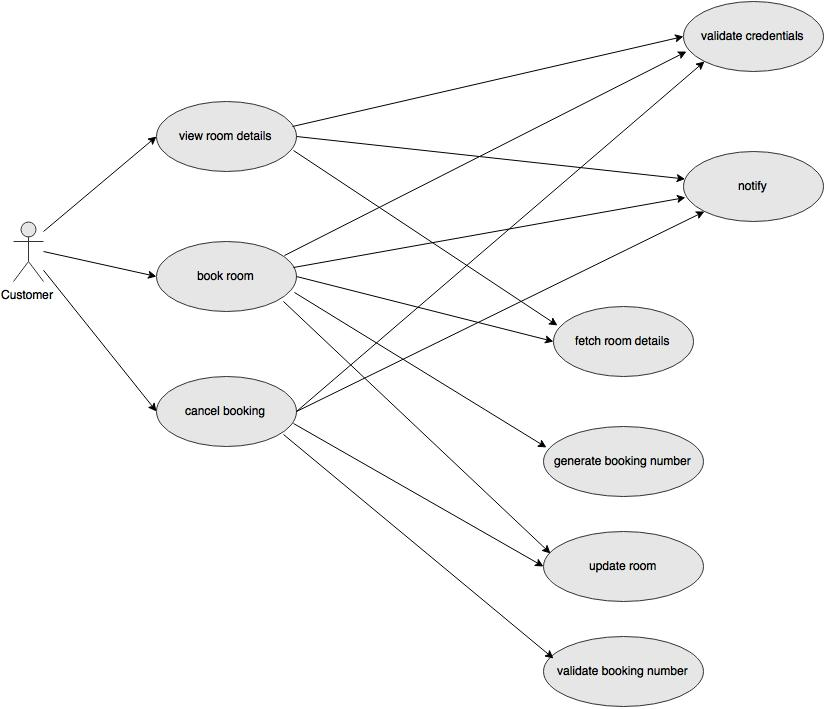
\includegraphics[width=0.8\textwidth]{figures/use-case-three}
\caption{Use Case Model after applying Decomposition and Generalization rules}
\label{fig:selection_by_use_case/use_case_three}
\end{center}
\end{figure}
\\
\textbf{\underline{Step 4:}}
\\
The use case model \ref{fig:selection_by_use_case/use_case_three} obtained in Step 3 is analysed again for further refactoring. It can seen that the use cases 'fetch room details' and 'update room' are fine grained and related to same business model 'Room'. Similarly, the use cases 'generate booking number' and 'validate booking number' are related to business entity 'Booking Number'. The composition rule given by \ref{tab:selection_by_use_case/guidelines_for_use_case_refactoring/composition_rule} can be applied to these use cases, which will then result in use case model given by figure \ref{fig:selection_by_use_case/use_case_four}
\\
\begin{figure}[H]
\begin{center}
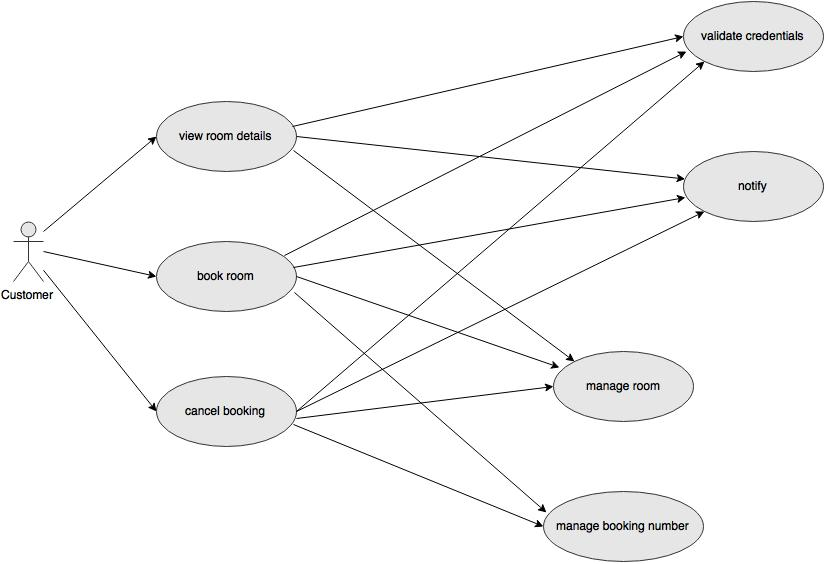
\includegraphics[width=0.8\textwidth]{figures/use-case-four}
\caption{Use Case Model after applying Composition rule}
\label{fig:selection_by_use_case/use_case_four}
\end{center}
\end{figure}
\\
\textbf{\underline{Step 5:}}
\\
Finally, the use case obtained in step 4 is used to identify the service candidates. The final use cases obtained in Step 4 have appropriate level of granularity and cohesive functionalities to be identified as individual services. Most importantly, the refactoring has now separated the cross cutting concerns in terms of various reusable fine grained use cases as shown by the figure. If we compare the the final use case model \ref{fig:selection_by_use_case/use_case_five} with respect to figure \ref{fig:selection_by_use_case/use_case_one}, then it can be implied that the functionalities operating on business entities as well as the business logic serving the candidate concerns are separated and represented by individual use cases. So, the each use case can be mapped to individual services. The services are as listed in the bottom of the figure \ref{fig:selection_by_use_case/use_case_five}.
\\
\begin{figure}[H]
\begin{center}
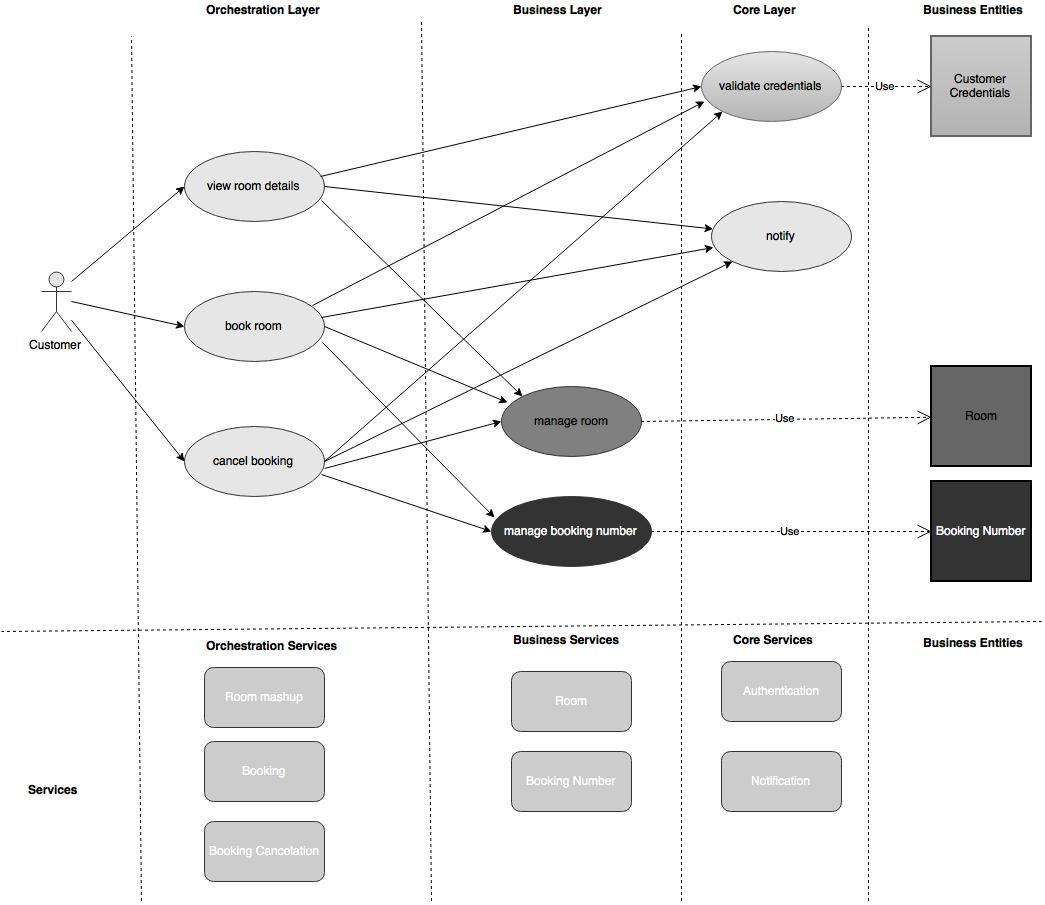
\includegraphics[width=0.8\textwidth]{figures/use-case-five}
\caption{Use Case Model for identification of service candidates}
\label{fig:selection_by_use_case/use_case_five}
\end{center}
\end{figure}
\\
\textbf{Service Layers}\\
The services or use cases obtained from the refactoring creates various levels of abstractions. The levels of abstractions represents different level of functionality. The services at the bottom layer are core services which serve many higher level services. These services are not dependent on any other services. 'Notification' and 'Authentication' are core services obtained from refactoring. The layer above the core layer is business layer. The business service can either have entity services, which control some related business entities or can have task services which provides some specific business logic to higher level services. 'Room' and 'Booking Number' are the entity services obtained from refactoring. Finally, the top layer is mashup layer which contains high level business logic and collaborates with business services as well as core services. 'Room mashup' , 'Booking' and 'Booking Cancelation' are orchestration layer services obtained. The individual services as well as their respective layers are given in figure \ref{fig:selection_by_use_case/use_case_five}. \cite{Fareghzadeh:2008aa}\cite{Emig:2015aa}\cite{Zimmermann:2005aa}

\chapter{Domain Driven Design}\label{chapter:domain_driven_design}

\section{Introduction}\label{section:domain_driven_design/introduction}
Understanding the problem space can be a very useful way to design software. The common way to understand the problem and communicate them is by using various design models. The design models are the abstraction as well as representation of the problem space. However, when the abstractions are created, there are chances that important concepts or data are ignored or misread. This will highly impact the quality of software produced. The software thus developed may not reflect the real world situation or problem entirely.
\\
Domain Driven Design provides a way to represent the real world problem space so that all the important concepts and data from real world remains intact in the model. The domain model thus captured respects the differences as well as the agreement in the concepts across various parts of the problem space. Moreover, it also provides a way to divide the problem space into manageable independent partitions and makes it easy for developers as well as stakeholders to focus on the area of concern as well as be more agile. Finally, the domain models act as the understandable and common view of the business for both domain experts as well as the developers. This will make sure that the software developed using domain driven design will comply with business need.\cite{Evans:2003aa}\cite{Vernon:2013aa}
\\

\section{Process to Domain Driven Design}\label{section:domain_driven_design/process_to_domain_driven_design}
There are three basic parts to implement domain driven design:
\begin{enumerate}
\item{Ubiquitous Language}
\item{Strategical Design}
\item{Tactical Design}
\end{enumerate}
\\
As the focus is to describe the process of identifying microservice candidates, only the first two parts are relevant and will be focused in the later part of this chapter.
\subsection{Ubiquitous Language}\label{section:domain_driven_design/process_to_domain_driven_design/ubiquitous_language}
Ubiquitous Language is a common language agreed among domain experts and developers in a team. It is important to have a common understanding about the concepts of a business which is being developed and ubiquitous language is the way to assure that. Domain Experts understand the domain in terms of their own jargon and concept. It is difficult for a developer to understand them. Usually, developers translates those jargons into the terms they understand easily during desing and implementation. However along the way of translation, major domain concepts can get lost and the immediate value of the resulting solution might decrease tremendously. In order to prevent creation of such low valued solution, there should be a meet-in-the-middle approach to define common vocabularies and concepts understood by all domain experts as well as the developers. These common vocabularies and concepts make the core of the ubiquitous language.\cite{Evans:2003aa}\cite{Vernon:2013aa}
\\
Along with the common vocabulary and concepts, domain models provide backbone to create ubiquitous language. The models represents not only artifacts but also functionalities, rules and strategies. It is a way to express the common understanding in a visual form providing an easy tool to comprehend.\cite{Evans:2003aa}\cite{Fowler:2006aa} According to \cite{Fowler:2003aa}, domain model should not be confused with data model which represents the business in datacentric view but rather each domain object should contain data as well as logic closely related to the data contained. Domain models are conceptual models rather than software artifacts but can be effectively visualized using \acrshort{UML}.\cite{Scott:2001aa}

\begin{figure}[H]
\begin{center}
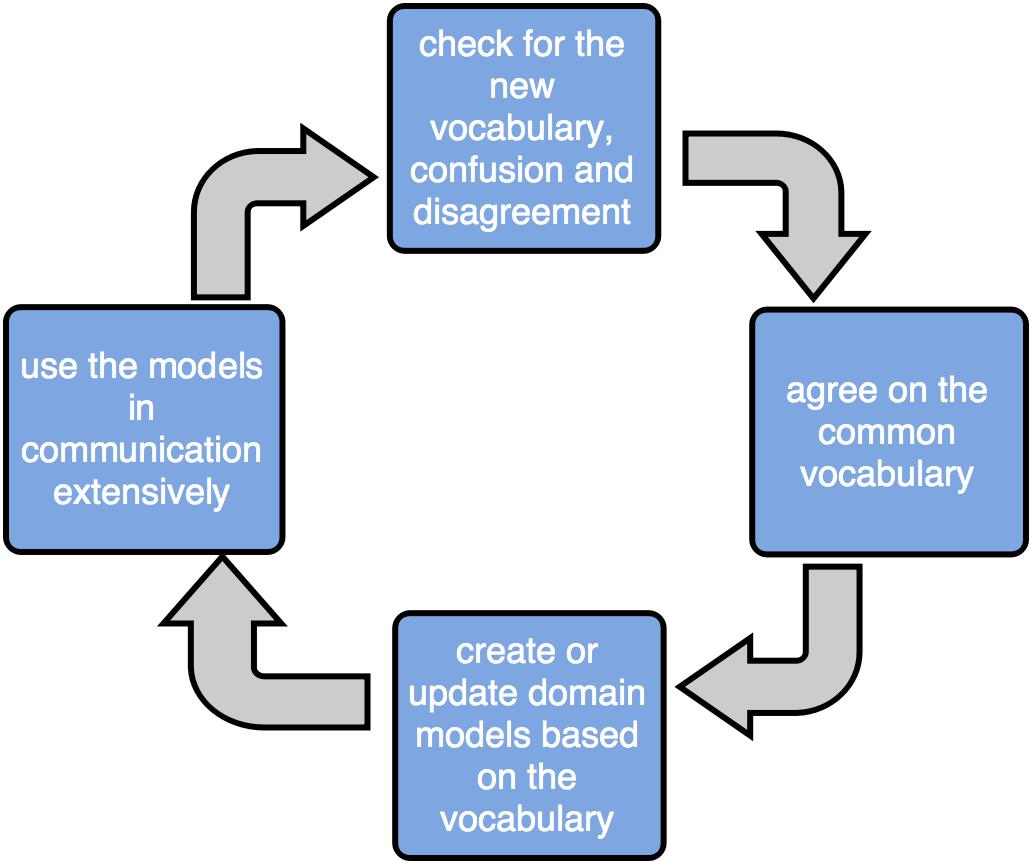
\includegraphics[width=0.8\textwidth]{figures/domain-driven-design-one}
\caption{Process to define Ubiquitous Language \cite{Evans:2003aa}}
\label{fig:domain_driven_design/ubiquitous_language_process}
\end{center}
\end{figure}
\\
The figure \ref{fig:domain_driven_design/ubiquitous_language_process} visualizes the process of discovering the ubiquitous language in any domain. It is not a discretely timed phenomenon but a continous procedure with various phases occuring in a cycle throughout the development.
\\
On arrival of any new term, concept or any confusion, the contextual meaning of those terms are made clear before adding to the domain vocabulary. Next, the vocabularies and concepts are used to create various domain models following \acrshort{UML}. The domain models and various vocabularies for the common laguage among domain experts and developers within the team. It is very important to use only domain vocabularies for communication and understanding which will not only help to reflect the hidden domain concepts in the implementation but also create opportunities to create new vocabularies or refine existing ones in the event of confusion and disagreement.\cite{Evans:2003aa}
\\
Thus, the common vocabulary and domain models form the core of the ubiquitous language and the only way of coming up with the better one is by applying it in communication extensively. Ubiquitous language is not just a collection or documentation of terms but is the approach of communication within a domain.
\\
\subsection{Strategical Design}\label{section:domain_driven_design/process_to_domain_driven_design/strategical_design}
When applying model-driven approach to an entire enterprise, the domain models get too large and complicated. It becomes difficult to analyse and understand all at once. Furthermore, it gets worse as the system gets bigger. The strategical design provides a way to divide the entire domain models into small,manageable and interoperable parts which can work together with low dependency in order to reflect the functionalities of the entire domain. The goal is to divide the system into modular parts which can be easily integrated. Additionally, the all-cohesive unified domain models of the entire enterprise cannot reflect differences in contextual vocabularies and concepts.\cite{Fowler:2014ab}\cite{Evans:2003aa}\cite{Vernon:2013aa}
\\
The strategical design specifies two major steps which are crucial in identifying microservices.
\\
\begin{shaded}Step 1: Divide problem domain into subdomains \end{shaded} \label{section:domain_driven_design/process_to_domain_driven_design/strategical_design/step_1}
\\
The domain represents the problem being solved by the software. The domain can be divided into various sub-domains based on the organizational structure of the enterprise, each sub-domain responsible for certain area of the problem. The \cite{Engels:2015aa} provides a comprehensive set of steps to identify sub-domains.
\begin{enumerate}
\item \textbf{Identify core business functionalities and map them into domain:} \\
A core business functionality represents the direct business capability which holds high importance and should be provided by the enterprise in order for it to succeed. For example, for any general e-commerce enterprise, the core focus will on the high amount orders being received from the customers and maintain the inventory to fulfil the orders. So, for those kind of e-commerce enterprises, 'Order Management' and 'Inventory Management' will be the some of the core domains.
\\
\item \textbf{Identify generic and supporting subdomains:} \\
The business capabilities which are viable for the success of business but not represent the specialization of the enterprise falls into supporting subdomains. The supporting subdomain does not require the enterprise to excel in these areas. Additionally, if the functionalities are not specific to the business but in a way support the business functionalities, then these are covered by generic subdomains. For example: for an e-commerce enterprise, 'Payment Management' can be a supporting subdomain whereas 'Reporting' and 'Authentication' can be generic subdomains.\cite{Vernon:2013aa}
\\
\item \textbf{Divide existing subdomains having multiple independent strategies:}\\
The subdomains found from earlier steps are analyzed to check if there are mutually independent strategies to handle the same functionality. The subdomain can then be further divided into multiple subdomains along the dimension of strategies. For example: the 'Payment Managment' subdomain discovered in earlier step can have different way of handling online payment depending upon the provider such as bank or paypal etc. In that case 'Payment Management' can be further divided into 'Bank Payment Management' and 'Paypal Payment Management'.
\end{enumerate}
\\
\begin{shaded}Step 2: Indentify bounded contexts\end{shaded} \label{section:domain_driven_design/process_to_domain_driven_design/strategical_design/step_2}
\\
As stated earlier of this section, the attempt to use a single set of domain models for the entire enterprise adds complexity for understanding and analysis. There is another important reason supporting the issue which is called unification of the domain models. Unification represents internal consistency of the terms and concepts described by the domain models. It is not always possible to have consistent meaning of terms without any contradictory rules throughout the enterprise. The identification of the logically consistent and inconsistent domain model creates a boundary around domain model. This boundary will bind all the terms which share consistent logic from those which are different from them so that there is clear understanding of the concept inside the boundary without any confusion. The shared context inside the boundary is defined as the bounded context.
\\
\textbf{Definition 1:} \label{bounded_context_definition_1}
\\
" A Bounded Context delimits the applicability of a particular model so that team members hava a clear and shared understanding of what has to be consistent and how it relates to other contexts. A bounded context has specific functionality and explicitly defines boundary around team organization, code bases and database schemas."\cite{Evans:2003aa}
\\
\textbf{Definition 2:} \label{bounded_context_definition_2}
\\
" A Bounded Context is an explicit boundary within which a domain model exists. Inside the boundary all terms and phrases of the Ubiquitous Language have specific meaning, and the model reflects the Language with exactness." \cite{Vernon:2013aa}
\\
\textbf{Definition 3:} \label{bounded_context_definition_3}
" A Bounded Context is a specific responsibility enforced by explicit boundaries." \cite{Mike:2012aa}
\\
Thus, the idea of bounded context provide the applicability of the ubiquitous language inside its boundary performing a specific responsibility. Outside the bounded contexts, teams have different ubiquitous language with different terms, concepts, meanings and functionalities. Apart from identifying independent and specific responsibilities inside a subdomain in order to identify bounded contexts, there are some general rules which can be considered as well.
\begin{enumerate}
\item \textbf{Assign individual bounded context to the subdomains identified in Step 1}
\\
Each subdomains have distinct functionalities and complete set of independent domain models to accomplish the functionalities. Thus, one to one mapping of subdomain and bounded context is possible ideally whereas in real cases, it may not be always possible which can be tackled using the rules discussed in further steps. For example: Order Management and Inventory Management can be two distinct bounded context each with own consistent ubiquitous language. \cite{Fowler:2014ab}\cite{Gorodinski:2013aa}
\\
\item \textbf{Identify polysemes}
\\
Polysemes are the terms which have different meaning in separate contexts. If the example of the generic subdomain 'Authentication' is taken. It can have an model 'Account' however the same model can refer to multiple concept such as social account identified by e-mail or registered account identified by unique username. The handling of these two separate concepts is also different which clearly suggests two separate context for each within 'Authentication' subdomain. Additionally, there can be polysemes in two separate domains as well. For example: there is also 'Account' model to identify bank account in the subdomain 'Bank Payment Management'. The identification of polysemes is vital to create clear boundary around which the concept and handling of such polysemes are consistent. \cite{Fowler:2014ab}
\\
\item \textbf{Identify independent generic functionality supporting the subdomain}
\\
There can be a necessity of independent technical functionality required to accomplish the business functionality of the subdomain only. Since it is only required by the particular subdomain, the functionality cannot be nominated as a generic subdomain. In such a case, the independent technical functionality can be realized as a separate bounded context. For example, in the subdomain 'Inventory Management', the functionality of full-text search can be assigned a separate bounded context as it is independent.\cite{Gorodinski:2013aa}
\end{enumerate}
\\
\section{Microservices and Bounded Context}\label{section:domain_driven_design/microservices_and_bounded_context}
Analyzing various definitions of microservices provided in section \ref{section:context/microservices_architecture_style}, a list of important features with respect to specific category such as granularity or quality was compiled in the table \ref{tab:context/microservices_architecture_style/keywords_extracted_from_various_definitions_of_microservice}. In addition to the definitions of bounded context provided in section \ref{bounded_context_definition_1}, the following definition of Domain Driven Design can be helpful to find analogy between a microservice and a bounded context.
\begin{shaded}Definition: Domain Driven Design\end{shaded}
"Domain Driven Design is about explaining what your company does in isolated parts, in performing these specific parts and you can have a dedicated team to do this stuff, and you can have different tools for different teams." \cite{Riggins:2015aa}
\\
\\
Using table \ref{tab:context/microservices_architecture_style/keywords_extracted_from_various_definitions_of_microservice} and concepts extracted from various definitions of bounded context as well as Domain Driven Design provided, the table \ref{tab:domain_driven_design/microservices_and_bounded_context/Analogy_of_Microservice_and_Bounded_Context} is generated. 
\\
\begin{table}[h!]
  \centering
  \begin{adjustbox}{max width=\textwidth}
  \begin{tabular}{*{14}{|c}|}%%{|c|c|}
  \hline
  \# & Expected features of a microservice  & Fulfilled by Bounded Context\\
  \hline
  \hline
   1 & Loosely coupled, related functions           & \checkmark  \\ \hline
   2 & Developed and deployed independently       & \checkmark \\ \hline
   3 & Own database                                 & \checkmark \\ \hline
   4 & Different database technologies         & \checkmark  \\ \hline
   5 & Build around Business Capabilities  & \checkmark\\ \hline
   6 & Different Programming Languages & \checkmark \\ \hline
   \hline
   \end{tabular}
\end{adjustbox}
  \caption{Analogy of Microservice and Bounded Context}
  \label{tab:domain_driven_design/microservices_and_bounded_context/Analogy_of_Microservice_and_Bounded_Context}
\end{table}
\\
The table \ref{tab:domain_driven_design/microservices_and_bounded_context/Analogy_of_Microservice_and_Bounded_Context} lists various features expected by a microservices. Again, it shows that the tabulated features are fulfilled by a bounded context. It can be implied that a microservice is conceptually analogous to a bounded context. The section \ref{section:domain_driven_design/process_to_domain_driven_design} provided the detailed process to discover bounded contexts within a large domain, which ultimately also provides guidelines to determine microservices using domain driven design principles.
\\
Furthermore, there can be found enough evidence regarding the analogy as well as practical implementation of the concept. The table lists various articles which agree on the analogy and in most cases, have utilized the concepts to create microservices in real world.
\begin{table}[h!]
  \centering
  \begin{adjustbox}{max width=\textwidth}
  \begin{tabular}{*{14}{|c}|}%%{|c|c|}
  \hline
  \# & Articles  & Agreement on the Concept & Utilized Bounded Context to create Microservices\\
  \hline
  \hline
   1 & \cite{Mauro:2015aa}           & \checkmark & \checkmark  \\ \hline
   2 & \cite{Hughson:2014aa}       & \checkmark & \\ \hline
   3 & \cite{Fowler:2014aa}        & \checkmark & \\ \hline
   4 & \cite{Sokhan:2015aa}       & \checkmark  & \\ \hline
   5 & \cite{Daya:2015aa}   & \checkmark & \checkmark \\ \hline
   6 & \cite{Riggins:2015aa} & \checkmark & \\ \hline
   7 & \cite{Beard:2015aa} & \checkmark  & \checkmark \\ \hline
   8 & \cite{Krylovskiy:2015aa} & \checkmark  & \checkmark \\ \hline
   9 & \cite{Viennot:2015aa} & \checkmark  & \checkmark \\ \hline
   10 & \cite{Balalaie:2015aa} & \checkmark  & \checkmark \\ \hline
   \hline
   \end{tabular}
\end{adjustbox}
  \caption{Application of Bounded Context to create Microservices}
  \label{tab:domain_driven_design/microservices_and_bounded_context/Microservices_following_Bounded_Context}
\end{table}
\\

\section{Example Scenario}\label{section:domain_driven_design/example_scenario}
In this section, a case study will be discussed. The case study will be used to design the system using microservices architecture following the domain driven design given supported by the section \ref{section:domain_driven_design/process_to_domain_driven_design}.

\begin{shaded} Case Study \end{shaded} \label{section:domain_driven_design/example_scenario/case_study}
The case study is for the same hotel introduced in the section \ref{section:selection_by_use_case/refactoring_example}. The hotel 'XYZ' is thinking of upgrading its current system and adding new business usecases in order to tune its competitive edge in the market.\\
Previously, the hotel only supported booking of the rooms, payment by cash, cancelation of booking and finally viewing of the room details.\\
The hotel has planned to provide various package offerings to the either general customers or specific group of customers satisfying certain profile. Firstly, a hotel staff creates a package with name, description, valid time period, applicable type of room and location and discount associated with the package. Furthermore, the package will also contain certain constraints such as maximum number of offerings and maximum number of offerings per customer. The offering is represented by coupon and has unique identity. Once a package is created, the package has to be activated either by the hotel staff or by the activation time trigger. Only, the activated packages are visible to the customers. The customers can apply for the active packages. The customer profile is validated against the expected profile for the package and then a new coupon is sent to the customer.\\
The room booking workflow has no changes from the old system where a customer can view list of rooms with various information and send room booking request to the system. The system will then send confirmation with unique booking code to the customer.\\
Finally, the payment can be done by debit card or by paypal. During the payment, the customer can specify a valid coupon. The payment system will then redeem the coupon so that the respective discount represented by the coupon is deducted from the overal price.\\
Additionally, a detailed report is planned to be made available for customers showing various transactions with the hotel for the room bookings along with the information of the rooms till date. Similarly, hotel staff has various types of reports such as profit statement and room booking status.\\
The steps listed in \ref{section:domain_driven_design/process_to_domain_driven_design} can be used to design the system defined by the case study \ref{section:domain_driven_design/example_scenario/case_study}.
\textbf{\underline{Step 1:}}
\\
With reference to the steps shown by the figure \ref{fig:domain_driven_design/ubiquitous_language_process}, the first step would be to find out new domain vocabularies, understand the meaning, agree on them and use them as the common vocabularies. The table \ref{tab:domain_driven_design/example_scenario/domain_keywords} lists some important domain terms taken from the case study \ref{section:domain_driven_design/example_scenario/case_study} and clarifies the meaning for each. It is interesting to notice that the term 'Profile' has two different meaning depending upon the context of package and customer and it is a polyseme.
\begin{table}[H]
  \centering
  \begin{adjustbox}{max width=\textwidth}
  \begin{tabular}{*{14}{|c}|}%%{|c|l|}
  \hline
  \textbf{Domain Terms} & \textbf{Definition} \\
  \hline
  Package & a discount offering to certain group of customers\\ \hline
  Profile & the expected characteristics of customers to be elligible to apply a package\\ \hline
  Discount & the reduction value offered in the total price for hotel service\\ \hline
  Constraint & defines the limitation of creating coupons for any package\\ \hline
  Coupon & represents the authorized assignment of a valid package to a valid customer, which can be used later\\ \hline
  Customer Profile & the current characteristics of a customer\\ \hline
  Room Booking & assignment of a room to a customer for certain period\\ \hline
  Booking Code & a unique code representing the valid room booking\\ \hline
  Redeem Coupon & request to use the coupon whereby the associated discount value is deducted from the total price\\ \hline
  Price & the total amount for the hotel service\\ \hline
\end{tabular}
\end{adjustbox}
  \caption{Domain Keywords}
  \label{tab:domain_driven_design/example_scenario/domain_keywords}
\end{table}
\\

\textbf{\underline{Step 2:}}
\\
Next, the subdomains are identified following the step 1 \ref{section:domain_driven_design/process_to_domain_driven_design/strategical_design/step_1} of strategical design. The core domains, supporting domains and generic domains are identified and listed in the table.
\\
\\
\begin{table}[H]
  \centering
  \begin{adjustbox}{max width=\textwidth}
  \begin{tabular}{*{14}{|c}|}%%{|c|l|}
  \hline
  \textbf{Core Domains} & 
                    \begin{tabular}{ll}
                    \multirow{3}{*}
                    & 1 Package\\
                    & 2 Booking\\
                    & 3 Checkout\\
                    \end{tabular}\\
                    \hline
                    
   \textbf{Supporting Domains} &
                    \begin{tabular}{ll}
                    \multirow{3}{*}
                    &
                    \begin{tabular}{ll}
                    \multirow{2}{*}{1 Payment}
                    & 1.1 Paypal\\
                    & 1.2 CardPayment\\
                    \end{tabular}\\
                    & 
                    \begin{tabular}{ll}
                    \multirow{2}{*}{2 User Management}
                    & 2.1 Customer Management\\
                    & 2.2 Staff Management\\
                    \end{tabular}\\
                    & 3 Room\\
                    \end{tabular}\\
                    \hline
                    
    \textbf{Generic Domains} &
                    \begin{tabular}{ll}
                    \multirow{2}{*}
                    & 1 Reporting\\
                    & 2 Authentication\\
                    \end{tabular}\\
                    \hline
\end{tabular}
\end{adjustbox}
  \caption{Subdomains}
  \label{tab:domain_driven_design/example_scenario/subdomains}
\end{table}
\\

The supporting domain "User Management" has different stragegy for Customer and Staff so can be further divided into "Customer Management" and "Staff Management" subdomains. For the same reason, the "Payment" subdomain can also be further divided into "Paypal" and "CardPayment".
\\
\textbf{\underline{Step 3:}}
\\
The next action is to identify bounded context following the process described in step \ref{section:domain_driven_design/process_to_domain_driven_design/strategical_design/step_2}. The process is implemented in each subdomains. In order to accomplish this, domain models can be constructed for each subdomain. Along the process, the various ambguities in the domain models and clear understanding of the concept of the models can be clarified. This will highly help to achieve consistent ubiquitious language with the unification of domain models as well as shared vocabulary inside each subdomain. The boundary around the uniform and consistent domain represents the bounded contexts. Additionally, the rules given in the section \ref{section:domain_driven_design/process_to_domain_driven_design/strategical_design/step_2} can be applied when appropriate to identify bounded contexts.
The following section will provide the analysis of major subdomains to identify the bounded contexts within.\\
\begin{shaded} Customer Management \end{shaded}
\\
\begin{figure}[H]
\begin{center}
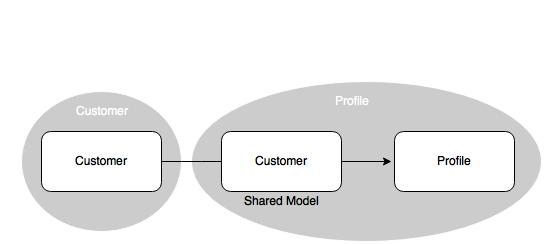
\includegraphics[width=0.8\textwidth]{figures/domain-driven-design-two}
\caption{Domain Model for Customer Management}
\label{fig:domain_driven_design/example_scenario/subdomains/Customer}
\end{center}
\end{figure}
\\
The management of customer includes two distinct broad task which are managing the customer itself and management of attributes of each customer which contribute to creating profile of customer at any point of time. Although, these two functionalities are related to customer, are actually loosely coupled and have different performance requirement. For eg: the change in the decision of adding attribute to a customer profile does not change the way customer is managed and also the rate at which customer profile is updated will definitely have high value than the rate customer is managed. Additionally, not all the attributes from customer is relevant to customer profile which makes 'Customer' a polyseme and a shared model between the two bounded contexts 'Customer' and 'Profile'.\\

\begin{shaded} Booking \end{shaded}
\\
\begin{figure}[H]
\begin{center}
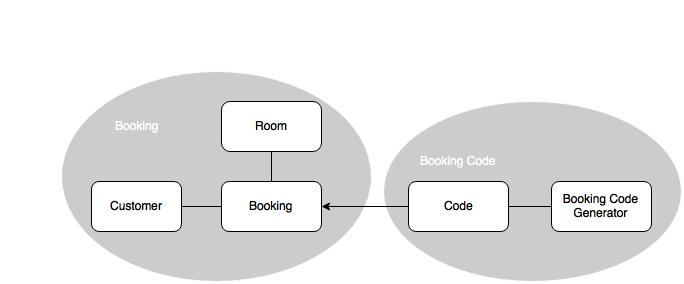
\includegraphics[width=0.8\textwidth]{figures/domain-driven-design-three}
\caption{Domain Model for Booking}
\label{fig:domain_driven_design/example_scenario/subdomains/booking}
\end{center}
\end{figure}
\\
The figure \ref{fig:domain_driven_design/example_scenario/subdomains/booking} shows the domain models of "Booking" subdomain. All the domain models and terms inside the subdomain are consistent and clear. However, the models 'Room', 'Customer', 'Booking' and 'Code' are closely related to booking functionality whereas the functionality of generating the booking code can be considered independent of booking. This gives two loosely coupled bounded contexts: "Booking" and "Booking Code". It is also interesting to notice that the models 'Customer' and 'Room' are polysemes with regard to other 'Customer' and 'Room' bounded contexts.\\
\begin{shaded} Checkout \end{shaded}
\\
\begin{figure}[H]
\begin{center}
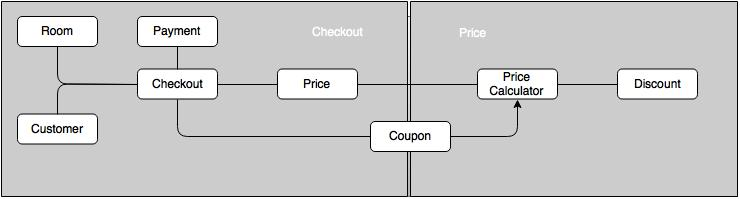
\includegraphics[width=0.8\textwidth]{figures/domain-driven-design-four}
\caption{Domain Model for Checkout}
\label{fig:domain_driven_design/example_scenario/subdomains/checkout}
\end{center}
\end{figure}
\\
The overall billing price calculation during checkout, which includes validation of coupon and redeem of the coupon onto the total price, is independent of the orchestration logic which occurs during checkout. The subdomain can be realized into two different bounded contexts 'Checkout' and 'Price'. Additionally, the domain models 'Customer, 'Discount', 'Room', 'coupon' and 'price' are polysemes for these bounded context with respect to other bounded contexts.\\
\begin{shaded} Package Management \end{shaded}
\\
\begin{figure}[H]
\begin{center}
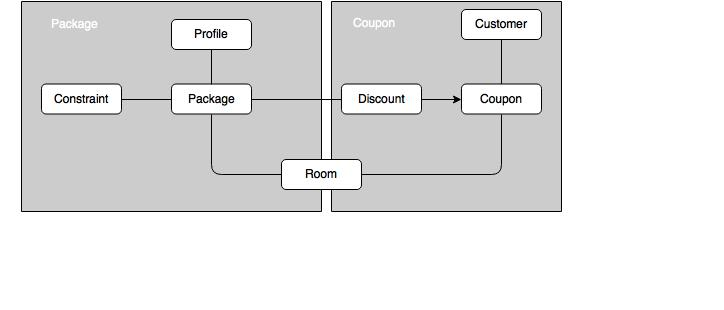
\includegraphics[width=0.8\textwidth]{figures/domain-driven-design-five}
\caption{Domain Model for Package Management}
\label{fig:domain_driven_design/example_scenario/subdomains/package-management}
\end{center}
\end{figure}
\\
The logic of package management can be considered independent of the way coupon is generated and validated. The packages are created by staff memeber whereas a coupon is created upon receiving a request from customer. Additionally, these are very specific and independent responsibilities, eligible of having own bounded contexts. The only data shared by the bounded contexts are about the information regarding eligible rooms and discount values. It should be made clear at this point that the 'Profile' domain model here is very different than 'Profile' domain model from 'Profile' boundend context of 'Customer Management' subdomain. In here, 'Profile' model defines the attributes of generic customer eligible for a specific package, however the 'Profile' domain model in 'Profile' bounded context provides the updated characteristics of any individual customer at the moment. Similarly, the models such as 'Customer' and 'Room' are polysemes.\\
The same process can be applied to identify bounded contexts for rest of the subdomains.
\chapter{Architecture at Hybris}\label{chapter:hybris_architecture}
\section{Overview}\label{section:hybris_architecture/overview}
SAP \acrshort{YaaS} provides a variety of business services to support as well as enhance the products offered as SAP hybris front office such as hybris Commerce, hybris Marketing, hybris Billing etc. Using these offered services, developers can create their own business services focussed on their customer requirements.\\
The figure \ref{fig:hybris_architecture/overview/yaas_overview} provides the overview of \acrshort{YaaS}. \acrshort{YaaS} provides various business processes as a service (bPaaS) essential to develop applications and services thus filling up the gap between SaaS and HCP. For that purpose, it consumes the application services (aPaaS) provided by \acrshort{HCP}.
\begin{figure}[H]
\begin{center}
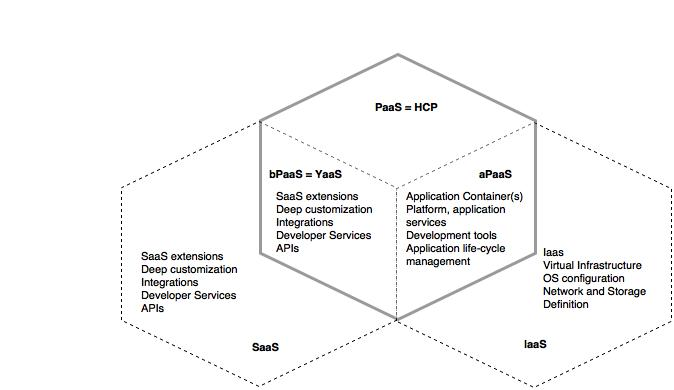
\includegraphics[width=0.8\textwidth]{figures/hybris-architecture-one}
\caption{\acrshort{YaaS} and \acrshort{HCP} \cite{Hirsch:2015aa}}
\label{fig:hybris_architecture/overview/yaas_overview}
\end{center}
\end{figure}
\\
\section{Vision}\label{section:hybris_architecture/vision}
The vision of \acrshort{YaaS} can be clarified with the following statement.
\begin{shaded}
"A cloud platform that allows everyone to easily develop, extend and sell services and applications." \\
\cite{Stubbe:2015aa}
\end{shaded}
The vision can be broadly categorized into following objectives.\\
\begin{enumerate}
\item \textbf{Cloud First}\\
The different parts of the application need to be scaled independently.
\item \textbf{Autonomy}\\
The development teams should be able to develop their modules independent of other teams and able to freely choose the technology that fits the job.
\item \textbf{Retain Speed}\\
The new features will be of value to customers if could be able to be released as fast as possible.
\item \textbf{Community}\\
It should be possible for the components to be shared across internal and external developers.
\end{enumerate}
The definition of microservices \ref{tab:context/microservices_architecture_style/keywords_extracted_from_various_definitions_of_microservice} as well as the characteristics of microservices [ref] signifies clearly that microservices architecture can be a good fit for \acrshort{YaaS} architecture.
\section{YaaS Architecture Principles}\label{section:hybris_architecture/YaaS_architecture_principles}
The Agile Manifesto \cite{Beck:2011aa} provides various principles to develop a software in a better way. It focus on fast response to the requirement changes with frequent continous delivery of software artifacts with close collaboration of customer and self-organizing teams.\\
The Reactive Manifesto \cite{Boner:2014aa} lists various qualities of a reactive system which includes responsiveness (acceptable consistent response time, quick detection and solution of problem), resilience (responsive during the event of failure) , elasticity (responsive during varying amount of workload) and asynchronous message passing. Loose coupling is highly focused.\\
Furthermore, the twelve factors from Heroku \cite{Wiggins:2012aa} provides a methodology for minimizing time and cost to develop software applications as services. It emphasizes on scalability of applications, explicit declaration as well as isolation of dependencies among components, multiple continuous deployments from a single version controlled codebase with separate pipelines for build, release and run.\\
Finally, the microservices architecture provides techiques of developing an application as a collection of autonomous small sized services focused on single responsibility. [section \ref{section:context/microservices_architecture_style}] It focus on independent deployment capability of individual microservices and suggest to use lightweight mechanisms such as http for communication among services. The architecture offers various advantages, few of them being individual independent scalability of each microservice, resilience achieved by isolating failure in a component and technology heterogeneity among various development teams.\cite{Newman:2015aa}
\\
Following the principles mentioned above, a list of principles are compiled to be used as guidelines for creating microservices. \cite{Stubbe:2015aa} The list of principles are listed below.
\textbf{\underline{the y-Factors}}
\\
\begin{enumerate}
\item \textbf{Self-Sufficient Teams}\\
The teams have independence and freedom for any decision related to the design and development of their components. This freedom is balanced by the responsibility for the team to handle the complete lifecycle of their components including smooth running as well as performance in production and troubleshooting in case of any problems.
\item \textbf{Open Technology landscape}\\
The team have freedom to choose any technology that they believe fits the requirement. They are completely responsible for the quality of their product. This gives teams, ownership as well as satisfaction for their products.
\item \textbf{Release early, release often}\\
The agile manifesto and twelve factors from Heroku also focus on continuous delivery of product to the clients. This will decrease time of feedback and ultimately fast response to the feedback resulting in high customer satisfaction. The teams are responsible to create build and delivery pipeline for all available environments.
\item \textbf{Responsibility}\\
The teams are the only responsible groups to work directly with the customers on behalf of their products. They need to work on the feedback provided by the customers. It will increase the quality of the products and relationship with customers. All the responsibilities including scaling, maintaining, supporting and improving products are handled by respective teams.
\item \textbf{\acrshort{API}s first}\\
The \acrshort{API} is a contract between service and consumers. The decision regarding design and development is very important as it can be one of the greatest assets if good or else can be a huge liability if done bad. \cite{Bloch:2016aa} The articles \cite{Bloch:2016aa} and \cite{Blanchette:2008aa} list various characteristics of good \acrshort{API} including simplicity, extensibility, maintainability, completeness, small and focussing on single functionality. Furthermore, a good approach to develop \acrshort{API} is to first design iteratively before implementation in order to understand the requirement clearly. Another important aspect of a good \acrshort{API} among many is complete and updated documentation.
\item \textbf{Predictable and easy-to-use UI}\\
The user interfaces should be simple, consistent across the system and also consistent to various user friendly patterns.\cite{Sollenberger:2012aa} The articles \cite{Martin:2013aa} and \cite{Porter:2016aa} specify additional principles to be considered when designing user interfaces. A few of them includes providing clarity with regard to purpose, smart organization and respecting the expectation as well as requirements of customers.
\item \textbf{Small and Simple Services}
A service should be small and focused on cohesive functionalities. The concept closely relates to the single responsibility principle. \cite{Martin:2016aa} A good approach is to explicitly create boundaries around business capabilities.\cite{Newman:2015aa}
\item \textbf{Scalability of technology}\\
The choice of technologies should be cloud friendly such that the products can scale cost-efficiently and without delay. It is influenced by the elasticity principle provided by the reactive manifesto.\cite{Boner:2014aa}
\item \textbf{Design for failure}
The service should be responsive in the time of failure. It can be possible by containment and isolation of failure within each component. Similarly, the recovery should be handled gracefully without affecting the overal availability of the entire system. \cite{Boner:2014aa}
\item \textbf{Independent Services}\\
The services should be autonomous. Each service should be able to be deployed independently. The services should be loosely coupled, they could be changed independently of eachother. The concept is highly enforced by exposing functionalities via \acrshort{API}s and using lightweight network calls as only way of communication among services. \cite{Newman:2015aa}
\item \textbf{Understand Your System}
It is crucial to have a good understanding of problem domain in order to create a good design. The concept of domain driven design strongly motivates this approach to indentify individual autonomous components, their boundaries and the communication patterns among them. \cite{Newman:2015aa} Furthermore, it is also important to understand the expectations of consumers regarding performance and then to realize them accordingly. It is possible only by installing necessary operational capabilities such as continuous delivery, monitoring, scaling and resilience.
\end{enumerate}
 \section{Interviews}\label{section:hybris_architecture/interview}
 With the intension to anticipate the overall belief, culture and practice followed by hybris to develop \acrshort{YaaS}, a number of interviews were conducted with a subset of key personnels who are directly involved in \acrshort{YaaS}. The list of interviewees with their corresponsing roles is shown in the table \ref{tab:hybris_architecture/interview/interviewee_list}. In order to preserve anonymity, the real names are replaced with forged ones.
\begin{table}[H]
  \centering
  \begin{adjustbox}{max width=\textwidth}
  \begin{tabular}{*{14}{|c}|}%%{|c|l|}
  \hline
\textbf{Names}          & \textbf{Roles}\\      \hline
John Doe                & Product Manager\\     \hline
Ivan Horvat             & Senior Developer\\    \hline
Jane Doe                & Product Manager\\     \hline
Mario Rossi             & Product Manager\\     \hline
Nanashi No Gombe        & Product Manager\\     \hline
Hans Meier              & Architect\\           \hline
Otto Normalverbraucher  & Product Manager\\     \hline
Jan Kowalski            & Senior Developer\\    \hline
\end{tabular}
\end{adjustbox}
  \caption{Interviewee List}
  \label{tab:hybris_architecture/interview/interviewee_list}
\end{table}
\\
\subsection{Hypothesis}\label{section:hybris_architecture/interview/hypothesis}
During the process of solving the concerned research questions, various topics of high value have been discovered. The topics are:\\
\begin{enumerate}
\item Granularity
\item Quality Attributes
\item Process to design microservices
\end{enumerate}
\\
Similarly, based on research findings, a list of hypothesis has been made with respect to each topic.

\begin{shaded}
Hypothesis 1:
\end{shaded}\label{section:hybris_architecture/interview/hypothesis_1}
\textbf{The correct size of microservices is determined by: \begin{enumerate}\item Single Responsibility Principle \item Autonomy, and \item Infrastructure Capability \end{enumerate}}
\\
According S.Newman, a good microservices should be small and focus on accomplishing one thing well. Additionally, it could be independently deployed and updated. This strongly suggests the requirement of autonomy. \cite{Newman:2015aa} Futhermore, M. Stine also agree that the size of a microservices should be determined by single responsibility principle. \cite{Stine:2014aa}
Also, the principle listed in \ref{principle:granularity/IT_infrastructure} indicate that the advancement in the current technology and culture of the organization also defines size of microservices. \cite{Pierre-Reldin:2007aa}
\begin{shaded}
Hypothesis 2:
\end{shaded} \label{section:hybris_architecture/interview/hypothesis_2}
\textbf{Domain driven design is the optimum approach to design microservices.}
\\
\\
The concept of domain driven design to design microservices is promoted by S. Newman and M. Fowler. \cite{Newman:2015aa} \cite{Fowler:2014aa} Similary, there can be found evendence of domain driven design being used in various projects to design microservices. The list of projects is shown in the table \ref{tab:domain_driven_design/microservices_and_bounded_context/Microservices_following_Bounded_Context}.
\\
\subsection{Interview Compilation}\label{section:hybris_architecture/interview/interview_compilation}
For each topic listed above in section \ref{section:hybris_architecture/interview/hypothesis}, a list of questionaires is prepared. The questions were then asked to the interviewees. In the remaining part of this section, an attempt is made to compile the response from the interviews on the questionaires for each topic.
\\
\textbf{\underline{1. Granularity}}\\  
\begin{shaded} Question 1.1 \end{shaded} \label{question:hybris_architecture/interview/question_1.1}
"Do you consider the size of microservices when desigining microservice architecture?"\\
\begin{table}[H]
\centering
\begin{adjustbox}{max width=\textwidth}
\begin{tabular}{*{14}{|c}|}%%{|c|l|l|l|l|l|l|l|l|l|}
\hline
\textbf{Response 1.1} & John & Ivan & Jane & Mario & Nanashi & Hans & Otto & Jan & \textbf{Score}\\
 \hline
Important               & 1 & 1 & 1 & 0 & 1 & 1 & 0 & 0 & \textbf{5}    \\ 
 \hline
Secondary, Not primary  & 0 & 0 & 0 & 1 & 0 & 0 & 1 & 1 & \textbf{3} \\ 
 \hline
Not Important           & 0 & 0 & 0 & 0 & 0 & 0 & 0 & 0 & \textbf{0} \\ 
 \hline
 \hline
\end{tabular}
\end{adjustbox}
\label{tab:hybris_architecture/interview/question_1.1}
\end{table}
\\
\\
\begin{comment}
\begin{figure}[H]
\begin{center}
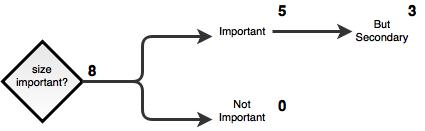
\includegraphics[width=0.9\textwidth]{figures/hybris_architecture_question_1_1}
\label{fig:hybris_architecture/interview/hybris-architecture-question-1-1}
\end{center}
\end{figure}
\\
\end{comment}

\\
\begin{figure}[H]
\begin{center}
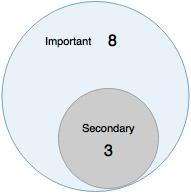
\includegraphics[scale=0.5]{figures/question1_1}
\label{fig:hybris_architecture/interview/question1-1}
\end{center}
\end{figure}
\\

\begin{shaded} Question 1.2 \end{shaded} \label{question:hybris_architecture/interview/question_1.2}
"How do you measure size of a microservice?"\\
\begin{table}[H]
\centering
\begin{adjustbox}{max width=\textwidth}
\begin{tabular}{*{14}{|c}|}%%{|c|c|l|l|l|l|l|l|l|l|l|}
\hline
\multicolumn{2}{|c|}{\textbf{Response 1.2} }& John & Ivan & Jane & Mario & Nanashi & Hans & Otto & Jan & \textbf{Score}\\
 \hline
 \hline
\multicolumn{2}{|c|}{\textit{Qualitatively}}               & 1 & 1 & 1 & 1 & 1 & 1 & 1 & 1 & \textbf{8}    \\ 
 \hline
a.& Functionality  & 1 & 1 & 1 & 1 & 1 & 1 & 1 & 1 & \textbf{8}\\ 
 \hline
b.& Business value           & 1 & 1 & 1 & 1 & 1 & 1 & 1 & 1 & \textbf{8} \\ 
 \hline
 \hline
 \multicolumn{2}{|c|}{\textit{Quantitatively}}               & 0 & 0 & 0 & 0 & 0 & 0 & 0 & 0 & \textbf{0}    \\ 
 \hline
 \hline
\end{tabular}
\end{adjustbox}
\label{tab:hybris_architecture/interview/question_1.2}
\end{table}
\\
\begin{comment}
\\
\begin{figure}[H]
\begin{center}
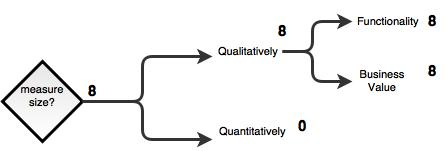
\includegraphics[width=0.9\textwidth]{figures/hybris_architecture_question_1_2}
\label{fig:hybris_architecture/interview/hybris-architecture-question-1-2}
\end{center}
\end{figure}
\\
\end{comment}

\\
\begin{figure}[H]
\begin{center}
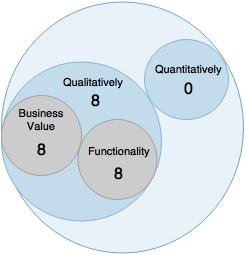
\includegraphics[scale=0.5]{figures/question1_2}
\label{fig:hybris_architecture/interview/question1-2}
\end{center}
\end{figure}
\\

\begin{shaded} Question 1.3 \end{shaded} \label{question:hybris_architecture/interview/question_1.3}
"What kind of size do you try to achieve for a microservice?"\\

\begin{table}[H]
\centering
\begin{adjustbox}{max width=\textwidth}
\begin{tabular}{*{14}{|c}|}%%{|c|c|l|l|l|l|l|l|l|l|l|}
\hline
\multicolumn{2}{|c|}{\textbf{Response 1.3} }
                                    & John & Ivan & Jane & Mario & Nanashi & Hans & Otto & Jan & \textbf{Score}\\
 \hline
 \hline
\multicolumn{2}{|c|}{\textit{as small as possible in terms of functionality}}               
                                    & 1 & 1 & 1 & 1 & 1 & 1 & 1 & 1 & \textbf{8}    \\ 
 \hline
 \hline
 \multicolumn{2}{|c|}{\textit{influenced by other attributes}}               
                                    &   &   &   &   &   &   &   &   &     \\ 
 \hline
a.& Business Value                  & 1 & 1 & 1 & 1 & 1 & 1 & 1 & 1 & \textbf{8}\\ 
 \hline
b.& Single Responsibility           & 1 & 1 & 1 & 1 & 1 & 1 & 1 & 1 & \textbf{8} \\ 
 \hline
c.& Loose Coupling                  & 0 & 1 & 0 & 0 & 1 & 1 & 0 & 1 & \textbf{4} \\ 
 \hline
d.& Cohesion                        & 0 & 1 & 0 & 0 & 0 & 0 & 1 & 1 & \textbf{3} \\ 
 \hline
e.& Autonomy                        & 0 & 1 & 1 & 0 & 0 & 1 & 0 & 0 & \textbf{3} \\ 
 \hline
f.& Maintainability                 & 0 & 1 & 0 & 0 & 0 & 1 & 1 & 0 & \textbf{3} \\ 
 \hline
g.& Reusability                     & 0 & 1 & 0 & 0 & 1 & 1 & 1 & 0 & \textbf{4} \\ 
 \hline
h.& Scalability                     & 1 & 1 & 0 & 1 & 1 & 1 & 1 & 0 & \textbf{6} \\ 
 \hline
i.& Network Complexity              & 1 & 0 & 0 & 0 & 1 & 1 & 0 & 0 & \textbf{3} \\ 
 \hline
 \hline
\end{tabular}
\end{adjustbox}
\label{tab:hybris_architecture/interview/question_1.3}
\end{table}
\\
\begin{comment}
\\
\begin{figure}[H]
\begin{center}
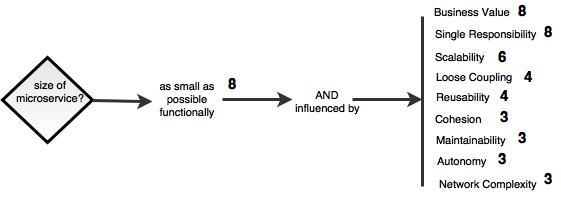
\includegraphics[width=0.9\textwidth]{figures/hybris_architecture_question_1_3}
\label{fig:hybris_architecture/interview/hybris-architecture-question-1-3}
\end{center}
\end{figure}
\\
\end{comment}
\\
\begin{figure}[H]
\begin{center}
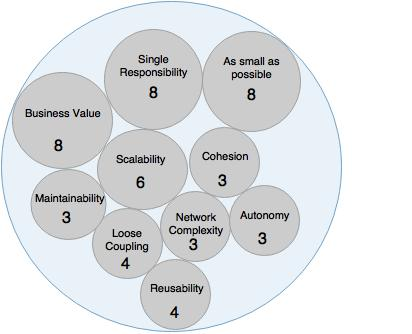
\includegraphics[scale=0.5]{figures/question1_3}
\label{fig:hybris_architecture/interview/question1-3}
\end{center}
\end{figure}
\\
\begin{shaded} Question 1.4 \end{shaded} \label{question:hybris_architecture/interview/question_1.4}
"Suppose that you do not have the agile culture like continuous integration and delivery automation and also cloud infrastructure. How will it affect your decision regarding microservices and their size?"\\
\begin{table}[H]
\centering
\begin{adjustbox}{max width=\textwidth}
\begin{tabular}{*{14}{|c}|}%%{|c|l|l|l|l|l|l|l|l|l|}
\hline
\textbf{Response 1.4}   & John & Ivan & Jane & Mario & Nanashi & Hans & Otto & Jan & \textbf{Score}\\
 \hline
 \begin{tabular}{ll}
                    \multirow{2}{*}
                    & No microservices at all, start with Monolith,\\
                    & extract one microservice at a time as automation matures\\
                    \end{tabular}
               
                                & 1 & 1 & 0 & 1 & 1 & 1 & 1 & 1 & \textbf{7}    \\ 
 \hline
  \begin{tabular}{ll}
                    \multirow{2}{*}
                    & Start with bigger sized microservices with\\
                    & high business value, low coupling and single Responsibility\\
                    \end{tabular}  
                                & 0 & 0 & 1 & 0 & 1 & 0 & 1 & 0 & \textbf{3} \\ 
 \hline
 \hline
\end{tabular}
\end{adjustbox}
\label{tab:hybris_architecture/interview/question_1.4}
\end{table}
\\
\begin{comment}
\\
\begin{figure}[H]
\begin{center}
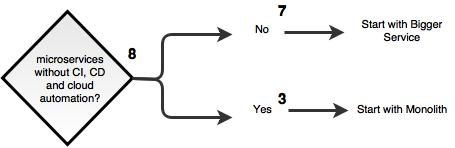
\includegraphics[width=0.9\textwidth]{figures/hybris_architecture_question_1_4}
\label{fig:hybris_architecture/interview/hybris-architecture-question-1-4}
\end{center}
\end{figure}
\\
\\
\begin{figure}[H]
\begin{center}
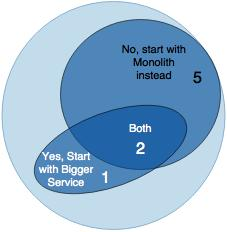
\includegraphics[scale=0.5]{figures/question1_4}
\label{fig:hybris_architecture/interview/question1-4}
\end{center}
\end{figure}
\\
\end{comment
}
\begin{shaded} Question 1.5 \end{shaded} \label{question:hybris_architecture/interview/question_1.5}
"Are you facing any complexities because of microservices architecture and the size you have chosen?"\\
\begin{table}[H]
\centering
\begin{adjustbox}{max width=\textwidth}
\begin{tabular}{*{14}{|c}|}%%{|c|l|l|l|l|l|l|l|l|l|}
\hline
\textbf{Response 1.5}   & John & Ivan & Jane & Mario & Nanashi & Hans & Otto & Jan & \textbf{Score}\\
 \hline
communication overhead in network               & 0 & 1 & 0 & 0 & 0 & 0 & 1 & 0 & \textbf{2}    \\ 
 \hline
complexity in failure handling  & 0 & 1 & 0 & 0 & 0 & 0 & 0 & 0 & \textbf{1} \\ 
 \hline
Monitoring is difficult           & 0 & 1 & 0 & 0 & 0 & 0 & 1 & 0 & \textbf{1} \\ 
 \hline
 Operational support is costly           & 0 & 1 & 1 & 0 & 0 & 0 & 0 & 0 & \textbf{2} \\ 
 \hline
 difficult to trace a request           & 0 & 1 & 1 & 0 & 0 & 0 & 0 & 0 & \textbf{2} \\ 
 \hline
 updates can be difficult due to dependencies among microservices          & 0 & 0 & 1 & 0 & 0 & 0 & 0 & 0 & \textbf{1} \\ 
 \hline
 \hline
\end{tabular}
\end{adjustbox}
\label{tab:hybris_architecture/interview/question_1.5}
\end{table}
\\


\textbf{\underline{2. Quality Attributes}}\\
\begin{shaded} Question 2.1 \end{shaded} \label{question:hybris_architecture/interview/question_2.1}
"Do you consider any quality attributes when selecting microservices?"\\
\begin{table}[H]
\centering
\begin{adjustbox}{max width=\textwidth}
\begin{tabular}{*{14}{|c}|}%%{|c|l|l|l|l|l|l|l|l|l|}
\hline
\textbf{Response 2.1}   & John & Ivan & Jane & Mario & Nanashi & Hans & Otto & Jan & \textbf{Score}\\
 \hline
Loose Coupling          & 1 & 1 & 1 & 1 & 1 & 1 & 1 & 1 & \textbf{8}    \\ 
 \hline
Cohesion                & 1 & 1 & 1 & 1 & 1 & 1 & 0 & 1 & \textbf{7}    \\ 
 \hline
 Autonomy               & 1 & 1 & 0 & 0 & 0 & 1 & 1 & 0 & \textbf{4}    \\ 
 \hline
 Scalability            & 1 & 0 & 0 & 1 & 1 & 0 & 1 & 1 & \textbf{5}    \\ 
 \hline
 Complexity             & 1 & 0 & 0 & 0 & 1 & 0 & 1 & 0 & \textbf{3}    \\ 
 \hline
 Reusability            & 0 & 1 & 0 & 0 & 0 & 0 & 1 & 0 & \textbf{2}    \\ 
 \hline
 \hline
\end{tabular}
\end{adjustbox}
\label{tab:hybris_architecture/interview/question_2.1}
\end{table}
\\

\begin{shaded} Question 2.2 \end{shaded} \label{question:hybris_architecture/interview/question_2.2}
"Do you consider any metrics for evaluating the quality attributes?"\\
\begin{table}[H]
\centering
\begin{adjustbox}{max width=\textwidth}
\begin{tabular}{*{14}{|c}|}%%{|c|l|l|l|l|l|l|l|l|l|}
\hline
\textbf{Response 2.2}   & John & Ivan & Jane & Mario & Nanashi & Hans & Otto & Jan & \textbf{Score}\\
 \hline
No          & 1 & 1 & 1 & 1 & 1 & 1 & 1 & 1 & \textbf{8}    \\ 
 \hline
Yes                & 0 & 0 & 0 & 0 & 0 & 0 & 0 & 0 & \textbf{0}    \\ 
 \hline
\end{tabular}
\end{adjustbox}
\label{tab:hybris_architecture/interview/question_2.2}
\end{table}
\\
\begin{comment}
\\
\begin{figure}[H]
\begin{center}
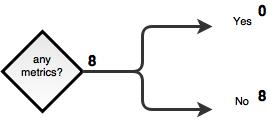
\includegraphics[scale=0.5]{figures/hybris_architecture_question_2_2}
\label{fig:hybris_architecture/interview/hybris-architecture-question-2-2}
\end{center}
\end{figure}
\\
\end{comment}
\\
\begin{figure}[H]
\begin{center}
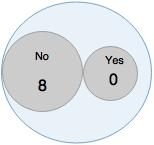
\includegraphics[scale=0.5]{figures/question2_2}
\label{fig:hybris_architecture/interview/question2-2}
\end{center}
\end{figure}
\\
\begin{shaded} Question 2.3 \end{shaded} \label{question:hybris_architecture/interview/question_2.3}
"Do you think the table of basic metrics can be helpful?"\\
\begin{table}[H]
\centering
\begin{adjustbox}{max width=\textwidth}
\begin{tabular}{*{14}{|c}|}%%{|c|l|l|l|l|l|l|l|l|l|}
\hline
\textbf{Response 2.3}   & John & Ivan & Jane & Mario & Nanashi & Hans & Otto & Jan & \textbf{Score}\\
 \hline
No          & 0 & 0 & 0 & 0 & 0 & 0 & 0 & 0 & \textbf{0}    \\ 
 \hline
Yes                & 1 & 0 & 1 & 0 & 1 & 0 & 1 & 0 & \textbf{4}    \\ 
 \hline
Maybe                & 0 & 1 & 0 & 1 & 0 & 1 & 0 & 1 & \textbf{4}    \\ 
 \hline
 \hline
\end{tabular}
\end{adjustbox}
\label{tab:hybris_architecture/interview/question_2.3}
\end{table}
\\
\begin{comment}
\\
\begin{figure}[H]
\begin{center}
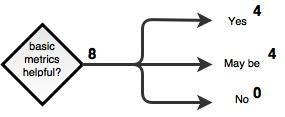
\includegraphics[scale=0.5]{figures/hybris_architecture_question_2_3}
\label{fig:hybris_architecture/interview/hybris-architecture-question-2-3}
\end{center}
\end{figure}
\\
\end{comment}
\\
\begin{figure}[H]
\begin{center}
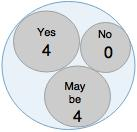
\includegraphics[scale=0.5]{figures/question2_3}
\label{fig:hybris_architecture/interview/question2-3}
\end{center}
\end{figure}
\\
\textbf{\underline{3. Process to design microservices}}\\
\begin{shaded} Question 3.1 \end{shaded} \label{question:hybris_architecture/interview/question_3.1}
"Do you follow specific set of consistent procedures across the teams to discover microservices?"\\
\begin{table}[H]
\centering
\begin{adjustbox}{max width=\textwidth}
\begin{tabular}{*{14}{|c}|}%%{|c|l|l|l|l|l|l|l|l|l|}
\hline
\textbf{Response 3.1}   & John & Ivan & Jane & Mario & Nanashi & Hans & Otto & Jan & \textbf{Score}\\
 \hline
No          & 1 & 1 & 1 & 1 & 1 & 1 & 1 & 1 & \textbf{8}    \\ 
 \hline
Yes                & 0 & 0 & 0 & 0 & 0 & 0 & 0 & 0 & \textbf{0}    \\ 
 \hline
\end{tabular}
\end{adjustbox}
\label{tab:hybris_architecture/interview/question_2.3}
\end{table}
\\
\begin{comment}
\\
\begin{figure}[H]
\begin{center}
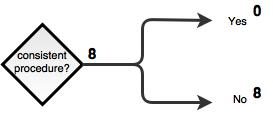
\includegraphics[scale=0.5]{figures/hybris_architecture_question_3_1}
\label{fig:hybris_architecture/interview/hybris-architecture-question-3-1}
\end{center}
\end{figure}
\\
\end{comment}
\\
\begin{figure}[H]
\begin{center}
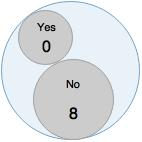
\includegraphics[scale=0.5]{figures/question3_1}
\label{fig:hybris_architecture/interview/question3-1}
\end{center}
\end{figure}
\\
\begin{shaded} Question 3.2 \end{shaded} \label{question:hybris_architecture/interview/question_3.2}
"Can you define the process you follow to come up with microservices?"\\
\begin{table}[H]
\centering
\begin{adjustbox}{max width=\textwidth}
\begin{tabular}{*{14}{|c}|}%%{|c|l|l|l|l|l|l|l|l|l|l|}
\hline
\multicolumn{3}{|c|}{\textbf{Response 3.2}}   & John & Ivan & Jane & Mario & Nanashi & Hans & Otto & Jan & \textbf{Score}\\
\hline
\hline
\multicolumn{3}{|c|}{
\begin{tabular}{ll}
\multirow{4}{*}
& By brain-storming to divide a usecase into finer\\
& functionalities considering business value, cohesion,\\
& loose coupling [Single Responsibility], autonomy,\\
& reusability and scalability.
\end{tabular}}
                                            & 1 & 0 & 1 & 1 & 0 & 0 & 1 & 1 & \textbf{5}    \\ 
 \hline
& \multicolumn{2}{|c|}{\textit{Have you heard of Domain driven design and bounded context?}}               
                                            &   &   &   &   &   &   &   &   &      \\ 
 \hline
 & & Yes                                    & 0 &   & 0 & 0 &   &   & 1 & 0 & \textbf{1}    \\ 
 \hline
 & \multicolumn{2}{|c|}{\textit{Is the concept provided by bounded context being used?}}               
                                            &   &   &   &   &   &   &   &   &      \\ 
 \hline
 & & Yes                                    & 1 & 0 & 1 & 0 & 0 & 0 & 1 & 0 & \textbf{3}    \\
 \hline
 \hline
\multicolumn{3}{|c|}{
\begin{tabular}{ll}
\multirow{4}{*}
& By identifying bounded context using domain-driven-design\\
& Understand the problem domain interacting with\\
& domain experts and studying the interaction among\\
& domain models and flow of data.
\end{tabular}}
                                            & 0 & 1 & 0 & 0 & 1 & 1 & 1 & 0 & \textbf{4}    \\ 
\hline
\hline
\end{tabular}
\end{adjustbox}
\label{tab:hybris_architecture/interview/question_3.2}
\end{table}
\\
\begin{comment}
\\
\begin{figure}[H]
\begin{center}
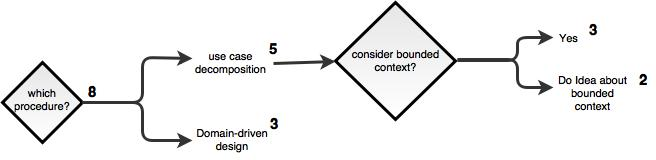
\includegraphics[scale=0.5]{figures/hybris_architecture_question_3_2}
\label{fig:hybris_architecture/interview/hybris-architecture-question-3-2}
\end{center}
\end{figure}
\\
\end{comment}
\\
\begin{figure}[H]
\begin{center}
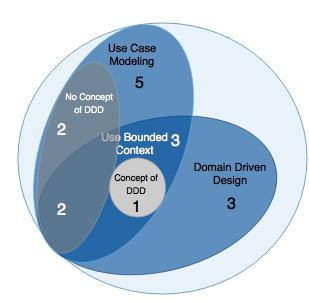
\includegraphics[scale=0.5]{figures/question3_2}
\label{fig:hybris_architecture/interview/question3-2}
\end{center}
\end{figure}
\\
\subsection{Interview Reflection on Hypothesis}\label{section:hybris_architecture/interview/interview_reflection_on_hypothesis}
The data gathered from the interviews which are compiled in the section \ref{section:hybris_architecture/interview/interview_compilation} can be a good source to analyse the hypothesis listed on the section \ref{section:hybris_architecture/interview/hypothesis}.
\\
\begin{shaded} Hypothesis 1 \end{shaded}
\textbf{The correct size of microservices is determined by: \begin{enumerate}\item Single Responsibility Principle \item Autonomy, and \item Infrastructure Capability \end{enumerate}}
\\
The response from question \ref{question:hybris_architecture/interview/question_1.3} has helped to point out some important constraints which play significant role in industry while choosing appropriate size of microservice. It is also interesting to notice how the terms in answer closely relate to the hypothesis \ref{section:hybris_architecture/interview/hypothesis_1}. The figure attempts to clarify the relationship among the terms with the hypothesis.
\\

\\
\begin{figure}[H]
\begin{center}
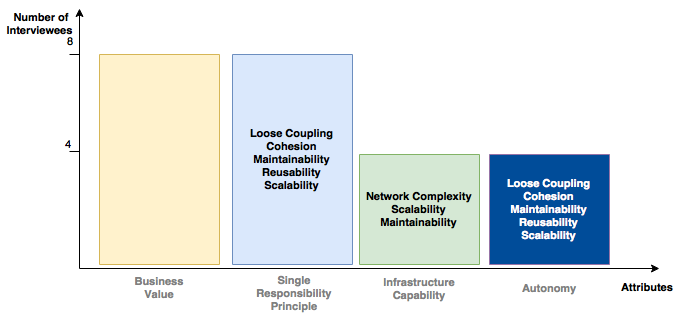
\includegraphics[width=0.8\textwidth]{figures/hybris-architecture-two}
\caption{Attributes grouping from interview response}
\label{fig:hybris_architecture/interview/attributes_grouping}
\end{center}
\end{figure}
\\
The interview unfolded various quality attributes which determine the correct size of a microservice. Moreover, these quality attributes can be classified into three major groups which are: \\
\begin{enumerate}
\item Single Responsibility Principle
\item Automony
\item Infrastructure Capability
\end{enumerate}
\\
Additionally, the response from the question \ref{question:hybris_architecture/interview/question_1.4} highly suggest the significance of availability of proper infrastructure to decide about size of microservices and the microservices architecture.
This highly moves in the direction to support the hypothesis.\\
Finally, there appears one additional constraint to affect the size of microservices, not covered by hypothesis but mentioned by all interviewees, which is the business value provided by the microservices.
\\
\begin{shaded} Hypothesis 2 \end{shaded}
\textbf{Domain driven design is the optimum approach to design microservices.}
\\
From the response to question \ref{question:hybris_architecture/interview/question_3.1}, it can be implied that the organization has no consistent set of specific guidelines which are agreed and pratised across all teams. However,  
the various reactions to the question \ref{question:hybris_architecture/interview/question_3.2} appear to fall with two class of process. The response from \ref{question:hybris_architecture/interview/question_3.2} is repeated here again for convenience \ref{fig:hybris_architecture/interview/process_variations_to_design_microservices}.\\
\\
\begin{figure}[H]
\begin{center}
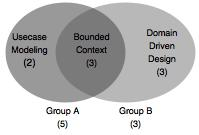
\includegraphics[scale=0.5]{figures/hybris-architecture-three}
\caption{Process variations to design microservices}
\label{fig:hybris_architecture/interview/process_variations_to_design_microservices}
\end{center}
\end{figure}
\\
There is one group of reactions which follow a process to functionally divide a usecase into small functions based upon various factors such as single responsiblity and the requirements of performance. This strongly resemble to the usecase modeling technique as described in the chapter \ref{chapter:selection_by_use_case}. 
\\Moreever, within the same group, a partition are also using the concept of bounded context to ensure autonomy, which also suggests towards the direction of domain driven design as mentioned in the chapter \ref{chapter:domain_driven_design}. It is interesting to find out that some of the teams are using the concept of bounded context implicitly even without its knowledge. The rest of the teams who were not using bounded context, have no idea about the concept. It may be assumed that they will have different view once they get familiar with the concept.
\\
Finally, the rest of the interviewees agree on domain driven design to be the process to design microservices. So, the  response is of mixed nature, both usecase modeling and domain driven design are used in desigining microservices. However, it should also be stated that domain driven design are used on its own or along with usecase modeling to design autonomous microservices.

 \section{Interview Summary}\label{section:hybris_architecture/interview_summary}
Granularity of a microservice is considered as an important aspect when designing microservices architecture. The first impression in major cases is to make the size of microservice as small as possible however there are also various attributes and concepts which affects the decision regarding the size of microservices. The major aspects are single responsibility principle, autonomy and infrastructure capability.
\\
The single responsibility gives impression to assume the size of a microservice as small as possible so that the service has minimum cohesive functionality and less number of consumers affected. Whereas, in order to make the microservice autonomous, the service should have full control over its resources and less dependencies upon other services for accomplishing its core logic. This suggests that the size of the service should be big enough to cover the transactional boundary upon its core logic and have full control on its business resources. 
\\
Moreover, the small the size of the service is, the number of required microservices increases to accomplish the functionalities of the application. This increases network complexity. Additionally, the logical complexity as well as maintainability will increase. Undoubtedly, the independent scalability of individual service will also increase. However, this increases the operational complexity for maintaining and deploying the microservices, due to the number of services and number of environment to be maintained for each services.
\\
The research findings as well as interview response leads to the idea that the question regarding "size" of a microservices has no straight answer. The answer itself is a multiple objective optimization problem whose answer depend upon the level of abstraction of the problem domain achieved, self-governance requirement, self-containment requirement and the honest capability of the organization to handle the operational complexity.
\\
Finally, there is an additional deciding factor called "Business Value". The chosen size of the microservice should give business and competitive advantage to the organization and closely lean towards the organizational goals. A decision for a group of cohesive functionalities to be assigned as a single microservice means that a dedicated resources in terms of development, scaling, maintainance, deployment and cloud resources have to be assigned. A rational decision would be to relate the expected business value of the microservice against the expected cost value required by it.
\\
The teams do not follow any quantitative metrics for measuring various quality attributes such as granularity, coupling and cohesion. According to the reactions from interviews, the basic metrics to evaluate the quality attributes visualized in the table \ref{tab:quality_of_service/quality_attributes/basic_quality_metrics} can be helpful to approach the design of microservices architecture in an efficient way.
\\
There is no single consistent process followed across all the teams. Each team has its own steps to come up with microservices. However, the steps and decision are highly influenced by a set of \abrshort{YaaS} standard principles \ref{section:hybris_architecture/YaaS_architecture_principles}. The reactions from the interviewees are already visualized in \ref{fig:hybris_architecture/interview/process_variations_to_design_microservices}. The process followed by a portion of teams closely relate to usecase modeling approach, where a usecase is divided into several smaller abstractions guided by cohesion, reusability and single responsibility principle. Within this group, a major number of teams also use the concept of bounded concept in order to realize autonomous boundary around the service. Finally, the remaining portion of the teams closely follow domain driven design, where a problem domain is divided into sub-domains and in each sub-domain, various bounded contexts are discovered, which is then mapped into microservices. 
\\
The domain driven design can be considerd as the most suitable approach to design microservices. Following this approach, not only the problem domain is functionally divided into cohesive group of functionalities but also leads to a natural boundary around the cohesive functionalities with respect the real world, where concept as well as differences are well understood and the ownership of business resources and core logic are well preserved.

 \section{Example Scenario}\label{section:hybris_architecture/example_scenario}
 \acrshort{YaaS} provides a cloud platform where customers can buy and sell applications and services. In order to accomplish this, \acrshort{YaaS} offers various basic business and core functionalities as microservices. The customers can either use or extend these services to create new services and applications focusing on their individual requirements and goals.
 \\
The following part of this section discuss the steps used to identify the basic microservices in \acrshort{YaaS}.
\\
\textbf{\underline{Step 1:}}
\\
The problem domain is studied thoroughly to identify core domains, supporting domains and generic domains.
\begin{table}[H]
  \centering
  \begin{adjustbox}{max width=\textwidth}
  \begin{tabular}{*{14}{|c}|}%%{|c|c|c|}
  \hline
  \# & \textbf{Sub-domain}  & \textbf{Type} & \textbf{Description}\\
  \hline
  \hline
   1 & Checkout         & Core          & handles overall process from cart creation to selling of cart items.\\ \hline \hline
   2 & Product          & Supporting    & deals with product inventory\\ \hline
   3 & Customer         & Supporting    & deals with customer inventory\\ \hline
   4 & Coupon           & Supporting    & deals with coupon management \\ \hline
   5 & Order            & Supporting    & handles orders management\\ \hline \hline
   6 & Email            & Generic       & provides REST api for sending emails\\ \hline
   7 & Event            & Generic       & provides asynchronous event based notification service\\ \hline
   8 & Account          & Generic       & handles users and roles management\\ \hline
   9 & OAuth2           & Generic       & provides authentication for clients to access resource of resource-owner \\ \hline 
   \hline
   \end{tabular}
\end{adjustbox}
  \caption{Sub-domains in \acrshort{YaaS}}
  \label{tab:hybris_architecture/example_scenario/sub-domains-in-YaaS}
\end{table}
\\
\textbf{\underline{Step 2:}}
\\
The major functionality of the commerce platform is to sell products, which makes 'Checkout' the core sub-domain. The sub-domain is responsible for a bunch of independent responsibilities. The individual independent functionalities can be rightfully represented by respective bounded contexts. The bounded contexts are realized using microservices. The other major reason for them to be made microservices, in addition to single independent responsibility, is different scalability requirements for each functionality.
\begin{table}[H]
  \centering
  \begin{adjustbox}{max width=\textwidth}
  \begin{tabular}{*{14}{|c}|}%%{|c|c|}
  \hline
  \# & \textbf{Bounded Context}  & \textbf{Description}\\
  \hline
  \hline
   1 & Checkout             & handles the orchestration logic for checkout \\ \hline
   2 & Cart                 & handles cart inventory \\ \hline
   3 & Cart Calculation     & calculates net value of cart considering various constraints such as tax, discount etc. 
   \\ \hline
   \hline
   \end{tabular}
\end{adjustbox}
  \caption{Bounded Contexts in Checkout}
  \label{tab:hybris_architecture/example_scenario/bounded-context-in-Checkout}
\end{table}
\\
\textbf{\underline{Step 3:}}
\\
The supporting sub-domain Product deals with various functionalities related to "Product".
\begin{table}[H]
  \centering
  \begin{adjustbox}{max width=\textwidth}
  \begin{tabular}{*{14}{|c}|}%%{|c|c|}
  \hline
  \# & \textbf{Bounded Context}  & \textbf{Description}\\
  \hline
  \hline
   1 & Category     & manage category of products \\ \hline
   2 & Product      & manage product inventory\\ \hline
   3 & Price        & manage price for products \\ \hline
   \hline
   \end{tabular}
\end{adjustbox}
  \caption{Functional Bounded Contexts in Product}
  \label{tab:hybris_architecture/example_scenario/functional-bounded-contexts-in-Product}
\end{table}
\\
The bounded contexts listed in table \ref{tab:hybris_architecture/example_scenario/functional-bounded-contexts-in-Product} are based upon the independent responsibility and different performance requirement. Additionally, each functionality deals with business entity "Product". However, the conceptual meaning and scope of "Product" is different in each bounded context. "Product" is a polyseme.
\\
Again, there are two more functionalities identified. The first one is a technical functionality to provide indexing of products so that searching of products can be can be efficient. The functionality is generic, technical and independent. It has a different bounded context and can be realized using different microservice. Furthermore, there is a requirement of mashing up information from product, price and category in order to limit the network data from client to each individual service and improve performance. This is realized using a separate mashup service. Also, these functionalities have different performance requirement.
\begin{table}[H]
  \centering
  \begin{adjustbox}{max width=\textwidth}
  \begin{tabular}{*{14}{|c}|}%%{|c|c|}
  \hline
  \# & \textbf{Bounded Context}  & \textbf{Description}\\
  \hline
  \hline
   1 & Algolia Search   & product indexing to improve search performance     \\ \hline
   2 & Product Detail   & provide mashup of product, price and category         \\ \hline
   \hline
   \end{tabular}
\end{adjustbox}
  \caption{Supporting and Generic Bounded Contexts in Product}
  \label{tab:hybris_architecture/example_scenario/supporting-bounded-contexts-in-Product}
\end{table}
\\
The same process is applied for other subdomains to identify bounded contexts within.It is important to notice that the decision to realize the functionalities as microservices not only considered various technical aspects as performance, autonomy etc but also completely different aspect as "business value". The individual microservices such as Product, Category, Checkout have high business value to \acrshort{YaaS} for the reason that they can be sold within a package.
\\
The various microservices designed following the process as mentioned forms a layer of services based on their level of abstraction and reusability. The layers are shown in figure \ref{fig:hybris_architecture/interview/microservices-layers}. The core services are technical generic services used by business services and form the bottom layer. On the top of that are the domain specific business services focused on domain specific business capability. The individual business functionalites provided by business services are then used by Mashup layer to create high level services by orchestrating them.
\\
\begin{figure}[H]
\begin{center}
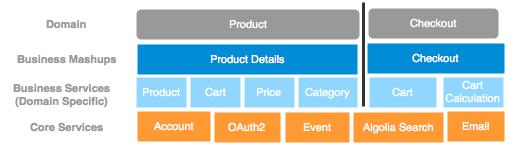
\includegraphics[width=0.8\textwidth]{figures/hybris-architecture-four}
\caption{Microservices Layers}
\label{fig:hybris_architecture/interview/microservices-layers}
\end{center}
\end{figure}
\\
The figure \ref{fig:hybris_architecture/interview/microservices-layers} uncovers only microservices at the backend related to two separate subdomains. The complete architecture covering other domains such as Marketing etc and all layers including User- Interface, \acrshort{PaaS} is shown by figure \ref{fig:hybris_architecture/interview/hybris-architecture}.

\\
\begin{figure}[H]
\begin{center}
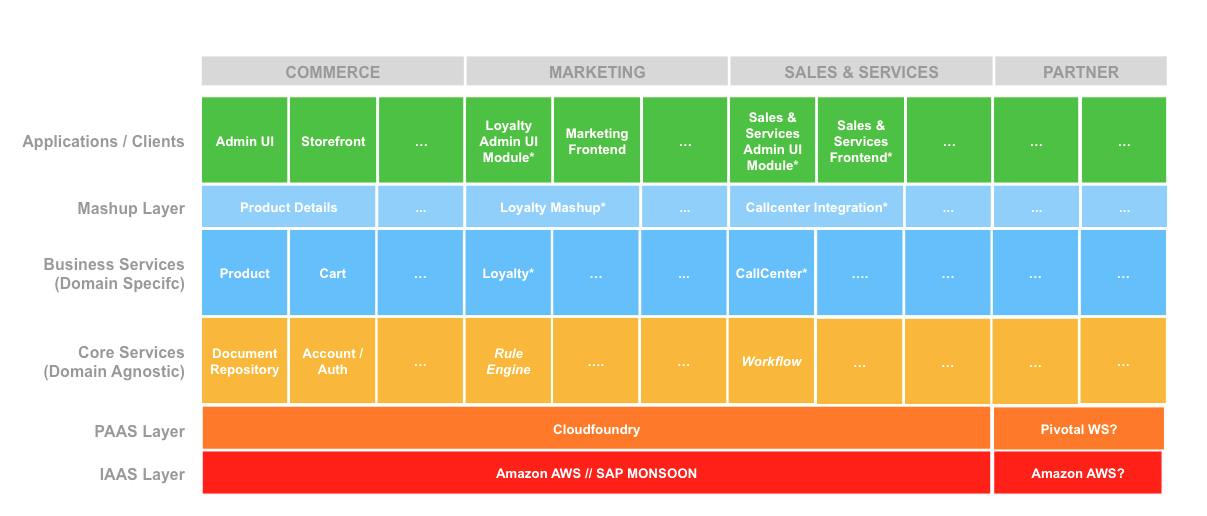
\includegraphics[width=0.9\textwidth]{figures/hybris-architecture-five}
\caption{Hybris Architecture}
\label{fig:hybris_architecture/interview/hybris-architecture}
\end{center}
\end{figure}
\\















%later \chapter{Introduction}\label{chapter:introduction}
Architecture is the set of principles assisting software architect and developers for system or application design. \cite{Dashofy:2009aa} It defines process to decompose a system into modules, components and specifies their interactions. \cite{Brown:2015aa} In this chapter, two different architectural approaches will be taken. Firstly, a conceptual understanding of monolithic architecture style will be presented, which will then be followed by its various advantages and disadvantages. Then, an overview of microservices architecture will be explained. In Section \ref{section:context/motivation}, the motivation for the current research is explained which is then followed by  list of various reseach questions \ref{list:introduction/research_questions} being focused. Finally, in Section \ref{section:context/approach} and Section \ref{section:context/research_strategy}, the approach which will be used to conduct current research is presented. The purpose of this chapter is to provide a basic background context for the following chapters.

\section{Monolith Architecture Style}\label{section:context/monolith}
A Mononlith Architecture Style is one in which an application is deployed as a single artifact. The architecture inside the application can be modular and clean. In order to clarify, the figure \ref{fig:context/monolith-example} shows architecture of an Online-Store application. The application has clear separation of components such as Catalog, Order and Service as well as respective models such as Product, Order etc. Despite of that, all the units of the application are deployed in tomcat as a single war file.\cite{Richardson:2014aa}\cite{Richardson:2014ab}

\begin{figure}[H]
\begin{center}
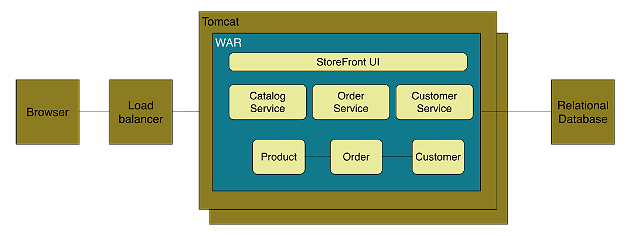
\includegraphics[width=0.7\textwidth]{figures/context-monolith-example}
\caption{Monolith Example from \cite{Richardson:2014aa}}
\label{fig:context/monolith-example}
\end{center}
\end{figure}

\subsection{Types of Monolith Architecture Style}\label{subsection:context/monolith-types}
According to \cite{Annett:2014aa}, a monolith can be of several types depending upon the viewpoint, as shown below:
\begin{enumerate}
\item Module Monolith: If all the code to realize an application share the same codebase and need to be compiled together to create a single artifact for the whole application then the architecture is Module Monolith Architecture. An example is show in Figure \ref {fig:context/module-monolith-example}. The application on the left of the figure, has all the code in the same codebase in the form of packages and classes without clear definition of modules and get compiled to a single artifact. However, the application on the right is developed as a number of modular codebase, each has separate codebase and can be compiled to different artifact. The modules uses the produced artifacts which is different than the earlier case where the code referenced each other directly.
\begin{figure}[H]
\begin{center}
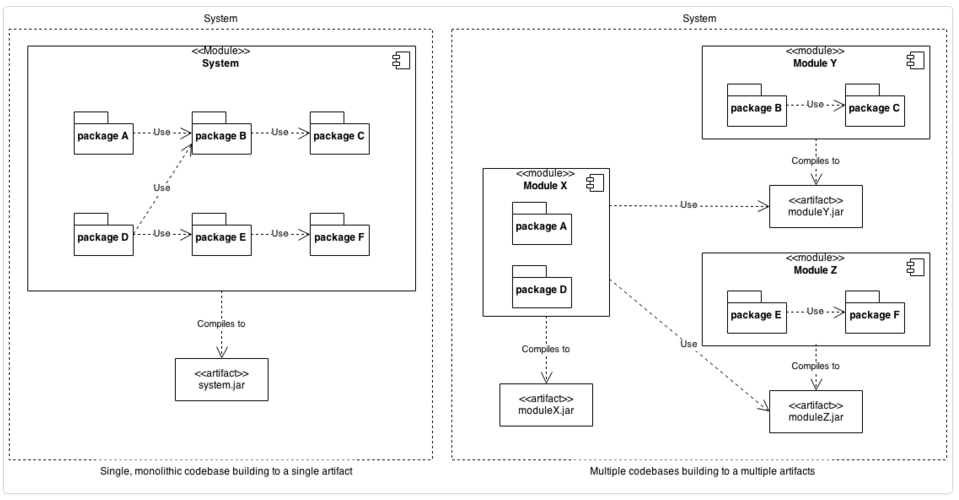
\includegraphics[width=0.8\textwidth]{figures/context-module-monolith}
\caption{Module Monolith Example from \cite{Annett:2014aa}}
\label{fig:context/module-monolith-example}
\end{center}
\end{figure}
\\
\item Allocation Monolith: An Allocation Monolith is created when all code is deployed to all the servers as a single version. This means that all the components running on the servers have the same versions at any time. The Figure \ref{fig:context/allocation-monolith-example} gives an example of allocation monolith. The system on the left have same version of artifact for all the components on all the servers. It does not make any differenct whether or not the system has single codebase and artifact. However, the system on the right as shown in the figure is realized with multiple version of the artifacts in different servers at any time.
\begin{figure}[H]
\begin{center}
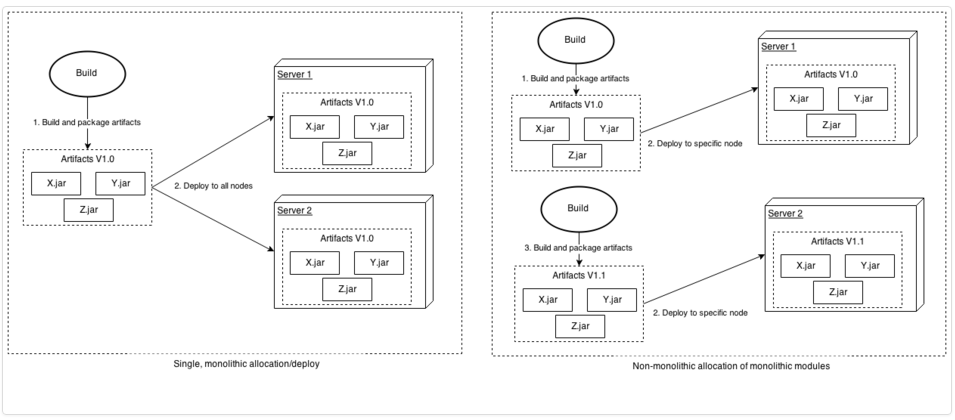
\includegraphics[width=0.8\textwidth]{figures/context-allocation-monolith}
\caption{Allocation Monolith Example from \cite{Annett:2014aa}}
\label{fig:context/allocation-monolith-example}
\end{center}
\end{figure}
\\
\item Runtime Monolith: In Runtime Monolith, the whole application is run under a single process. The left system in the Figure \ref{fig:context/runtime-monolith-example} shows an example of runtime monolith where a single server process is responsible for whole application. Whereas the system on the right has allocated multiple server process to run distinct set of component artifacts of the application.
\begin{figure}[H]
\begin{center}
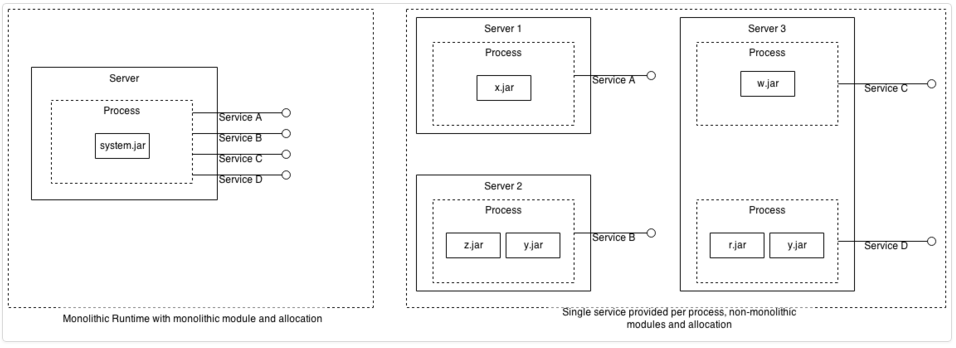
\includegraphics[width=0.8\textwidth]{figures/context-runtime-monolith}
\caption{Runtime Monolith Example from \cite{Annett:2014aa}}
\label{fig:context/runtime-monolith-example}
\end{center}
\end{figure}
\end{enumerate}

\\
\subsection{Advantages of Monolith Architecture Style}\label{subsection:context/monolith-advantages}
The Monolith architecture is appropriate for small application and has following benifits:\cite{Richardson:2014ab}\cite{Fowler:2014aa}\cite{Gupta:2015aa}\cite{Abram:2014aa}
\begin{itemize}[leftmargin=.5in]
\item It is easy to develop a monolith application since various development tools including \acrshort{IDE}s are created around the single application concept. Furthermore, it is also easy to test the application by creating appropriate environment on the developer's machine.
\item The deployment can be simply achieved by moving the single artifact for the application to an appropriate directory in the server.
\item The scaling can be clearly and easily done by replicating the application horizontally across multiple servers behind a load balancer as shown in Figure \ref{fig:context/monolith-example}
\item The different teams are working on the same codebase so sharing the functionality can be easier.
\end{itemize}
\\
\subsection{Disadvantages of Monolith Architecture Style}\label{subsection:context/monolith-disadvantages}
As the requirement grows with time, alongside application becomes huge and the size of team increases, then the monolith architecture faces many problems. The challenges of monolith architecture are as explained below:\cite{Namiot:2014aa}\cite{Newman:2015aa}\cite{Abram:2014aa}\cite{Richardson:2014aa}\cite{Richardson:2014ab}\cite{Gupta:2015aa}
\begin{itemize}[leftmargin=.5in]
\item Limited Agility: As the whole application has single codebase, even changing a small feature to release it in production takes time. Firstly, the small change can also trigger changes to other dependent code. In huge monolith application it is very difficult to manage modularity especially when all the team members are working on the same codebase. Secondly, to deploy a small change in production, the whole application has to be deployed. Thus continuous delivery gets slower. This will be more problematic when multiple changes have to be released on a daily basis. The slow pace and low frequency of release will highly affect agility.
\\
\item Decrease in Productivity: It is difficult to understand the application especially for a new developer because of the size of codebase. Although it also depends upon the structure of the codebase, it will still be difficult to grasp the significance of the code when there is no hard modular boundary. Additionally, a developer can be intimidated due to need to see the whole application at once from outwards to inwards direction. Secondly, the development environment can be slow to load the whole application and at the same time the deployment will also be slow. In overall, it will slow down the speed of understandability, execution and testing.
\\
\item Difficult Team Structure: The division of team as well as assigning tasks to the team can be tricky. Most common ways to partition teams in monolith are by technology and by geography. However, each one cannot be used in all the situations. In any case, the communication among the teams can be difficult and slow. Additionally, it is not easy to assign complete vertical ownership to a team for a particular feature from development to release. If something goes wrong in the deployment, there is always a confusion who should find the problem, either operations team or the last person to commit etc. The approprate team structure and ownership are very important for agility.
\\
\item Longterm Commitment to Technology stack: The technology to use is chosen before the development phase by analysing the requirements and the maturity of current technology at that time. All the teams in the architecture need to follow the same techonology stack throughout the lifecycle of application. However, if the requirement changes then there can be situation when the features can be best solved by different sets of technology. Additionally, not all the features in the application are same so cannot be treated accordingly and cannot be solved by same technology as well. Nevertheless, the technology advances rapidly. So, the solution thought right at the time of planning can be outdated and there can be a better solution available at present. In monolith application, it is very difficult to migrate to new technology stack and it can rather be a painfull process.
\\
\item Limited Scalability: The scaling of monolith application can be performed in either of two ways. The first way is to replicate the application along many servers and dividing the incoming request using a load balancer in front of the servers. Another approach is using identical copies of the application in multiple servers as in previous case but partitioning the database access instead of user request. Both of these scaling approaches improves the capacity and availability of the application. However, the individual requirement regarding scaling for each component can be different but cannot be fulfilled with this approach. Also, the complexity of the monolith application remains the same because we are replicating the whole application. Additionally, if there is a problem in a component the same problem can affect all the servers running the copies of the application, this does not improve resilency.\cite{MacVittie:2014aa}\cite{Namiot:2014aa}
\end{itemize}
\\

\section{Microservice Architecture Style}\label{section:context/microservices_architecture_style}
With monolith, it is easy to start development. But as the system gets bigger and complicated along time, it becomes very difficult to be agile and productive. The disadvantages listed in Section \ref{subsection:context/monolith-disadvantages} outweighs its advantages as the system gets old. The various qualities such as scalability, agility need to be maintained for the whole lifetime of the application and it becomes complicated by the fact that the system needs to be updated side by side because the requirements always keeps coming. In order to tackle these disadvantages, microservices architecture style is followed.\\
Microservices architecture uses the approach of decomposing an application into smaller autonomous components. The following Section \ref{section:context/microservices_architecture_style/decompostion_of_an_application} provides details of various decomposition techniques.

\subsection{Decomposition of an Application}\label{section:context/microservices_architecture_style/decompostion_of_an_application}
There are various ways to decompose an application. This section discuss two different ways of breaking down an application.

\subsubsection{Scale Cube}\label{section:context/microservices_architecture_style/decompostion_of_an_application/scale_cube}
The Section \ref{subsection:context/monolith-disadvantages} specified various disadvantages related to monolith architecture style. The book \cite{Fisher:2015aa} provides a way to solve most of the discussed problems related to agility, scalability, productivity etc. It provides three dimensions of scalability as shown in figure \ref{fig:context/scale-cube} which can be applied alone or simultaneously depending upon the situation and desired goals.

\begin{figure}[H]
\begin{center}
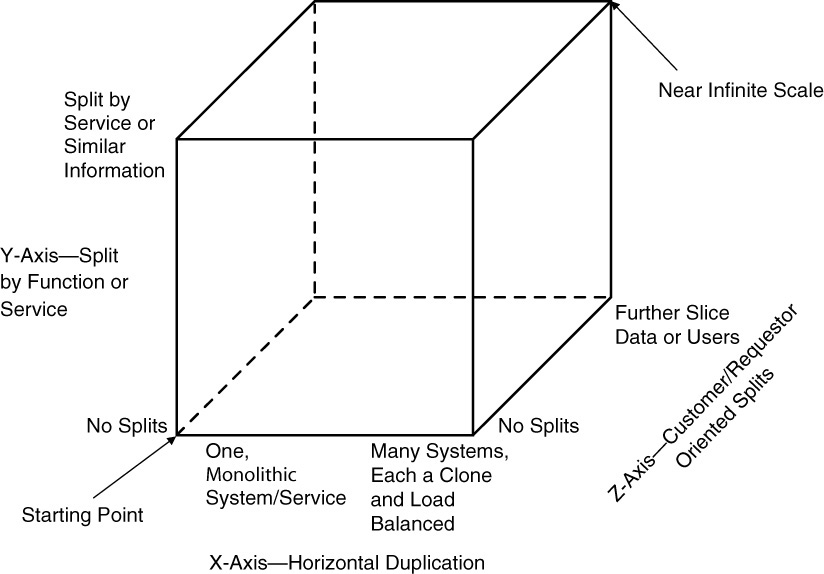
\includegraphics[width=0.5\textwidth]{figures/context-scale-cube}
\caption{Scale Cube from \cite{Fisher:2015aa}}}
\label{fig:context/scale-cube}
\end{center}
\end{figure}

\\
The scaling along each dimensions are described below. \cite{Fisher:2015aa}\cite{MacVittie:2014aa}\cite{Richardson:2014aa}
\begin{enumerate}
\item X-axis Scaling: It is achieved by cloning the application and data along multiple servers. A pool of requests are applied into a load balancer and the requests are deligated to any of the servers. Each of the server has the full capability of the application and full access to all the data required so in this respect it does not make any difference which server fulfills the request. Rather, it is about how many requests are fulfilled at any time. It is easy to scale along X-axis as the number of requests increases. The solution is as simple as to add additional clones. However, with this type of scaling, it does not scale with the increase in data. Moreover, it also does not scale when there are large variation in the frequency of any type of requests or there are dominant requests types because all the requests are handled in an unbiased way and allocated to servers in the same way.
\\
\item Z-axis Scaling: The scaling is obtained by spliting the request based on certain criteria or information regarding the requestor or customer affected by the request. It is different than X-axis scaling in the way that the servers are responsible for different kinds of requests. Normally, the servers have same copy of the application but some can have additional functionalies depending upon the requests expected. The Z-axis scaling helps in fault isolation and transaction scalability. Using this scaling, certain group of customers can be provided added functionality or a new functionality can be tested to a small group and thus minimizing the risk.
\\
\item Y-axis Scaling: The scaling along this dimension means the spliting of the application responsibility. The separation can be done either by data, by the actions performed on the data or by combination of both. The respective ways can be referred to as resoure-oriented or service-oriented splits. While the x-axis or z-axis split were rather duplication of work along servers, y-axis is more about specialization of work along servers. The major advantage of this scaling is that each request is scaled and handled differently according to its necessity. As the logic along with the data to be worked on are separated, developers can focus and work on small section at a time. This will increase productivity as well as agility. Additionally, a fault on a component is isolated and can be handled gracefully without affecting rest of the application. However, scaling along Y-axis can be costly compared to scaling along other dimensions.
\end{enumerate}
\subsubsection{Shared Libraries}\label{section:context/microservices_architecture_style/decompostion_of_an_application/shared_libraries}
Libraries is a standard way of sharing functionalities among various services and teams. The capability is provided by the feature of programming language. However there are various downsides to this approach. Firstly, it does not provide technology heterogeneity. Next, unless the library is dynamically linked, independent scaling, deployment and maintainance cannot be achieved. So, in other cases, any small change in the library leads to redeployment of whole system. Sharing code is a form of coupling which should be avoided.

Decomposing an application in terms of composition of individual features where each feature can be scaled and deployed independently, gives various advantages along agility, performance and team organization as well. Thus, microservices uses the decomposition technique presented by scale cube. A detail advantages of microservices are discussed further in Section \ref{section:challanges_of_microservices_architecture/introduction/challenges}.
\subsection{Definitions}\label{section:context/microservices_architecture_style/definitions}
There are several definitions given by several pioneers and early adapters of the style.
\\
\begin{shaded}Definition 1: \cite{Richardson:2014ac} \end{shaded}
"It is the way to functionally decompose an application into a set of collaborating services, each with a set of narrow, related functions, developed and deployed independently, with its own database."

\\
\begin{shaded}Definition 2: \cite{Wootton:2014aa}\end{shaded}
"It is a style of software architecture that involves delivering systems as a set of very small, granular, independent collaborating services."


\\
\begin{shaded}Definition 3: \cite{Cockcroft:2015aa}\end{shaded}
"Microservice is a loosely coupled Service-Oriented Architecture with bounded contexts."


\\
\begin{shaded}Definition 4: \cite{Fowler:2014aa}\cite{Radchenko:2015aa}\end{shaded}
"Microservices are Service-Oriented Architecture done right."


\\
\begin{shaded}Definition 5: \cite{Fowler:2014aa}\end{shaded}
"Microservice architecture style is an approach to developing a single application as a suite of small services, each running in its own process and communicating with lightweight mechanisms, often an HTTP resource API. These services are built around business capabilities and independently deployable by fully automated deployment machinery. There is a bare minimum of centralized management of these services, which may be written in different programming languages and use different data storage technologies."
\\
As other architectural styles, microservices presents its approach by increasing cohesion and decreasing coupling. Besides that, it breaks down system along business domains following single responsibility principle into granular and autonomous services running on separate processes. Additionally, the architecture focus on the collaboration of these services using light weight mechanisms.

\section{Motivation}\label{section:context/motivation}
The various definitions presented in section highlights different key terms such as:
\begin{enumerate}
\item collaborating services
\item developed and deployed independently
\item build around business capabilities
\item small, granular services
\end{enumerate}
These concepts are very important to be understood in order to approach microservices correctly and effectively. The first two terms relate to runtime operational qualities of microservices whereas the next two address modeling qualities. With that consideration, it indicates that the definitions provided are complete which focus on both aspects of any software applications. \\
However, if attempt is made to have clear indepth understanding of each of the key terms then various questions can be raised without appropriate answers. The various questions (shown in column 'Questions') related to modeling and operations (shown in column 'Type') are listed in the Table \ref{tab:context/microservices_architecture_style/various_questions_related_to_microservices}.
\begin{table}[H]
  \centering
  \begin{adjustbox}{max width=\textwidth}
  \begin{tabular}{*{14}{|c}|}%%{|c|c|}
  \hline
  \# & Questions & Type\\
  \hline
  \hline
   1 & How small should be size of microservices? &  Modeling  \\ \hline
   2 & How does the collaboration among services happen? & Operation  \\ \hline
   3 & How to deploy and maintain independently when there are dependencies among services?& Operation   \\ \hline
   4 & How to map microservices from business capabilities? & Modeling\\ \hline
   5 & What are the challenges need to be tackled and how to? & Operation\\ \hline \hline
   \end{tabular}
\end{adjustbox}
  \caption{Various Questions related to Microservices}
  \label{tab:context/microservices_architecture_style/various_questions_related_to_microservices}
\end{table}
Without clear answer to these questions, it is difficult to say that the definitions presented in Section \ref{section:context/microservices_architecture_style/definitions} are complete and enough to follow the microservices architecture. The process of creating microservices is not clearly documented. There is no enough research papers defining a thorough process of modeling and operating microservices. Additionally, a lot of industries such as amazon, netflix etc are following this architecture but it is not clear about the process they are using to define and implement microservices. The purpose of the research is to have a clear understanding about the process of designing microservices by focusing on following questions.
\begin{shaded}
\textbf{Research Questions}\label{list:introduction/research_questions}
\end{shaded}
\begin{enumerate}
\item How are boundary and size of microservices defined?
\item How business capabilities are mapped to define microservices?
\item What are the best practices to tackle challenges introduced by microservices?
    \begin{enumerate}
    \item How does the collaboration among services happen?
    \item How to deploy and maintain independently when there are dependencies among services?
    \item How to monitor microservices?
    \end{enumerate}
\end{enumerate}
\section{Research Approach}\label{section:context/approach}
A research is an iterative procedure with a goal of collecting as many relevant documents as possible so that the research questions could be answered rationally. So, it becomes very important to follow a consistent research procedure. For the current research, the approach is chosen by refering to \cite{np:2007aa}. It consists of two major phases.
\begin{enumerate}
\item {Data Collection Phase}
\item {Data Synthesis Phase}
\end{enumerate}
The following sections explains each phase in detail.
\subsection{Data Collection Phase}\label{section:context/approach/data_collection_phase}
In this phase, papers related to the reseach questions are collected. The Figure \ref{fig:context/data_collection_phase} shows basic steps in this phase.
\begin{figure}[H]
\begin{center}
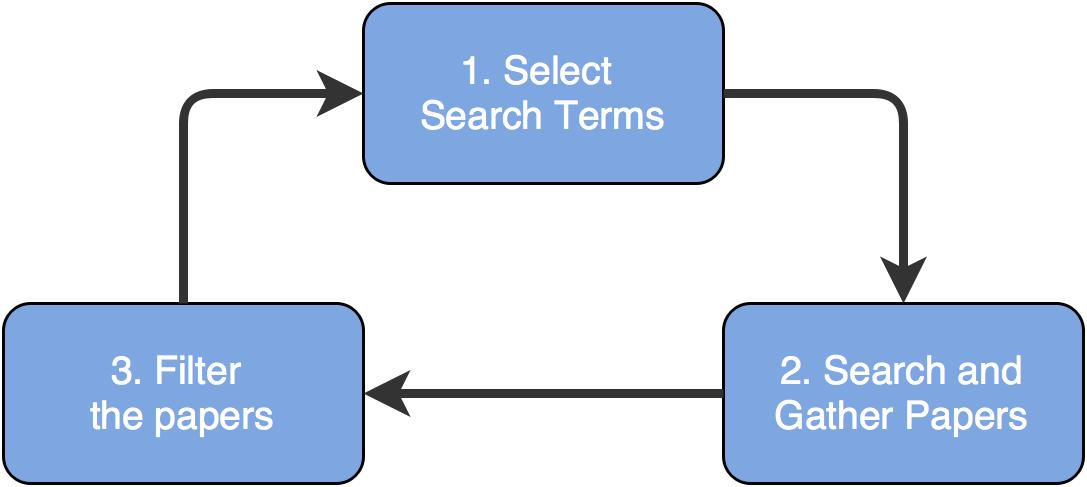
\includegraphics[width=0.8\textwidth]{figures/introduction_data_collection_phase}
\caption{Data Collection Phase}
\label{fig:context/data_collection_phase}
\end{center}
\end{figure}

\begin{enumerate}
\item \textbf{Select Search Terms}\\
At first, various search terms which defines the research topics and questions well, are selected using following strategies.
\begin{enumerate}
\item keywords from research questions and various definitions
\item synonyms of keywords
\item accepted and popular terms from academics and industries
\item references discovered from selected papers
\end{enumerate}
A consise list of initial keywords which are selected from various definitions of microservices are listed in Table \ref{tab:context/microservices_architecture_style/keywords_extracted_from_various_definitions_of_microservice}.
\item \textbf{Search and Gather Papers}\\
The search terms selected in previous step are utilized to discover various papers. In order to achieve that, the search terms are used against various resources listed below.
\begin{enumerate}
\item google scholar
\item IEEExplore
\item ACM Digital Library
\item Researchgate
\item Books
\item Technical Articles
\end{enumerate}
\item \textbf{Filter the Papers}
Finally, the various papers collected from various resources are filtered first to check if the papers have profound base to back up their result. Using only authentic papers is important to provide rational base to current research. The various criteria used to filter the papers are listed below.
\begin{enumerate}
\item Is the paper relevant to answer the research question?
\item Does the paper have good base in terms of sources and provide references of the past studies? 
\item Are there any case studies or examples provided to verify result of the reseach?
\end{enumerate}
\end{enumerate}

\subsection{Data Synthesis Phase}\label{section:context/approach/data_synthesis_phase}
The next phase is to gather data from the selected papers to create meaningful output and provide direction to the research. The Figure \ref{fig:context/data_synthesis_phase} shows various steps within this phase.
\begin{figure}[H]
\begin{center}
\includegraphics[width=0.8\textwidth]{figures/introduction_data_synthesis_phase}
\caption{Data Synthesis Phase}
\label{fig:context/data_synthesis_phase}
\end{center}
\end{figure}

\begin{enumerate}
\item \textbf{Extract Data from selected papers individually}\\
Firstly, each papers are scanned and important data relevant to research are collected.
\item \textbf{Synthesize Data}\\
The data collected from each paper are revised and compared for their similarities in concepts as well as differences in opinion. These individual contents from all papers are then synthesized.
\item \textbf{Create Draft}\\
Finally, draft for the observations are created for future reference which will be used later for creating final report.
\end{enumerate}


\section{Research Strategy}\label{section:context/research_strategy}
The Section \ref{section:context/approach} emphasize the importance of having consistent research procedure. Additionally, it is important to define a good strategy for achieving goals of the research. A good strategy is to narrow down the areas for conducting research. In this section, a list of areas will be identified.\\
The various definitions in Section \ref{section:context/microservices_architecture_style/definitions} show that the authors have their own interpretation of microservices but at the same time agree upon some basic concepts. Nevertheless, each definition can be used to understand different aspect of the microservices. A distinct set of keywords can be identified from these definitions which represents different aspects. The Table \ref{tab:context/microservices_architecture_style/keywords_extracted_from_various_definitions_of_microservice} shows various keywords to focus. Additionally, there are other columns in the table which represents various aspects of microservices architecture. These columns are checked or unchecked to represent the relevancy of each keyword. 

\begin{table}[H]
  \centering
  \begin{adjustbox}{max width=\textwidth}
  \begin{tabular}{*{14}{|c}|}%%{|c|c|c|c|c|c|}
  \hline
  \# & keywords & size & Quality of good microservice & communication & process to model microservices\\
  \hline
  \hline
   1 & Collaborating Services                                       &   &   & \checkmark &  \\ \hline
   2 & Communicating with lightweight mechanism like http           &   &   & \checkmark &  \\ \hline
   3 & Loosely coupled, related functions                           &   & \checkmark  & \checkmark &   \\ \hline
   4 & Developed and deployed independently       &  &   &  & \checkmark \\ \hline
   5 & Own database                                 &  & \checkmark &  & \checkmark \\ \hline
   6 & Different database technologies         &  &  &  & \checkmark \\ \hline
   7 & Service Oriented Architecture  & & \checkmark &  & \checkmark \\ \hline
   8 & Bounded Context  & \checkmark & \checkmark &  & \checkmark \\ \hline
   9 & Build around Business Capabilities  & \checkmark & \checkmark &  &\checkmark \\ \hline
   10 & Different Programming Languages & &  & & \checkmark \\ \hline
   \hline
   \end{tabular}
\end{adjustbox}
  \caption{Keywords extracted from various definitions of Microservice}
  \label{tab:context/microservices_architecture_style/keywords_extracted_from_various_definitions_of_microservice}
\end{table}
Finally, answering various questions around these keywords can be the \textbf{first approach} to understand the topics shown in columns such as size, quality of microservices etc.
\\
The \textbf{next approach} to look around the architecture process is to understand its various drivers. According to \cite{Brown:2015aa}, the important drivers which clarify the architecture are: 
\label{list:introduction/drivers}
\begin{enumerate}
\item \textbf{Quality Attributes}\\
The non-functional requirements have high impact on the resulting architecture. It is important to consider various quality attributes to define the process of architecture.
\item \textbf{Constraints}\\
There are always limitations or disadvantages faced by any architecture however the better knowledge is useful in the process of explaining the architecture with satisfaction.
\item \textbf{Principles}\\
The various principles provides a consistent approaches to tackle various limitations. They are the keys to define guidelines.
\end{enumerate}
So, in order to define the process of modeling microservices, the key aspects related to \textbf{quality attributes}, \textbf{constraints} and \textbf{principles} will be studied thoroughly.
\\
\\
Considering both the Table \ref{tab:context/microservices_architecture_style/keywords_extracted_from_various_definitions_of_microservice} and List \ref{list:introduction/drivers}, the approach to be used to define the guidelines will be to first look deep into various quality attributes influencing microservices architecture. Then, the process of identifying or modeling individual microservices from problem domain will be defined. At first, the research is performed based on various research papers. Then, the approach used by industry adopting microservices architecture will be studied in order to answer the research questions. The study will be performed on SAP Hybris.
Finally, the various constraints or challenges which affects microservices will be identified. 
The results of previous research will be mapped into a form of various principles and these principles will ultimately provide sufficient ground to create guidelines for microservices architecture.

\section{Problem Statement}\label{section:context/problem_statement}
Considering the case that the size of microservice is an important concept and is discussed a lot, but no concrete answer regarding this topic exists. Moreover, the idea of size has a lot of interpretations and no definite answer regarding how small a microservice should be. So, the first step should be to understand the concept of granularity in the context of microservices. Additionally, it would be great if some answers regarding the appropriate size of microservices could be found.

%later \chapter{Literature Review}\label{chapter:literature_review}
\section{Software Architecture}\label{section:software_architecture}


\begin{definition}[Software architecture \cite{bass_sa}]



%later \chapter{System Design}
\label{chapter:system_design}
%later \chapter{Results}
\label{chapter:results}

%later \chapter{Discussions}\label{chapter:discussions}
%later \chapter{Conclusion}\label{chapter:conclusion}
% What you learned
% What went well, bad, surprises, insights
% How you'd do it differently?
The software architecture provides a set of guidelines to decompose a system into subsystems, components and modules. Additionally, it defines the interaction amongst its individual components. Defining an architecture is an important part in software development. So, there should be precise guidelines to implement the architecture.\\
One of the architectural approaches is monolithic architecture in which an application is deployed as a single artifact. With this architecture, a) development, b) deployment and c) scaling is simple as long as the application is small. However, as the application gets bigger and complex, the architecture faces various disadvantages including a) limited agility, b) decrease in productivity, c) longterm commitment to technology stack, d) limited scalability, etc. This is where, a different architectural approach called 'Microservices' comes into play. In this approach, a) an application is composed using different independent, autonomous components, b) each component fulfils a single functionality and  c) each component can be deployed as well as updated independently. However, there are various concepts related to the definitions of microservices such as collaboration, granularity, mapping of business capability, etc. which are not clearly documented. Moreover, there are no proper guidelines how to follow microservices architecture. This is the motivation of the current research. The objective of the research is to clarify various concepts related to the microservices and finally create a precise guidelines for implementing the microservices.\\
In order to achieve that, various definitions provided by different authors are taken as starting point. A list of keywords and areas are selected from them, which are further investigated during the research. Furthermore, various factors such as a) quality attributes, b) constraints and c) principles are considered as the building blocks of any architecture. So, these areas are also considered during the research to create guidelines.\\
Granularity of a microservice is considered as an important concept and is discussed a lot. Granularity is not a one dimensional entity but has three distinct dimensions which are a) functionality, b) data and c) business value. Increase in any of these dimension increases granularity. Also, it is important to consider the concept of 'Appropriate' granularity rather than 'Minimum' sized microservices. Appropriate granularity of any microservice is achieved by three basic concepts: \textbf{Single Responsibility Principle}, \textbf{Autonomy}, and \textbf{Infrastructure capability}.
\\
Adding to that, other quality attributes such as coupling, cohesion, autonomy, etc. are as important as granularity. For that purpose, a list of basic metrics are created to evaluate each quality attributes easily. The quality attributes are not mutually exclusive but related to eachother. The relationship among them is clarified so that it becomes easy to determine the appropriate tradeoffs when necessary.\\
Another important concept which is not clearly documented is the process of identification of microservices and mapping of business capability to microservices. Two different approaches are discussed which are \textbf{Using Use Cases Refactoring} and  \textbf{Using Domain Driven Design}.\\
Use Cases Refactoring utilizes use cases to breakdown a problem domain and refactor them based on various concepts such as similarity in functionality, similarity on entities they act, etc. A discrete set of rules for use cases refactoring are also present. On the other hand, domain driven design uses the concept of ubiquitous language and bounded context to break down a problem domain. A detailed step for each phase is also presented. Furthermore, a case study is broken down into microservices using each approach.\\
Use cases Refactoring is comparatively easier since architects and developers are more familiar with the concept. Domain Driven Design on the other hand, is a complex and iterative procedure. Furthermore, use cases Refactoring considers an entity as a single source of truth for all sub-domains in the entire system. Using this approach does not necessarily produce autonomous microservices but focus more on functionalities. However, the domain driven design using the concept of ubiquitous language and bounded context creates autonomous microservices with single responsibility.\\
After conducting research along various literature, another important part is determining the process followed in industry for which SAP Hybris is chosen. Firstly, various available documents are studied which suggested vision and principles as being the driving force for the process of implementing microservices. In order to understand indepth, interviews are conducted with various key personnels related to \acrshort{YaaS}. A major outcome of the interview is that, in addition to factors such as autonomy, infrastructure capability and Single Responsibility Principle, \textbf{Business Value} of the microservices plays significant role when a) identifying microservices  and b) defining the optimum granularity. Finally, the workflow followed during deployment of microservices in SAP Hybris is also studied in order to clarify the operational approach together with modeling process.\\
Understanding constraints is another important driver of architecture. The approach to handle various constraints can be helpful in defining guidelines. Microservices architecture has various advantages such as strong modularity, agility, independent deployment capability however also presents various challenges for maintaining these advantages. The challenges can be kept into three distinct groups: 
\textbf{Distributed System Complexity}
\textbf{Integration}, and
\textbf{Operational Complexity}.\\
Different challenges along each group are discussed. Additionally, the various techniques which can be used to tackle each  are listed based on the literature. Finally, the techniques used in SAP Hybris to handle each challenge are also mentioned.\\
With all the studies performed, the process of microservices architecture can be disected along two phases:
\textbf{Modeling Phase} and 
\textbf{Operation Phase}.\\
During the modeling phase, problem domain is studied and various internal quality attributes along with business value as well as infrastructure capability are considered. Whereas during operational phase, various challenges are tackled. The effectiveness of modeling phase is visible across various external quality attributes in operation phase. Again, the principles are major driving factor for creating architectural guidelines. The principles along both modeling and operation phase are listed based on the previous findings of the research. Finally, for each principles, a set of guidelines are presented. The guidelines are one of the major outcomes of the research.

%later \chapter{Future Directions}\label{chapter:future_directions}
The current thesis research is conducted on the basis of various academic as well as industrial researches. It would be interesting if the current research could create opportunities for new researches.\\
The Table \ref {tab:quality_of_service/quality_attributes/basic_quality_metrics} listed some basic metrices which can be used to evaluate the quality of microservices. The very first thing which can be done is to find the threshold range that can classify good and bad microservices. A certain number of microservices can be taken as sample from which microservices with high scalability, reusability or other external quality attributes can be filtered out from non performing microservices with low scalability and reusability. Then basic metrices tables can be filled along with their corresponding values for each microservice. These tables can used to find threshold values. The threshold values can be verified further by using them while creating new microservice and checking if their external quality attributes meet the expectations.\\
Another direction of the research can be finding the priority sequence of quality attributes for microservices. From literature, the quality attributes to focus are coupling, cohesion and autonomy. During the interview conducted with SAP Hybris, the quality attributes such as scalability and reusability were given priority when mapping functionalities to microservices. It can be valuable to research further in literature as well as in other industries regarding the priority of quality attributes they choose to identify microservices.\\
Furthermore, the basic metrices table can be leveraged to create a graphical tool which representes various microservices as nodes and connections between them as lines between nodes. It would be benefical if various basic metrices can be evaluated only with \acrshort{API} definitions automatically. Then, the graphical tool can be used to show the various quality attributes using the basic metrices. Depending upon the expected quality, the graphical tool can be used to change the definitiona or \acrshort{API} definition can be changed directly. This can be a great interactive tool for optimizing quality of microservices at design time.\\
Nevertheless, the report can always be used as a base to conduct research on other similar industries as SAP Hybris. It can be interesting to view the result obtained from the study at various different industries.
Given the situation that there are very few literature research done in this area and most of the industries which are using microservices have not openly communicated the whole lifecycle process of microservices, this document can be a very good resource for any company to implement microservices architecture. Additionally, the document can also be a good source for further researches in this area.

%later \chapter{Appendices}\label{chapter:appendices}

\section{CAP Theorem}\label{section:appendices/CAP_theorem}
CAP Theorem was published by scientist Eric Brewer and also called as Brewer's Theorem. There are three major requirements for deploying an application in a distributed environment.
\begin{enumerate}
\item \textbf{Consistency}\\
A functionality of a service is accomplished as a whole or not at all. All the nodes accessing any data see the same version at any given time.
\item \textbf{Availability}\\
The functionalities provided by a service are available and working.
\item \textbf{Partition Tolerance}\\
The partitions which occurs due to problems in the network does not affect the operations of the system unless the whole network fails.
\end{enumerate}
According to the theorem, as the system scales across a number of nodes and the volume of requests increase, it becomes difficult to achieve all the three qualities but to compromise any one of them. \cite{Julian:2009aa}
Network partitions cannot be avoided completely due to the very nature of distributed system and so is the quality of partition tolerance has to be maintained. The choice is the trade off between availability and consistency. It is completely dependent upon business requirement which one to choose. \cite{Peter-Bailis:2013aa}
\section{Eventual Consistency}\label{section:appendices/eventual_consistency}
It is a weaker form of consistency which guarantees all read to a data item return the same value eventually, if no additional updates are performend to the same data item. For any update, only the nodes which are viable and reachable at the moment are updated and the remaining nodes are updated when they are back. \cite{Peter-Bailis:2013aa}
\section{Command Query Responsibility Segregation(CQRS)}\label{section:appendices/CQRS}
In this pattern as shown in the figure \ref{fig:appendices/cqrs}, the conceptual model is divided into two separate models, each one for update and read. It refers to creating different object model handled by different logical processes. The database can be shared, where it acts as integration point but can have different database as well.

\begin{figure}[H]
\begin{center}
\includegraphics[width=0.8\textwidth]{figures/Appendices_one_cqrs}
\caption{CQRS [\cite{Fowler:2011ab}]}
\label{fig:appendices/cqrs}
\end{center}
\end{figure}

\section{Single Responsibility Principle}\label{section:appendices/single_responsibility_principle}
Responsibility is inferred as a reason to change. According to the principle, a service should have a single reson to change. In order to achieve that, a service should perform functionalities which change for the same reason. \cite{Martin:2009aa} \cite{Stine:2014aa}

\appendix{}

\glsaddall{} % add all defined terms to glossary, even if not referenced in text
%\printglossaries{}
\printglossary[type=\acronymtype]

\microtypesetup{protrusion=false}
\listoffigures{}
\listoftables{}
\microtypesetup{protrusion=true}
\printbibliography{}

\end{document}
